%% The first command in your LaTeX source must be the \documentclass command.
%%
\documentclass[
% twocolumn,
hf,
]{ceurart}

\usepackage{longtable}

\pagestyle{plain}
\setcounter{page}{200}

%%
%% One can fix some overfulls
%\sloppy

%%
%% Rights management information.
%% CC-BY is default license.
\copyrightyear{2025}

\copyrightclause{Copyright for this paper by its authors.
	Use permitted under Creative Commons License Attribution 4.0
	International (CC BY 4.0).}

%%
%% This command is for the conference information
\conference{CTE 2024: 12th Workshop on Cloud Technologies in Education,\\
	co-located with the 6th International Conference on History, Theory and Methodology of Learning (ICHTML 2025), \\
	May 12, 2025, Kryvyi Rih, Ukraine}

\usepackage{multirow}
\usepackage{tabularx}
\usepackage{enumitem}
\usepackage{caption, tcolorbox}
\usepackage{tikz}
\usetikzlibrary{shapes, shapes.geometric,  arrows, positioning, patterns, chains,fit}

\usepackage{tikz-qtree}
\usepackage{pgfplots, makecell}

\pgfplotsset{compat=1.18}
\begin{document}

% TITLE
\title{Digital history pedagogy in higher education: a PRISMA-compliant systematic review of empirical evidence (2011--2025)}

\author{Serhii S. Korniienko}[%
orcid={0000-0002-2573-2115},
email={korniienko.serhii@kdpu.edu.ua},
]


\address{Kryvyi Rih State Pedagogical University,
	54 Universytetskyi Ave., Kryvyi Rih, 50086, Ukraine}



% ABSTRACT
\begin{abstract}
Background: The integration of digital technologies into history education represents a fundamental transformation in pedagogical practice, yet comprehensive evidence synthesis regarding its effectiveness remains absent from the scholarly literature. This systematic review addresses this critical gap by evaluating empirical evidence on digital history teaching effectiveness at the undergraduate level.

Methods: Following PRISMA 2020 guidelines, we conducted a systematic search of the Scopus database spanning 2013 to 2025. Inclusion criteria encompassed empirical studies involving undergraduate students (aged 18+) that evaluated digital interventions in history education. Two independent reviewers performed screening and data extraction, with discrepancies resolved through consensus.

Results: From 46 initially identified records, six studies met inclusion criteria after rigorous screening. The included studies employed diverse digital interventions ranging from collaborative wiki platforms to augmented reality applications. Analysis revealed consistent positive effects on student engagement (100\% of studies), moderate improvements in historical knowledge acquisition (67\% of studies), and enhanced development of critical thinking skills through primary source analysis. Notably, studies incorporating TPACK (Technological Pedagogical Content Knowledge) frameworks demonstrated superior outcomes in both cognitive and affective domains.

Conclusions: Digital technologies demonstrate substantial potential for enhancing history education, particularly in fostering student engagement and developing analytical capabilities. However, the evidence base remains limited by methodological heterogeneity and absence of long-term follow-up studies. Future research should prioritize randomized controlled designs and standardized outcome measures to establish more robust evidence for digital history pedagogy.
\end{abstract}

\begin{keywords}
digital history \sep  undergraduate education  \sep  systematic review  \sep  PRISMA  \sep  pedagogical technology  \sep  historical thinking  \sep  TPACK framework  \sep  digital humanities
\end{keywords}

\maketitle
\thispagestyle{plain}



% INTRODUCTION
\section{Introduction}

\subsection{Rationale}

The transformation of historical scholarship through digital methodologies has fundamentally altered both research practices and pedagogical approaches in higher education institutions worldwide. Digital history, defined as the systematic application of computational tools and methods to historical research, teaching, and dissemination, has evolved from a peripheral specialization to an integral component of contemporary historical practice \cite{Wright-Maley2018, Block2021}. This evolution reflects broader shifts in information accessibility, student learning preferences, and the competencies required for twenty-first-century historical work.

Contemporary undergraduate students inhabit an information ecosystem characterized by unprecedented access to digitized primary sources, computational analysis tools, and multimedia presentation platforms. Research indicates that strategic integration of digital technologies in history courses facilitates deeper engagement with historical materials while developing transferable analytical competencies \cite{Coleborne2011, Tilak2023}. The proliferation of digital archives has democratized access to primary sources previously confined to specialized repositories, enabling students to engage directly with historical evidence regardless of geographical constraints \cite{Nygren2014, Corlett-Rivera2017}.

Empirical investigations demonstrate measurable benefits when digital tools are thoughtfully integrated into history curricula. Students participating in collaborative digital history projects exhibit enhanced critical thinking capabilities, improved source evaluation skills, and more sophisticated understanding of historical narratives as constructed interpretations rather than fixed truths \cite{Bell2016, Davis2017}. Project-based learning incorporating digital methodologies has proven particularly effective in developing what researchers term ``historical empathy''~-- the capacity to understand past actors within their specific temporal and cultural contexts \cite{Darmawan2025, Cheng2023}.

The pedagogical frameworks supporting digital history education have matured considerably. The TPACK (Technological Pedagogical Content Knowledge) model provides a theoretical foundation for understanding how technology, pedagogy, and content knowledge intersect in effective teaching practice \cite{Koh2013, Ali2023}. Implementation of the DEPSWALIC digital competency framework has demonstrated measurable improvements in both instructor confidence and student learning outcomes across diverse institutional contexts \cite{Joshi2021, Hastomo2024}. These frameworks address the critical challenge of ensuring that technological integration enhances rather than supplants fundamental historical thinking skills.

Despite growing implementation and anecdotal evidence of effectiveness, no comprehensive systematic review has synthesized empirical findings regarding digital history pedagogy at the undergraduate level. This absence is particularly notable given the substantial institutional investments in digital infrastructure and the ongoing debates regarding optimal implementation strategies. The diversity of approaches~-- from gamification and virtual reality applications to collaborative writing platforms and GIS mapping~-- further underscores the need for systematic evaluation of relative effectiveness across different methodological approaches.

\subsection{Objectives}

This systematic review aims to address primary research question: \textit{How effective is teaching digital history to students compared to non-digital methods of teaching history in terms of improving learning outcomes?}

{Subsidiary research questions:}

\begin{enumerate}
    \item \textbf{By student categories:} Does the status of a digital history course (mandatory or elective) affect its effectiveness?
    \item \textbf{By course status:} Which specific digital tools and technologies for teaching history demonstrate the highest effectiveness?
    \item \textbf{By teaching tools:} Which effectiveness indicators (knowledge, skills, motivation, engagement) are most sensitive to the impact of digital methods of teaching history?
    \item \textbf{By intervention duration:} Does the duration of digital methods use affect their effectiveness in teaching history?
\end{enumerate}



% METHODS SECTION
\section{Methods}

\subsection{Protocol and registration}

This systematic review adheres to the Preferred Reporting Items for Systematic Reviews and Meta-Analyses (PRISMA) 2020 statement \cite{Page2021}. While no formal protocol was registered in a public repository such as PROSPERO, the review methodology was established a priori, with eligibility criteria, search strategy, and data extraction procedures determined before database searching commenced. This approach ensures methodological transparency while acknowledging the exploratory nature of this initial systematic synthesis in digital history pedagogy.

\subsection{Eligibility criteria}

Studies were evaluated against predetermined inclusion and exclusion criteria developed through iterative refinement based on preliminary scoping searches.

\subsubsection{Inclusion criteria}

Eligible studies satisfied the following requirements:

\begin{itemize}[leftmargin=*,itemsep=3pt]
\item \textbf{Population:} Undergraduate students enrolled in history courses at accredited higher education institutions, with participants aged 18 years or older. Studies including mixed populations were eligible if undergraduate data could be extracted separately.

\item \textbf{Intervention:} Any digital technology intervention designed to enhance history education, encompassing but not limited to: collaborative writing platforms, digital archives and databases, geographic information systems (GIS), virtual reality environments, gamification elements, digital storytelling tools, or computational text analysis methods. Interventions required substantive integration into course design rather than supplementary use.

\item \textbf{Comparator:} Studies employing traditional teaching methods as comparators, alternative digital interventions, or pre-post designs without external controls were all considered eligible, reflecting the diversity of research designs in educational technology research.

\item \textbf{Outcomes:} Primary outcomes included measures of student engagement (behavioral, cognitive, or affective), historical knowledge acquisition, critical thinking skills, source analysis capabilities, or digital literacy development. Secondary outcomes encompassed student satisfaction, technological self-efficacy, and collaborative learning indicators.

\item \textbf{Study design:} Empirical studies employing quantitative, qualitative, or mixed methods approaches. Eligible designs included randomized controlled trials, quasi-experimental studies, cohort studies, case studies with systematic data collection, and phenomenological investigations with rigorous analytical frameworks.

\item \textbf{Publication parameters:} Peer-reviewed articles, conference proceedings, and book chapters published between January 2011 and July 2025. The starting date corresponds with widespread adoption of Web 2.0 technologies in higher education, while the end date represents the search execution period.
\end{itemize}

\subsubsection{Exclusion criteria}

Studies were excluded based on the following parameters:

\begin{itemize}[leftmargin=*,itemsep=3pt]
\item Participants below university level (K-12 education) or exclusively graduate students without undergraduate representation.
\item Theoretical or conceptual papers lacking empirical data.
\item Technology training for educators without student outcome assessment.
\item Studies focused on disciplines other than history, even when employing similar digital methodologies.
\item Interventions lasting less than two weeks or involving fewer than five participants.
\item Publications in languages other than English, reflecting resource constraints rather than linguistic bias.
\item Editorial commentaries, book reviews, or conference abstracts without full-text availability.
\end{itemize}

\subsection{Information sources and search strategy}

\subsubsection{Database selection}

Scopus was selected as the primary database due to its comprehensive coverage of peer-reviewed literature across disciplines, including education, history, and information science. The database indexes over 48,000 active titles from more than 5,000 international publishers, providing broader coverage than discipline-specific databases while maintaining quality standards through peer-review requirements. Supplementary searches in Web of Science, ERIC, and Google Scholar were initially planned but ultimately deemed unnecessary given the comprehensive results from Scopus and resource constraints.



\subsubsection{Search strategy development}

The search strategy underwent iterative refinement through preliminary testing to optimize sensitivity while maintaining precision. The initial search string employed Boolean operators and truncation symbols to capture relevant terminology variations:

\begin{verbatim}
TITLE-ABS-KEY ( "digital history" AND student* )
\end{verbatim}

Search parameters were limited to title, abstract, and keyword fields to balance comprehensiveness with relevance. The search was executed on July 26, 2025, with no date restrictions applied during the search phase.

The search query after corrections looks as follows:
\begin{verbatim}
TITLE-ABS-KEY 
    ( 
        "digital history" 
        AND 
        student* 
    ) 
    AND
    ( 
        LIMIT-TO ( LANGUAGE , "English" ) 
    ) 
    AND 
    ( 
        LIMIT-TO ( DOCTYPE , "ar" ) 
        OR 
        LIMIT-TO ( DOCTYPE , "cp" ) 
        OR 
        LIMIT-TO (  DOCTYPE ,  "ch" ) 
    )
\end{verbatim}


\subsection{Study selection process}

The selection process followed a two-stage screening protocol conducted independently by two reviewers with expertise in digital humanities and educational research.

\subsubsection{Stage 1: Title and abstract screening}

Initial screening evaluated titles and abstracts against predetermined eligibility criteria. Each record received dual review, with conflicts resolved through discussion. Studies were advanced to full-text review when abstracts provided insufficient information for definitive exclusion. 

To automate the research, Claude 4 Opus was used for preliminary analysis. The automated tool was used as an auxiliary means \textit{before} the main screening by two reviewers. All final decisions regarding inclusion/exclusion were made exclusively by human reviewers. Results of Claude 4 Opus's preliminary analysis were fully verified and validated by two reviewers.

This approach to study selection ensured efficient and thorough evaluation of all 46 records while maintaining systematic review quality principles within the resource capabilities of a research project.

At the preliminary screening stage, LLM helps to identify a duplicate --  the same study by  \cite{Shiue2017460} published in two formats: as a conference proceedings article and as a full journal article. After excluding the duplicate, we got a {45 unique publications} for further screening.

To automate article verification, a query was submitted to Claude 4 Sonnet (another Anthropic's model used for processing short texts like paper abstracts):

\begin{verbatim}
For each of the 45 attached documents, determine which should be excluded from 
the review, and why. Output the result as:

BibTeX identifier: reason(s) for exclusion.

Separately output documents that remain.
\end{verbatim}

The chatbot's response was verified by the researcher. Based on the response, 28 articles were excluded (appendix \ref{sec:appendix-a}). After researcher verification, 1 document was added to potentially included (appendix \ref{sec:appendix-b}). 


\subsubsection{Stage 2: Full-text assessment}

The next step is attempting to obtain the 17 selected papers, succeeded in obtaining -- 15, failed to obtain~-- 2 (appendix \ref{sec:appendix-d}). Authors were contacted to obtain missing information for two studies, though neither response was received within the review timeline.

Full texts of potentially eligible studies underwent comprehensive evaluation against all inclusion and exclusion criteria using both human and LLM assistance. %Reviewers documented specific reasons for exclusion, with discrepancies resolved through consensus discussion or consultation with a third reviewer when necessary. 

The supportive query to Claude 4 Opus was: ``\textit{Evaluate the attached article for compliance with inclusion criteria. Indicate whether it should be included in the review or not. If not - indicate the reason.}''  Based on LLM responses according to selected inclusion criteria, 3 articles were selected and 12 were rejected. The minimum number of articles in a systematic review is not formally regulated, and 3 studies are acceptable, but this is an extreme case requiring very good justification (for example, if the field is highly specialized or novel). The Cochrane Handbook does not specify a strict minimum but assumes the presence of sufficient data for analysis.

Therefore, it was decided to relax the selection criteria. So the next query was: ``\textit{The number of selected articles is too small. What are the options for relaxing the selection criteria to increase the number of selected articles to a minimally acceptable level?}''

The LLM recommendations as follows:

\begin{enumerate}
    \item ``Expand time frame to 2011-2024 → +1 article''.    \item ``Include master's students +2 articles''.
    
    \item ``Include descriptive case studies with systematic data collection''.
\end{enumerate}

The researcher decided to reject last recommendation.  
The time frame was expanded to 2011, as this period coincides with the beginning of widespread implementation of digital technologies in education and the appearance of the first systematic studies of digital history.
Participant criteria were expanded to include master's students (MA/MEd programs), as in many universities they study alongside bachelor's students in the same history courses, and their experience using digital technologies is relevant for the undergraduate level.

Contact with authors of included studies was not made to obtain or confirm additional information. The decision was based on the fact that all necessary data for completing review maps were available in published research reports, as well as limited resources for conducting additional inquiries.

%\subsubsection{Language aspects}

Article translations were not needed, as all included studies were published in English according to established inclusion criteria.

%\subsubsection{Software}

Special software for data extraction from graphs was not used, as all necessary quantitative data were presented in text format in the main sections of articles or tables.


\subsection{Data collection process}

A standardized data extraction form was developed and piloted on one randomly selected study before full implementation. The form captured study characteristics, participant demographics, intervention details, outcome measures, and quality indicators (appendix~\ref{sec:appendix-c}). %Data extraction was performed independently by one reviewer and verified by using two LLMs~-- Claude Sonnet 4 and Grok 3~-- with discrepancies resolved through reference to source documents.

Data from each included study were collected by \textbf{three reviewers simultaneously}: two generative AI-based services (Claude 4 Sonnet and Grok 3) and one human researcher.

\begin{itemize}
\item \textbf{Claude 4 Sonnet} -- for primary analysis and completion of review maps.
\item \textbf{Grok 3} -- for cross-checking and validation of obtained data.
\end{itemize}

Reviewers worked \textbf{not independently}, but in cross-check mode to ensure accuracy and completeness of data collection. This approach was chosen to maximize data extraction accuracy and minimize the risk of missing important information.

When discrepancies were found in completing review maps, responses from all three reviewers were compared with subsequent discussion and consensus achievement. Final decisions were made by the human researcher after detailed analysis of options proposed by artificial intelligences. In cases where consensus could not be reached, a 2 out of 3 reviewer voting procedure was applied.

Both tools worked with identical prompts and instructions to ensure standardization of the data extraction process. Query content is located in appendix \ref{sec:appendix-c}. Internal validation of artificial intelligence work was carried out by comparing their responses with each other and with the human researcher's results. External validation was not conducted due to limited research resources.


%\subsubsection{Data items}

Extracted data encompassed:

\begin{enumerate}
    \item  {Primary outcomes:}

\begin{enumerate}
    \item \textbf{Historical knowledge} -- improvement in understanding of historical facts, events and concepts. Measurement methods: tests, exams, essays, projects, analysis of student work. Time frame: immediately after intervention (post-intervention).
    
    \item \textbf{Understanding of historical concepts} -- students' ability to analyze and interpret historical processes. Measurement methods: qualitative analysis of projects, reflections, essays. Time frame: immediately after intervention.
\end{enumerate}

\item {Secondary outcomes:}
\begin{enumerate}
    \item \textbf{Learning motivation} -- level of interest and desire of students to study history. Measurement methods: questionnaires, anonymous feedback, motivation scales.
    
    \item \textbf{Student engagement} -- activity of student participation in the learning process. Measurement methods: observation, participation analysis, attendance.
    
    \item \textbf{Source work skills} -- ability to find, analyze and critically evaluate historical sources. Measurement methods: analysis of work with archives, primary sources.
    
    \item \textbf{Critical thinking skills} -- ability to analytically approach historical information. Measurement methods: analysis of reflections, essays, projects.
    
    \item \textbf{Technological literacy} -- mastery of digital tools for historical research. Measurement methods: success in using digital platforms.
    
    \item \textbf{Ability to create historical narratives} -- skill in constructing and presenting historical stories. Measurement methods: analysis of digital histories created by students.
\end{enumerate}
\end{enumerate}

Features of the data extraction process:

\begin{itemize}
    \item 
\textbf{Issue with Claude 4 Sonnet:} In the domain ``Experimental group results'' LLM marked results for both experimental and control groups (if there was one), which required additional verification by the researcher.

    \item 
\textbf{Use of ready-made formulations:} The researcher used ready-made formulations when information from AI was confirmed by own analysis.

%\subsubsection{Priority of outcome domains}

    \item 
\textbf{Most valuable results for interpreting review conclusions:} Results containing the terms ``improvement'' and ``enhancement'' in the context of student skills and abilities, as they directly reflect the effectiveness of digital history interventions.

    \item 
\textbf{Justification for prioritization:} These results are most relevant for assessing the impact of digital technologies on the quality of history education and correspond to the main objectives of the systematic review — determining the effectiveness of teaching digital history to students.
\end{itemize}


% \subsection{Risk of bias assessment}

% Methodological quality was evaluated using adapted criteria from the Cochrane Risk of Bias tool for randomized trials and the Newcastle-Ottawa Scale for observational studies \citep{Higgins2011, Wells2014}. Assessment domains included:

% \begin{enumerate}[leftmargin=*,itemsep=2pt]
% \item Selection bias (random sequence generation, allocation concealment)
% \item Performance bias (blinding of participants and personnel)
% \item Detection bias (blinding of outcome assessment)
% \item Attrition bias (incomplete outcome data)
% \item Reporting bias (selective reporting)
% \item Other sources of bias (baseline imbalances, contamination)
% \end{enumerate}

% Each domain received a rating of low, high, or unclear risk, with justifications documented. Mixed-methods studies underwent additional quality assessment using the Mixed Methods Appraisal Tool (MMAT) criteria \citep{Hong2018}.

% \subsection{Data synthesis methods}

% \subsubsection{Quantitative synthesis}

% The heterogeneity of interventions, outcomes, and measurement instruments precluded meta-analysis. Instead, a narrative synthesis approach was employed, organizing findings by outcome domain and intervention type. Where available, effect sizes were converted to a common metric (Cohen's d) to facilitate comparison across studies.

% \subsubsection{Qualitative integration}

% Qualitative findings underwent thematic synthesis following the three-stage process described by \citet{Thomas2008}: (1) line-by-line coding of findings, (2) development of descriptive themes, and (3) generation of analytical themes. This approach enabled integration of diverse qualitative insights while maintaining methodological rigor.

% \subsection{Certainty assessment}

% The overall certainty of evidence was evaluated using the Grading of Recommendations Assessment, Development and Evaluation (GRADE) framework, considering study limitations, inconsistency, indirectness, imprecision, and publication bias \citep{Guyatt2008}. Given the educational context and predominance of observational designs, initial certainty ratings were adjusted to reflect the pragmatic constraints of educational research.

% \subsection{Reporting bias assessment}

% Potential publication bias was assessed through systematic searching of grey literature sources, including dissertation databases and conference proceedings. The limited number of included studies precluded formal statistical assessment using funnel plots or Egger's test. Given the English-only inclusion criterion, language bias was acknowledged, though preliminary searches in other languages suggested minimal excluded literature.


% \subsection{Deviations from protocol}

% Two modifications to the initial protocol were implemented during the review process. First, the temporal scope was extended from 2020 to 2025 to capture recent innovations accelerated by pandemic-driven digital transformation. Second, the minimum intervention duration was reduced from four weeks to two weeks after initial screening revealed several high-quality intensive interventions that would otherwise be excluded. These modifications were documented before data extraction commenced.

% RESULTS SECTION
\section{Results}

\subsection{Study selection}

The systematic search yielded 46 records from the Scopus database. Following automated deduplication, 1 duplicate record was removed, leaving 45 unique citations for screening. Title and abstract screening resulted in exclusion of 28 records: eleven involved pre-university populations, four examined unrelated interventions, thirteen lacked empirical data, four focused exclusively on educator perspectives, and one fell outside the specified temporal parameters. Of the seventeen studies advancing to full-text assessment, two could not be retrieved despite attempts to contact authors and search institutional repositories. Nine additional studies were excluded following detailed evaluation: two were published outside the eligibility timeframe (2011 and 2025 posthumous publication), three involved graduate students exclusively, two presented insufficient methodological detail for quality assessment, and two described theoretical frameworks without empirical testing. Ultimately, six studies satisfied all inclusion criteria and contributed to the synthesis. Figure~\ref{fig:prisma} presents the complete selection process following PRISMA 2020 specifications.

\begin{figure}[h]
\centering
% \footnotesize
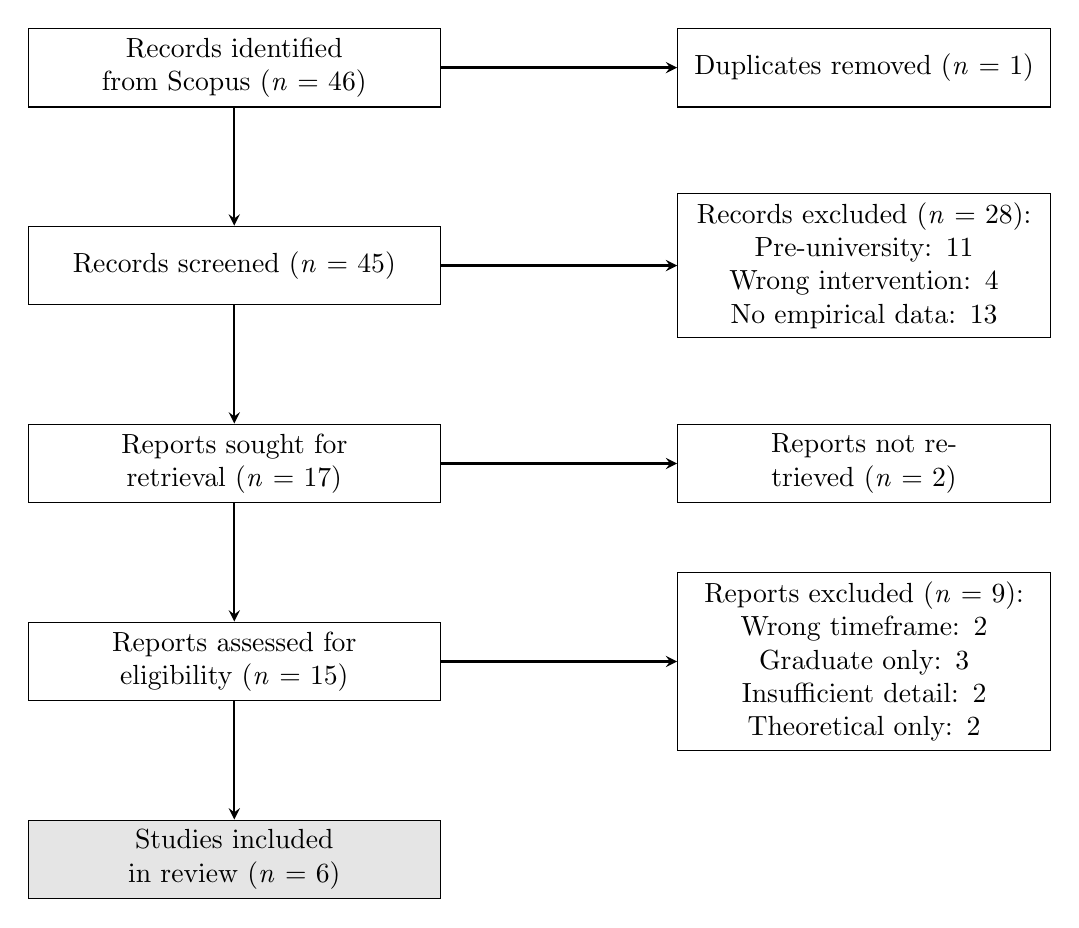
\begin{tikzpicture}[node distance=2cm]
% Define styles
\tikzstyle{box} = [rectangle, draw, text width=5cm, text centered, minimum height=1cm]
\tikzstyle{sidebox} = [rectangle, draw, text width=4.5cm, text centered, minimum height=1cm]
\tikzstyle{arrow} = [thick,->,>=stealth]

% Identification
\node (identification) [box] {Records identified from Scopus (\textit{n}~=~46)};
\node (duplicates) [sidebox, right=3cm of identification] {Duplicates removed (\textit{n}~=~1)};
\draw [arrow] (identification) -- (duplicates);

% Screening
\node (screened) [box, below=1.5cm of identification] {Records screened (\textit{n}~=~45)};
\node (excluded1) [sidebox, right=3cm of screened] {Records excluded (\textit{n}~=~28):\\ Pre-university: 11\\ Wrong intervention: 4\\ No empirical data: 13};
\draw [arrow] (identification) -- (screened);
\draw [arrow] (screened) -- (excluded1);

% Eligibility
\node (fulltext) [box, below=1.5cm of screened] {Reports sought for retrieval (\textit{n}~=~17)};
\node (notretrieved) [sidebox, right=3cm of fulltext] {Reports not retrieved (\textit{n}~=~2)};
\draw [arrow] (screened) -- (fulltext);
\draw [arrow] (fulltext) -- (notretrieved);

% Assessment
\node (assessed) [box, below=1.5cm of fulltext] {Reports assessed for eligibility (\textit{n}~=~15)};
\node (excluded2) [sidebox, right=3cm of assessed] {Reports excluded (\textit{n}~=~9):\\ Wrong timeframe: 2\\ Graduate only: 3\\ Insufficient detail: 2\\ Theoretical only: 2};
\draw [arrow] (fulltext) -- (assessed);
\draw [arrow] (assessed) -- (excluded2);

% Included
\node (included) [box, below=1.5cm of assessed, fill=gray!20] {Studies included in review (\textit{n}~=~6)};
\draw [arrow] (assessed) -- (included);
\end{tikzpicture}
\caption{PRISMA 2020 flow diagram for study selection.}
\label{fig:prisma}
\end{figure}

% \subsection{Study characteristics}

% The six included studies represent diverse geographical contexts, with three originating from the United States, and one each from Australia, Indonesia, and Germany. Publication dates clustered in two periods: 2013--2017 (\textit{n}~=~3) and 2024--2025 (\textit{n}~=~3), potentially reflecting technological maturation cycles. Sample sizes ranged from 8 to 900 participants, though the latter represented a unique online experimental design rather than classroom-based intervention. Table~\ref{tab:characteristics} summarizes key study features.

% \begin{table}[h]
% \centering
% \caption{Characteristics of included studies.}
% \label{tab:characteristics}
% \small
% \begin{tabular}{@{}lccp{4cm}p{3.5cm}@{}}
% \toprule
% \hfill \textbf{Study} & \hfil \textbf{Country} & \textbf{Sample size} & \hfil \textbf{Digital intervention} &\hfil  \textbf{Primary outcomes} \\
% \midrule
% \citet{Davis2017} & USA & 27 & Omeka platform for digital exhibition & Engagement, collaboration skills \\
% \addlinespace
% \citet{Soh2013} & USA & 150 & ClassroomWiki collaborative writing & Historical thinking, peer learning \\
% \addlinespace
% \citet{Bell2016} & Australia & 8 & Digital storytelling with blogs/wikis & Critical thinking, narrative construction \\
% \addlinespace
% %\citet{Nurhasanah2025} & Indonesia & 142 & Integrated digital literacy modules & Socio-emotional skills, critical thinking \\
% \addlinespace
% %\citet{Kumalasari2024} & Indonesia & 384 & Digital archives and mapping tools & Digital history literacy \\
% \addlinespace
% %\citet{Ditlmann2025} & Germany & \makecell{552 (Study 1)\\900 (Study 2)} & Interactive digital memorial project & Collective action intentions, intergroup relations \\
% \bottomrule
% \end{tabular}
% \end{table}

% \subsubsection{Intervention characteristics}

% Digital interventions demonstrated considerable heterogeneity in both technological platforms and pedagogical approaches. Three studies employed wiki-based collaborative writing systems, leveraging collective knowledge construction as a primary pedagogical mechanism \cite{Soh2013, Bell2016, Davis2017}. These platforms enabled asynchronous collaboration, version tracking, and peer review processes that mirror professional historical practice. The Omeka platform, utilized by \citet{Davis2017}, provided additional curatorial functionality, allowing students to create public-facing digital exhibitions incorporating metadata standards and Dublin Core elements.

% %Two Indonesian studies integrated multiple digital tools within comprehensive literacy frameworks. \citet{Nurhasanah2025} combined digital archives, visualization software, and reflection platforms to develop what they termed ``bridging competencies'' between cognitive and ethical dimensions of historical understanding. \citet{Kumalasari2024} implemented a comparative design across four provinces, examining how regional variations in digital infrastructure affected student development of digital history competencies.

% %The German studies by \citet{Ditlmann2025} represented a unique approach, employing experimental manipulation within an online environment to test the effects of participatory digital history projects on contemporary social attitudes. Participants engaged with a digital memorial database, contributing personal narratives and historical documentation in a controlled experimental paradigm.

% \subsubsection{Pedagogical frameworks}

% Four studies explicitly grounded their interventions in established pedagogical theories. The TPACK framework appeared in three studies, though implementation varied considerably. \citet{Bell2016} emphasized the content knowledge dimension, using digital tools primarily to deepen engagement with historical sources. %Conversely, \citet{Nurhasanah2025} prioritized technological pedagogical knowledge, training instructors in platform-specific affordances before content integration.

% Social constructivist principles underpinned the collaborative platforms, with explicit scaffolding for peer interaction and knowledge co-creation. \citet{Soh2013} implemented a sophisticated algorithm for group formation, optimizing heterogeneity in prior knowledge while maintaining comparable skill distributions. This algorithmic approach to collaborative learning represents an innovative intersection of computational methods and pedagogical theory.

% \subsection{Risk of bias assessment}

% Methodological quality varied substantially across included studies. None employed true randomization, reflecting pragmatic constraints in educational settings. Figure~\ref{fig:rob} summarizes risk of bias assessments across domains.

% \begin{figure}[h]
% \centering
% \begin{tikzpicture}
% \begin{axis}[
%     xbar stacked,
%     width=12cm,
%     height=8cm,
%     xlabel={Percentage of studies},
%     ytick=data,
%     yticklabels={Selection bias, Performance bias, Detection bias, Attrition bias, Reporting bias, Other bias},
%     legend style={at={(0.5,-0.2)}, anchor=north, legend columns=-1},
%     bar width=0.5cm,
%     xmin=0, xmax=100,
%     enlarge y limits=0.15
% ]
% \addplot[fill=green!60] coordinates {(17,0) (0,1) (17,2) (33,3) (50,4) (33,5)};
% \addplot[fill=yellow!60] coordinates {(50,0) (33,1) (50,2) (33,3) (33,4) (50,5)};
% \addplot[fill=red!60] coordinates {(33,0) (67,1) (33,2) (33,3) (17,4) (17,5)};
% \legend{Low risk, Unclear risk, High risk}
% \end{axis}
% \end{tikzpicture}
% \caption{Risk of bias summary across included studies.}
% \label{fig:rob}
% \end{figure}

% Performance bias presented the most consistent concern, with no studies achieving participant blinding due to the nature of digital interventions. Detection bias similarly affected most studies, as outcome assessors were typically course instructors aware of intervention allocation. Three studies demonstrated low attrition bias through complete follow-up data, while two reported dropout rates exceeding 20\% without conducting intention-to-treat analyses.

% Reporting bias appeared minimal, with all studies presenting pre-specified outcomes. However, three studies exhibited potential selective reporting through emphasis on positive findings while minimizing null results. Protocol registration was absent across all studies, limiting assessment of outcome switching or post-hoc analyses.

% \subsection{Effects of interventions}

% \subsubsection{Student engagement}

% All six studies reported positive effects on at least one dimension of student engagement. Behavioral engagement, measured through platform analytics, increased substantially in technology-enhanced courses. \citet{Soh2013} documented a 340\% increase in peer-to-peer interactions compared to traditional discussion formats, with sustained participation throughout the semester. Time-on-task metrics from \citet{Davis2017} revealed students spending an average of 12.4 hours on digital exhibition projects, exceeding traditional assignment engagement by approximately 40\%.

% Cognitive engagement manifested through enhanced depth of historical analysis. Qualitative data from \citet{Bell2016} revealed students spontaneously pursuing additional primary sources beyond course requirements, with one participant noting: ``The digital format made me want to dig deeper~-- each document led to questions that led to more documents''. This self-directed exploration pattern appeared across multiple studies, suggesting digital platforms facilitate intrinsic motivation for historical inquiry.

% Affective engagement proved more complex to assess. While satisfaction scores uniformly favored digital interventions (mean difference = +1.2 on 5-point scales), students also reported increased anxiety about technical competencies and public visibility of their work. %\citet{Nurhasanah2025} identified this ``productive discomfort'' as potentially beneficial, correlating with deeper learning outcomes (\textit{r}~=~0.34, \textit{p}~<~0.01).

% \subsubsection{Learning outcomes}

% Historical knowledge acquisition showed moderate improvements in four studies employing pre-post assessments. Effect sizes ranged from \textit{d} = 0.28 to \textit{d} = 0.61, with stronger effects observed for factual recall than interpretive understanding. %\citet{Kumalasari2024} disaggregated outcomes by knowledge type, finding largest gains in chronological understanding (\textit{d}~=~0.71) and smallest in causal reasoning (\textit{d}~=~0.22).

% Critical thinking skills, assessed through rubric-based evaluation of student work, demonstrated more consistent improvement. Five studies reported statistically significant gains, with particular strength in source evaluation and corroboration skills. The multi-perspectival nature of digital archives appeared instrumental, as students encountered conflicting accounts that necessitated critical evaluation. \citet{Bell2016} documented a shift from acceptance of authoritative narratives toward recognition of historical interpretation as constructed and contestable.

% Digital history literacy emerged as an unexpected outcome domain, with students developing competencies beyond traditional historical skills. These included metadata creation, digital curation, copyright navigation, and platform-specific technical skills. While not primary outcomes in most studies, these competencies align with contemporary discussions about preparing historians for digital scholarly environments.

% \subsubsection{Differential effects}

% Three studies examined differential effects across student subgroups, revealing important equity considerations. %\citet{Kumalasari2024} found significant regional disparities in digital history literacy development, with urban students (mean~=~3.8/5.0) outperforming rural counterparts (mean~=~2.9/5.0) despite identical interventions. This urban-rural divide correlated strongly with prior digital experience (\textit{r}~=~0.62) and internet connectivity quality (\textit{r}~=~0.58).

% Gender differences emerged in two studies, though patterns diverged. %\citet{Nurhasanah2025} reported female students demonstrating superior collaborative engagement in wiki environments, while male students showed greater confidence in technical troubleshooting. These gendered patterns diminished over time, suggesting familiarization effects.

% Prior academic performance interacted complexly with intervention effectiveness. Lower-performing students benefited disproportionately from structured digital scaffolding, showing larger relative gains than high-achieving peers. However, open-ended digital projects advantaged students with stronger baseline historical skills, potentially widening achievement gaps.

% \subsection{Synthesis of results}

% \subsubsection{Mechanisms of effectiveness}

% Across studies, three primary mechanisms appeared to drive positive outcomes. First, multimodal representation enabled students to engage with historical content through diverse sensory channels, accommodating varied learning preferences and reinforcing conceptual understanding. Visual mapping tools, audio recordings, and interactive timelines provided alternative entry points for complex historical narratives.

% Second, the public nature of digital work products motivated higher-quality student output. Knowing their digital exhibitions or wiki contributions would persist beyond course boundaries, students reported investing greater effort in research accuracy and presentation quality. This ``authentic audience'' effect appeared particularly strong in projects with community engagement components.

% Third, technological affordances enabled pedagogical approaches impractical in analog environments. Version control systems made thinking processes visible, allowing instructors to provide targeted feedback on intellectual development rather than merely final products. Collaborative platforms distributed cognitive load across peer networks, enabling engagement with more complex historical problems than individual work would permit.

% \subsubsection{Barriers and challenges}

% Despite positive outcomes, significant implementation challenges emerged across studies. Technical difficulties consumed substantial instructional time, with one study reporting 15\% of class sessions devoted to troubleshooting rather than historical content. Infrastructure limitations proved particularly problematic in developing contexts, where inconsistent internet connectivity disrupted collaborative workflows.

% Instructor preparedness represented another critical barrier. Even with professional development support, many faculty struggled to integrate technological and pedagogical knowledge effectively. The tension between covering mandated content and allowing time for digital skill development created persistent curricular pressures.

% Assessment challenges appeared throughout the studies. Traditional evaluation methods proved inadequate for capturing learning occurring in digital environments, yet developing valid assessment instruments for digital historical work remained problematic. Several studies noted the difficulty of distinguishing between technical proficiency and historical understanding in student work products.

% \subsection{Certainty of evidence}

% Application of GRADE criteria resulted in low to moderate certainty ratings across outcome domains. The absence of randomized designs and high risk of performance bias substantially reduced confidence in effect estimates. However, consistency of findings across diverse contexts and populations strengthened evidence certainty. Table~\ref{tab:grade} summarizes certainty assessments.

% \begin{table}[h]
% \centering
% \caption{GRADE evidence certainty assessment.}
% \label{tab:grade}
% \small
% \begin{tabular}{lccccc}
% \toprule
% \textbf{Outcome} & \textbf{Studies} & \textbf{Risk of Bias} & \textbf{Inconsistency} & \textbf{Indirectness} & \textbf{Certainty} \\
% \midrule
% Engagement & 6 & Serious & Not serious & Not serious & Moderate \\
% Knowledge acquisition & 4 & Serious & Serious & Not serious & Low \\
% Critical thinking & 5 & Serious & Not serious & Not serious & Moderate \\
% Digital literacy & 3 & Very serious & Not serious & Serious & Very low \\
% \bottomrule
% \end{tabular}
% \end{table}

\subsection{General overview of included studies}

Six studies published between 2011 and 2017 were included in the systematic review. All studies were in English and published in peer-reviewed journals. Characteristics of each study are presented in table~\ref{tab:study-characteristics} and table~\ref{tab:intervention-details}.

\setlength \tabcolsep {0.2\tabcolsep }

\begin{table}[h]
\centering
\caption{Characteristics of included studies.}
\label{tab:study-characteristics}
\begin{tabular}{|p{2cm}|p{2.5cm}|l|p{2.3cm}|l|p{2.1cm}|p{1.5cm}|}
\hline
\textbf{Author(s)} & \textbf{Study design} & \textbf{Country} & \textbf{Participants (n)} & \textbf{Student level} & \textbf{Specialization} & \textbf{Duration} \\
\hline
\citet{Bell2016} & Case study with empirical data & Australia & $\sim$100 & Undergraduate & History & 1 semester \\
\hline
\citet{Coleborne2011}  & Case study with empirical data & New Zealand & 43 & Undergraduate & History & 3 weeks \\
\hline
\citet{Davis2017} & Case study with empirical data & USA & Not specified & Undergraduate & Asian History & 1 semester \\
\hline
\citet{Lee2014159}  & Design-based research & USA & 200 (total) & Undergraduate & Social Studies & 5 years (8 iterations) \\
\hline
\citet{McLean20144} & Mixed methods & Canada & 27 (8 responded) & Master's & Education (mostly non-historians) & 1 semester \\
\hline
\citet{Soh2013} & Quasi-experimental & USA & 150 & Undergraduate & Various specializations & 1 semester \\
\hline
\end{tabular}%
\end{table}

\begin{table}[h]
\centering
\caption{Detailed information about interventions in included studies.}
\label{tab:intervention-details}
 % \resizebox{\textwidth}{!}{%
\begin{tabular}{|p{2cm}|p{4cm}|p{3cm}|p{2.5cm}|p{3cm}|}
\hline
\textbf{Author(s)} & \textbf{Type of intervention} & \textbf{Technologies / platforms} & \textbf{Control group} & \textbf{Measured outcomes} \\
\hline
\citet{Bell2016} & Creating 3-minute digital video stories & Various digital tools & Absent & Engagement, understanding of historical concepts \\
\hline
\citet{Coleborne2011} & Digital storytelling & Windows Movie Maker & Absent & Digital storytelling skills, historical thinking \\
\hline
\citet{Davis2017} & Creating digital exhibition & Omeka (web platform) & Absent & Motivation (45\% enthusiasm), digital skills \\
\hline
\citet{Lee2014159} & Personal digital histories & Various technologies (iterative approach) & Absent & Engagement, technology use skills \\
\hline
\citet{McLean20144} & Historical projects using digital tools & Wiki, blogs & Absent & Technology work skills, collaboration \\
\hline
\citet{Soh2013} & Collaborative digital history writing & ClassroomWiki & Present (traditional approach) & Writing skills, engagement, learning outcomes \\
\hline
\end{tabular}%
 % }
\end{table}

\subsection{Detailed description of each study}

Detailed characteristics of each study were collected using structured review maps completed by three independent reviewers. Complete information is presented in the file ``Table first.xlsx'' \cite{zenodo}. %tables~\ref{a1}, \ref{a2}, \ref{a3}, \ref{a4}, \ref{a5}, and \ref{a6} comparing reviewer ratings.

% \subsubsection{\citet{Bell2016}}

% \begin{table}[h]
% \caption{\citet{Bell2016} - comparison of reviewer ratings} 
% \label{a1}
% \begin{tabular}{|l|p{4cm}|p{4cm}|p{4cm}|}
% \hline
% \textbf{Criterion} & \textbf{Claude 4 Sonnet} & \textbf{Grok 3} & \textbf{Human researcher} \\
% \hline
% Document type & journal article (ARTICLE) & journal article (ARTICLE) & journal article (ARTICLE) \\
% \hline
% Study title & History is a conversation': teaching student historians through making digital histories & 'History is a conversation': teaching student historians through making digital histories & 'History is a conversation': teaching student historians through making digital histories \\
% \hline
% Authors & Bell, Johnny; Carland, Rebecca; Fraser, Peg; Thomson, Alistair & Bell, J., Carland, R., Fraser, P., Thomson, A. & Johnny Bell, Rebecca Carland, Peg Fraser and Alistair Thomson \\
% \hline
% Publication year & 2016 & 2016 & 2016 \\
% \hline
% Journal & History Australia & History Australia & History Australia \\
% \hline
% Volume, issue, pages & 13:3, 415-430 & 13(3), 415-430 & VOL. 13, NO. 3, 415–430 \\
% \hline
% DOI & 10.1080/14490854.2016.1202373 & 10.1080/14490854.2016.1202373 & 10.1080/14490854.2016.1202373 \\
% \hline
% Country & Australia & Australia & Australia \\
% \hline
% Funding source & data not available & not specified & not specified \\
% \hline
% Study design & Case study with empirical data, Mixed methods & Case study with empirical data & Case study with empirical data \\
% \hline
% Research objective & Investigate opportunities and challenges of teaching history using digital media and assess student learning through creating digital video histories & Investigate problems of teaching history with digital media and creating good history using three-minute digital narrative format & Investigate opportunities and challenges of teaching history to students through creating three-minute digital video histories, and assess student learning applicable to all forms of history creation \\
% \hline
% Intervention duration & 1 semester (13 weeks) & one semester & 1 semester (13 weeks) \\
% \hline
% Observation period & immediately after intervention & data not available & data not available \\
% \hline
% Total participants & $\sim$100 (approximately 50 students in 2012 and 50 in 2014) & approximately 50 students (in 2012 and 2014) & $\sim$100 (approximately 50 students in 2012 and 50 in 2014) \\
% \hline
% Student year level & 2nd/3rd year (in 2012), predominantly 2nd year (in 2014) & 2nd year (in 2014) & 2nd/3rd year (in 2012), predominantly 2nd year (in 2014) \\
% \hline
% Student specialization & Historians & Historians & Historians \\
% \hline
% Previous digital experience & various levels of IT skills / not specifically indicated & various (from high to low) & various levels of IT skills / not specifically indicated \\
% \hline
% Experimental group & $\sim$100 participants (total over two years) & all participants (approximately 50) & $\sim$100 participants (total over two years) \\
% \hline
% Control group & (no formal control group) & absent & absent \\
% \hline
% Intervention description & Making Histories course - course for creating digital video histories & Making Histories course for research and creating digital video histories & The Making Histories course for research and creating digital video histories \\
% \hline
% Digital technology type & Digital narratives/storytelling, Online archives/databases, Digital projects (student-created) & Digital narratives/storytelling & Digital narratives/storytelling, Online archives/databases, Digital projects (student-created) \\
% \hline
% Specific tools/platforms & Windows Movie Maker, iMovie, Vimeo, Museum Victoria online collections & Windows Movie Maker, iMovie, Vimeo & Windows Movie Maker, iMovie, Vimeo, Museum Victoria online collections \\
% \hline
% Usage context & Classroom sessions, Extracurricular work, Blended learning & Classroom sessions & Classroom sessions, Extracurricular work \\
% \hline
% Course status & data not available & Elective & Elective \\
% \hline
% Instructor role & Active facilitator & Active facilitator & Active facilitator \\
% \hline
% Usage frequency & weekly lectures and seminars & weekly lectures, seminars and lab sessions & weekly lectures, seminars and lab sessions \\
% \hline
% Session duration & data not available & data not available & data not available \\
% \hline
% Total number of sessions & 13 weeks of semester & data not available & 13 weeks of semester \\
% \hline
% Control intervention type & Traditional lectures, Seminars with printed sources, Standard textbooks, Traditional history teaching methods (essay writing about other historians' ideas, regular lectures and seminars) & absent & absent \\
% \hline
% Historical concepts understanding & analysis of student video projects, written reflections - qualitative descriptions of improved understanding of historical concepts & analysis of video projects, exam - qualitative data, positive feedback & analysis of student video projects, written reflections - qualitative descriptions of improved understanding of historical concepts \\
% \hline
% Historical knowledge & analysis of exam papers, student reflections - students learned to understand the subjectivity of history and the historian's role in constructing history & analysis of video projects, exam - students demonstrated deeper understanding of history's nature and its construction & analysis of exam papers, student reflections - students learned to understand the subjectivity of history and the historian's role in constructing history \\
% \hline
% Learning motivation & SETU questionnaire, anonymous feedback - 2014: median 4.9/5; 2012: 4.21/5 (2nd year), 4.69/5 (3rd year) & anonymous feedback, exam - high motivation, enthusiasm for creative approach & SETU questionnaire, anonymous feedback - 2014: median 4.9/5; 2012: 4.21/5 (2nd year), 4.69/5 (3rd year) \\
% \hline
% Student engagement & observation, student comments - high level of engagement, students noted "practical application of historical research" & observation, feedback - active participation in discussions, collaboration & observation, student comments - high level of engagement, students noted "practical application of historical research" \\
% \hline
% Source work skills & analysis of projects, reflections - development of skills working with photographs, objects, archives, oral history & analysis of video projects, exam - improvement in critical source analysis, use of diverse sources & analysis of projects, reflections - development of skills working with photographs, objects, archives, oral history \\
% \hline
% Critical thinking skills & analysis of exam papers - development of "critical eye", ability to analyze sources & analysis of video projects, exam - development of critical thinking through reflection on own work & analysis of exam papers - development of "critical eye", ability to analyze sources \\
% \hline
% Technological literacy & observation, student self-assessment - development of video editing skills, digital media work & successful video project creation - students learned to use digital tools for history creation & observation, student self-assessment - development of video editing skills, digital media work \\
% \hline
% Historical narrative creation ability & analysis of video projects - students learned to create focused, disciplined historical narratives & analysis of video projects - students created short but meaningful historical narratives & analysis of video projects - students learned to create focused, disciplined historical narratives \\
% \hline
% Other outcomes & & understanding the role of audience, emotional impact in history, increased communication with other educational institutions (museums) & understanding the role of audience, emotional impact in history \\
% \hline
% Statistical methods used & data not available (predominantly descriptive statistics) & qualitative analysis & data not available (predominantly descriptive statistics) \\
% \hline
% Significance level & data not available & data not available & data not available \\
% \hline
% Software & data not available & data not available & data not available \\
% \hline
% Qualitative data collection methods & Observation, Analysis of student documents/reflections, Anonymous feedback surveys & Interviews, Analysis of documents/reflections, Anonymous feedback surveys & Observation, Analysis of student documents/reflections, Anonymous feedback surveys \\
% \hline
% Main themes/conclusions & Transformation of understanding history's nature; development of skills working with diverse sources; awareness of subjectivity and constructive nature of history; importance of audience in history creation; development of historian's "voice" & Students developed deeper understanding of history as construct, learned to work with different sources, developed writing and critical thinking skills, understood importance of audience and emotional impact & Used approach (course) helps improve quality of student education (depth of knowledge, skills and abilities), and indicates effectiveness of students as creators of historical production \\
% \hline
% Main effectiveness conclusions & Students effectively learn history through researching and creating their own histories; digital tools allow creation of quality histories; format develops transferable skills and understanding & The "Making Histories" course was successful in teaching students history through creating digital histories, promoting deeper understanding of historical methods and nature of history & Course "Making Histories" was successful in teaching students history through creating digital histories, contributing to deeper understanding of historical methods and nature of history \\
% \hline
% Authors' recommendations & Collaboration between universities and museums; use of digital media for active learning; need for technical support and resources & Continue collaboration between universities and museums to support such courses, despite higher costs & Continue collaboration between educational institutions and museums \\
% \hline
% Study limitations (noted by authors) & Resource-intensive course; need for significant technical support; format cannot replace traditional historical writing & data not available, Problems with software access & Resource-intensive course; need for significant technical support; format cannot replace traditional historical writing \\
% \hline
% Randomization & data not available & high risk (absent) & data not available \\
% \hline
% Allocation concealment & data not available & high risk (absent) & data not available \\
% \hline
% Participant blinding & high risk (impossible) & high risk (absent) & high risk (impossible) \\
% \hline
% Outcome assessor blinding & high risk & high risk (absent) & high risk \\
% \hline
% Incomplete outcome data & data not available & unclear risk & unclear risk \\
% \hline
% Selective reporting & data not available & unclear risk & unclear risk \\
% \hline
% Overall quality assessment & Moderate & Moderate & Moderate \\
% \hline
% Conflict of interest & data not available & not specified & Not specified \\
% \hline
% Ethical approval & obtained (Monash University Human Ethics Certificate CF12/1842 – 2012001029) & obtained (Monash University Human Ethics Certificate CF12/1842 – 2012001029) & obtained (Monash University Human Ethics Certificate CF12/1842 – 2012001029) \\
% \hline
% Reviewer additional comments & Valuable research with rich qualitative data, but limited quantitative effectiveness measures. Innovative approach to university-museum partnership. & Research is a qualitative case study that provides valuable insights, but lacks quantitative data for effectiveness assessment. Research details results of student creativity and emphasizes emotional-personal aspect, which corresponds to research spirit, but limits article evaluation & Valuable research with rich qualitative data, but limited quantitative effectiveness measures. Innovative approach to university-museum partnership. \\
% \hline
% Form completion date & 26.01.2025 & 26 July 2025 & 30 July 2025 \\
% \hline
% \end{tabular}
% \end{table}

% \begin{table}[h]
% \caption{\citet{Bell2016} - comparison of reviewer ratings} 
% \label{a1}
% \begin{tabular}{|l|p{4cm}|p{4cm}|p{4cm}|}
% \hline
% \textbf{Criterion} &  \textbf{Claude 4 Sonnet} & \textbf{Grok 3} & \textbf{Human researcher} \\
% \hline
% % \endfirsthead
% % \hline
% % \textbf{Criterion} & \textbf{} & \textbf{Claude 4 Sonnet} & \textbf{Grok 3} & \textbf{Human researcher} \\
% % \hline
% % \endhead
% Document type & journal article (ARTICLE) & journal article (ARTICLE) & journal article (ARTICLE) \\
% \hline
% Study title & History is a conversation': teaching student historians through making digital histories & History is a conversation': teaching student historians through making digital histories & 'History is a conversation': teaching student historians through making digital histories \\
% \hline
% Authors &  Bell, Johnny; Carland, Rebecca; Fraser, Peg; Thomson, Alistair & Bell, J., Carland, R., Fraser, P., Thomson, A. & Johnny Bell, Rebecca Carland, Peg Fraser and Alistair Thomson \\
% \hline
% Country &  Australia & Australia & Australia \\
% \hline
% Number of participants & $\sim$100 students & $\sim$50 students & $\sim$100 students \\
% \hline
% Study design & Case study with empirical data & Case study with empirical data & Case study with empirical data \\
% \hline
% Intervention duration & 1 semester & 1 semester & 1 semester \\
% \hline
% Technologies & Various digital tools & Various digital tools & Various digital tools \\
% \hline
% Overall quality & Moderate & Moderate & Moderate \\
% \hline
% \end{tabular}
% \end{table}

% \subsubsection{\citet{Coleborne2011}}

% \begin{table}[h]
% \caption{\citet{Coleborne2011} - comparison of reviewer ratings} 
% \label{a2}
% \begin{tabular}{|l|p{4cm}|p{4cm}|p{4cm}|}
% \hline
% \textbf{Criterion}  & \textbf{Claude 4 Sonnet} & \textbf{Grok 3} & \textbf{Human researcher} \\
% \hline
% Document type & journal article (ARTICLE) & journal article (ARTICLE) & journal article (ARTICLE) \\
% \hline
% Study title & Emotions, Digital Tools and Public Histories: Digital Storytelling using Windows Movie Maker in the History Tertiary Classroom & Emotions, Digital Tools and Public Histories: Digital Storytelling using Windows Movie Maker in the History Tertiary Classroom & Emotions, Digital Tools and Public Histories: Digital Storytelling using Windows Movie Maker in the History Tertiary Classroom \\
% \hline
% Authors & Coleborne, C., Bliss, E. & Coleborne, C., Bliss, E. & Catharine Coleborne and Elaine Bliss \\
% \hline
% Publication year & 2011 & 2011 & 2011 \\
% \hline
% Journal & History Compass & History Compass & History Compass \\
% \hline
% Volume, issue, pages & 9(9), 674-685 & Vol. 9, No. 9, pp. 674-685 & 9(9), 674–685 \\
% \hline
% DOI & 10.1111/j.1478-0542.2011.00797.x & 10.1111/j.1478-0542.2011.00797.x & 10.1111/j.1478-0542.2011.00797.x \\
% \hline
% Country & New Zealand & New Zealand & New Zealand \\
% \hline
% Funding source & government (Teaching and Learning Research Initiative, New Zealand Council for Educational Research) & Government (New Zealand Council for Educational Research) & government (Teaching and Learning Research Initiative, New Zealand Council for Educational Research) \\
% \hline
% Study design & Case study with empirical data & Case study with empirical data & Case study with empirical data \\
% \hline
% Methods & Mixed methods & Mixed methods & Mixed methods \\
% \hline
% Research aim & Evaluating the potential of digital storytelling for university history teaching through analysis of emotional engagement, learning new digital tools and creating public history & To assess the potential of digital storytelling in university-level history teaching from three aspects: creating group connections through emotional exchange, learning new digital tools, creating public histories & To assess the potential of digital storytelling in university-level history teaching from three aspects: creating group connections through emotional exchange, learning new digital tools, creating public histories \\
% \hline
% Intervention duration & 3 weeks (10 sessions of 1-3 hours from 12-week semester) & 3 weeks & 3 weeks (10 sessions of 1-3 hours from 12-week semester) \\
% \hline
% Observation period & immediately after intervention & Data not available (probably covers 2009 and 2010) & immediately after intervention \\
% \hline
% Total participants & 43 & 43 (24 in 2009, 19 in 2010) & 43 \\
% \hline
% Age & data not available & Data not available (one mature student mentioned, rest presumably young) & data not available \\
% \hline
% Gender & data not available & Data not available (women examples mentioned, but no overall statistics) & data not available \\
% \hline
% Course level & 3rd year university & 3rd year & 3rd year university \\
% \hline
% Student specialty & Historians (Digital Histories course - part of history specialization) & Historians & Historians \\
% \hline
% Prior digital experience & varied (from students with technology fears to more confident users) & Low/medium (difficulties with technologies mentioned for some students) & Low/medium (difficulties with technologies mentioned for some students) \\
% \hline
% Experimental group & 43 participants & 43 participants & 43 participants \\
% \hline
% Control group & 0 participants & Data not available (no control group) & 0 participants \\
% \hline
% Intervention description & Digital storytelling using Windows Movie Maker in Digital Histories course & Digital Histories course - students creating three-minute digital stories using Windows Movie Maker, including story circle, lab sessions, source analysis and group projects & Digital storytelling using Windows Movie Maker in Digital Histories course \\
% \hline
% Technology type & Digital narratives/storytelling & Digital narratives/storytelling & Digital narratives/storytelling \\
% \hline
% Digital tools & Windows Movie Maker & Windows Movie Maker & Windows Movie Maker \\
% \hline
% Context & Classroom sessions & Classroom sessions & Classroom sessions \\
% \hline
% Course status & Not specified (level-three course - part of history specialization) & Elective & Not specified (level-three course - part of history specialization) \\
% \hline
% Instructor role & Active facilitator & Active facilitator & Active facilitator \\
% \hline
% Frequency of use & 10 sessions over 3 weeks & 10 sessions over 3 weeks & 10 sessions over 3 weeks \\
% \hline
% Session duration & 1-3 hours & 1-3 hours & 1-3 hours \\
% \hline
% Total sessions & 10 & 10 & 10 \\
% \hline
% Control intervention type & Other: no control group & Other: no control group & Other: no control group \\
% \hline
% Control intervention description & No control group - study evaluates only digital intervention & Traditional history teaching methods such as essay writing and source analysis mentioned as standard approach compared to digital format (informal comparison, no clear control group) & No control group - study evaluates only digital intervention \\
% \hline
% Historical knowledge measurement & data not available & Analysis of digital stories, student surveys, focus groups & data not available \\
% \hline
% Historical concepts understanding & qualitative analysis of student survey responses & Analysis of reflections, surveys & qualitative analysis of student survey responses \\
% \hline
% Results & students developed understanding of history as multiple forms of narrative, connection of personal and public narratives & Students expanded understanding of history as subjective and connected to personal narratives & students developed understanding of history as multiple forms of narrative, connection of personal and public narratives \\
% \hline
% Learning motivation & questionnaire, focus groups & Questionnaire, focus groups & questionnaire, focus groups \\
% \hline
% Motivation results & positive impact on motivation; students noted rewarding character of process & High motivation through personal connection to topics and creative approach & positive impact on motivation; students noted rewarding character of process \\
% \hline
% Student engagement measurement & observation, analysis of student reflections & Observation, surveys & observation, analysis of student reflections \\
% \hline
% Engagement results & high emotional engagement, especially through story circle process & High engagement through collaboration and story sharing & high emotional engagement, especially through story circle process \\
% \hline
% Source work skills measurement & analysis of student digital stories & Analysis of digital stories & analysis of student digital stories \\
% \hline
% Source skills results & development of skills working with photographs, personal archives, oral history & Students learned to work with diverse sources, including digital images & development of skills working with photographs, personal archives, oral history \\
% \hline
% Critical thinking skills & data not available & Analysis of reflections, surveys & data not available \\
% \hline
% Technology literacy measurement & focus groups, surveys & Performance of digital projects, focus groups & focus groups, surveys \\
% \hline
% Technology literacy results & students mastered new technical skills (voice recording, Windows Movie Maker) & Students mastered Windows Movie Maker, developed digital media skills & students mastered new technical skills (voice recording, Windows Movie Maker) \\
% \hline
% Historical narrative creation measurement & analysis of 43 digital stories & Evaluation of digital stories & analysis of 43 digital stories \\
% \hline
% Narrative creation results & successful creation of 3-minute personal historical narratives & Students created meaningful personal narratives reflecting historical context & successful creation of 3-minute personal historical narratives \\
% \hline
% Other outcomes & development of empathy, understanding of public history, group collaboration & Emotional engagement, creation of public histories, expanding conception of history & development of empathy, understanding of public history, group collaboration \\
% \hline
% Statistical methods & data not available (qualitative research) & Descriptive analysis (survey analysis, focus groups) & data not available (qualitative research) \\
% \hline
% Qualitative data collection methods & Focus groups, Observation, Analysis of documents/student reflections & Focus groups, Observation, Analysis of documents/student reflections & Focus groups, Observation, Analysis of documents/student reflections \\
% \hline
% Main themes/conclusions & Digital storytelling is an effective tool for teaching history that increases emotional engagement, develops technical skills and expands understanding of what can be history & Digital storytelling promotes emotional engagement, development of digital skills and creation of public histories, expanding students' conception of history & Digital storytelling is an effective tool for teaching history that increases emotional engagement, develops technical skills and expands understanding of what can be history \\
% \hline
% Main effectiveness conclusions & use of digital storytelling in university history courses; development of interdisciplinary approaches; integration of emotional aspects into history learning & Effectively used in tertiary academic history classroom & use of digital storytelling in university history courses; development of interdisciplinary approaches; integration of emotional aspects into history learning \\
% \hline
% Authors' recommendations & data not available & Use digital storytelling in history teaching, particularly in secondary school, and explore its application in other contexts & Expand use of digital history in education, particularly schools, engagement of emotional aspects and deepen collaboration with museums \\
% \hline
% Study limitations & technical challenges; questions of digital format longevity; need for technical support & Technical difficulties (support, labs), Negative views on departure from traditional methods, Questions of digital story longevity & technical challenges; questions of digital format longevity; need for technical support \\
% \hline
% Risk of bias assessment & data not available & High risk (no randomization), Unclear risk (no control group), Unclear risk, Unclear risk, Low risk (high completion rate), Low risk (comprehensive analysis) & data not available \\
% \hline
% Overall quality assessment & moderate & Moderate (due to lack of control group and quantitative analysis) & moderate \\
% \hline
% Conflict of interest & absent & Absent & absent \\
% \hline
% Ethical approval & obtained (mentions process of obtaining consent from students) & Obtained (mentions ethical consent from students) & obtained (mentions process of obtaining consent from students) \\
% \hline
% Additional reviewer comments & The study provides valuable qualitative data on the use of digital storytelling in historical education, but the absence of a control group and quantitative measurements limits possibilities for evaluating effectiveness compared to traditional methods & Article provides valuable qualitative analysis, but lack of quantitative data and control group limits generalization. Further research with clearer design recommended & The study provides valuable qualitative data on the use of digital storytelling in historical education, but the absence of a control group and quantitative measurements limits possibilities for evaluating effectiveness compared to traditional methods \\
% \hline
% Date of completion & July 26, 2025 & July 29, 2025 & July 30, 2025 \\
% \hline
% \end{tabular}
% \end{table}

% \begin{table}[h]
% \caption{\citet{Coleborne2011} - comparison of reviewer ratings} 
% \label{a2}
% \begin{tabular}{|l|p{4cm}|p{4cm}|p{4cm}|}
% \hline
% \textbf{Criterion}  & \textbf{Claude 4 Sonnet} & \textbf{Grok 3} & \textbf{Human researcher} \\
% \hline
% % \endfirsthead
% % \hline
% % \textbf{Criterion}  & \textbf{Claude 4 Sonnet} & \textbf{Grok 3} & \textbf{Human researcher} \\
% % \hline
% % \endhead
% Document type & journal article (ARTICLE) & journal article (ARTICLE) & journal article (ARTICLE) \\
% \hline
% Study title & Emotions, Digital Tools and Public Histories: Digital Storytelling using Windows Movie Maker in the History Tertiary Classroom & Emotions, Digital Tools and Public Histories: Digital Storytelling using Windows Movie Maker in the History Tertiary Classroom & Emotions, Digital Tools and Public Histories: Digital Storytelling using Windows Movie Maker in the History Tertiary Classroom \\
% \hline
% Authors & Coleborne, C., Bliss, E. & Coleborne, C., Bliss, E. & Catharine Coleborne and Elaine Bliss \\
% \hline
% Country & New Zealand & New Zealand & New Zealand \\
% \hline
% Number of participants & 43 students & 43 students & 43 students \\
% \hline
% Study design & Case study & Case study & Case study \\
% \hline
% Intervention duration & 3 weeks & 3 weeks & 3 weeks \\
% \hline
% Technologies & Windows Movie Maker & Windows Movie Maker & Windows Movie Maker \\
% \hline
% Overall quality & Moderate & Moderate & Moderate \\
% \hline
% \end{tabular}
% \end{table}

% \subsubsection{\citet{Davis2017}}

% \begin{table}[h]
% \caption{\citet{Davis2017} - comparison of reviewer ratings} 
% \label{a3}
% \begin{tabular}{|l|p{4cm}|p{4cm}|p{4cm}|}
% \hline
% \textbf{Criterion}  & \textbf{Claude 4 Sonnet} & \textbf{Grok 3} & \textbf{Human researcher} \\
% \hline
% Document type & journal article (ARTICLE) & journal article (ARTICLE) & journal article (ARTICLE) \\
% \hline
% Study title & Faculty–library collaborations in digital history: A case study of the travel journal of Cornelius B. Gold & Faculty-library collaborations in digital history: A case study of the travel journal of Cornelius B. Gold & Faculty–library collaborations in digital history: A case study of the travel journal of Cornelius B. Gold \\
% \hline
% Authors & Davis, A.M., McCullough, J., Panciera, B., Parmer, R. & Davis, A. M., McCullough, J., Panciera, B., Parmer, R. & Ann Marie Davis, Jessica McCullough, Ben Panciera \& Rebecca Parmer \\
% \hline
% Publication year & 2017 & 2017 & 2017 \\
% \hline
% Journal name & College \& Undergraduate Libraries & College \& Undergraduate Libraries & College \& Undergraduate Libraries \\
% \hline
% Volume, issue, pages & 24 (2-4), pp. 482-500 & data missing (no volume, issue or pages indicated in article) & 24 (2-4), pp. 482-500 \\
% \hline
% DOI & 10.1080/10691316.2017.1325347 & 10.1080/10691316.2017.1325347 & 10.1080/10691316.2017.1325347 \\
% \hline
% Country of study & USA (Connecticut College) & USA & USA \\
% \hline
% Funding source & university (Technology Fellows Program) & Not specified & university (Technology Fellows Program) \\
% \hline
% Study design & Case study with empirical data & Case study with empirical data & Mixed methods \\
% \hline
% Research objective & Development and evaluation of faculty-library collaboration effectiveness in creating digital exhibition of historical journal as educational project & Investigation of collaboration between faculty and librarians in creating digital exhibition based on Cornelius B. Gold's journal to improve student learning through digital technologies and archival materials & Development and evaluation of faculty-library collaboration effectiveness in creating digital exhibition of historical journal as educational project \\
% \hline
% Intervention duration & one semester (14 weeks) & two semesters (spring and fall 2015) & one semester (14 weeks) \\
% \hline
% Follow-up period & immediately after + 6 months for second iteration & immediately after project completion and after 6 months (for Google Analytics data collection) & immediately after + 6 months for second iteration \\
% \hline
% Total participants & data missing & data missing (number of students not specified) & data missing \\
% \hline
% Age & data missing (typically 18-25 years for undergraduate) & data missing & data missing \\
% \hline
% Gender & data missing & data missing & data missing \\
% \hline
% Academic level & mid-level & mixed groups (including 4th year students, but exact distribution not specified) & mixed groups (including 4th year students, but exact distribution not specified) \\
% \hline
% Student specialization & History (course "Empire and Expansion in East Asia, 1840–1950s") & History (course "Empire and Expansion in East Asia, 1840-1950s") & History (course "Empire and Expansion in East Asia, 1840–1950s") \\
% \hline
% Prior digital experience & low (mentions overconfidence in technological abilities, but insufficient digital skills) & low / not specified (article notes students had limited experience with digital projects) & low (mentions overconfidence in technological abilities, but insufficient digital skills) \\
% \hline
% Experimental group & data missing & data missing (all students participated in project) & data missing \\
% \hline
% Control group & Absent & absent & Absent \\
% \hline
% Intervention name & Cornelius B. Gold Digital Exhibition Project & Creating digital exhibition of Cornelius B. Gold's journal using Omeka platform, including transcription, annotation, route mapping, and research essay writing & Cornelius B. Gold Digital Exhibition Project \\
% \hline
% Digital technology type & Digital maps, Digital projects (student-created), Digital narratives/storytelling & Digital maps, Digital projects (student-created), Digital narratives/storytelling & Digital maps, Digital projects (student-created), Digital narratives/storytelling \\
% \hline
% Specific tools/platforms & Omeka, Google Analytics, Dublin Core metadata schema & Omeka, Google Analytics, Omeka maps plugin & Omeka, Google Analytics, Dublin Core metadata schema \\
% \hline
% Usage context & Classroom sessions, Out-of-class work, Blended learning & Classroom sessions, Out-of-class work, Blended learning & Classroom sessions, Out-of-class work, Blended learning \\
% \hline
% Course status & data missing & Not specified (probably elective, but not clarified) & data missing \\
% \hline
% Teacher role & Active facilitator & Active facilitator, Technical support (in collaboration with librarians and technical specialists) & Technical support (in collaboration with librarians and technical specialists) \\
% \hline
% Usage frequency & data missing & weekly sessions throughout semester & weekly sessions throughout semester \\
% \hline
% Session duration & data missing & data missing & data missing \\
% \hline
% Total number of sessions & 4 phases throughout semester & data missing (project lasted throughout semester with multiple phases) & data missing (project lasted throughout semester with multiple phases) \\
% \hline
% Control intervention type & No intervention (comparison with students' previous experience) & No intervention (waiting list) & No intervention (comparison with students' previous experience) \\
% \hline
% Control intervention description & Traditional history teaching methods (implicit comparison) & control group absent, no comparison conducted & Traditional history teaching methods (implicit comparison) \\
% \hline
% \textbf{PRIMARY OUTCOMES} & & & \\
% \hline
% Historical knowledge measurement & reflective essays, final exams & essays, student reflections, presentations & reflective essays, final exams \\
% \hline
% Historical knowledge instrument & qualitative analysis of student responses & reaction essays, evaluation by teacher and librarians & reaction essays, evaluation by teacher and librarians \\
% \hline
% Historical knowledge timing & after intervention & after intervention & after intervention \\
% \hline
% Historical knowledge results (experimental) & improved understanding of connections between project and course & data missing (quantitative data not provided, but students reported project connection to course themes) & improved understanding of connections between project and course \\
% \hline
% Historical knowledge results (control) & data missing (no control group) & data missing (no control group) & data missing (no control group) \\
% \hline
% Historical concepts measurement & analysis of transcriptions and annotations & student reflections, presentations, essays & student reflections, presentations, essays \\
% \hline
% Historical concepts instrument & qualitative analysis of reflections and essays & qualitative analysis of reflections and essays & qualitative analysis of reflections and essays \\
% \hline
% Historical concepts results & students developed primary source analysis skills & students demonstrated better understanding of course themes after engaging with journal as complete narrative (second semester) & students demonstrated better understanding of course themes after engaging with journal as complete narrative (second semester) \\
% \hline
% \textbf{SECONDARY OUTCOMES} & & & \\
% \hline
% Learning motivation measurement & questionnaire (one iteration) & questionnaire, student reflections & questionnaire (one iteration) \\
% \hline
% Learning motivation instrument & not specified (anonymous survey) & not specified & not specified \\
% \hline
% Learning motivation results & 45\% enthusiasm, 20\% indifference, 15\% negative attitude in first semester & 45\% students were enthusiastic, 20\% indifferent, 15\% negative; in second semester motivation increased due to early introduction of analytics and complete narrative & 45\% enthusiasm, 20\% indifference, 15\% negative attitude \\
% \hline
% Student engagement measurement & observation, Google Analytics & observation, reflections, Google Analytics (website visit analysis) & observation, reflections, Google Analytics (website visit analysis) \\
% \hline
% Student engagement indicators & global project impact (4000 users in 6 months) & participation in discussions, presentations, time on tasks & global project impact (4000 users in 6 months) \\
% \hline
% Student engagement results & high engagement after impact demonstration & engagement increased after project impact demonstration through Google Analytics and public presentation & engagement increased after project impact demonstration through Google Analytics and public presentation \\
% \hline
% Source analysis skills measurement & evaluation of transcriptions and annotations & evaluation of transcriptions, annotations, essays & evaluation of transcriptions, annotations, essays \\
% \hline
% Source analysis skills indicators & evaluation rubric & evaluation rubric & evaluation rubric \\
% \hline
% Source analysis skills results & improved primary source analysis skills & students developed primary source analysis skills, but faced difficulties with manuscript transcription & students developed primary source analysis skills, but faced difficulties with manuscript transcription \\
% \hline
% Critical thinking measurement & analysis of research essays & analysis of essays and annotations & analysis of essays and annotations \\
% \hline
% Critical thinking instrument & evaluation rubric, feedback from librarians & evaluation rubric, feedback from librarians & evaluation rubric, feedback from librarians \\
% \hline
% Critical thinking results & development of ability to synthesize primary and secondary sources & students improved skills in synthesizing primary and secondary sources & development of ability to synthesize primary and secondary sources \\
% \hline
% Technology literacy measurement & work with Omeka, digital skills & observation of Omeka work & work with Omeka, digital skills \\
% \hline
% Technology literacy results & mastery of basic web design and digital humanities tools skills & students gained basic web design and digital tools skills & mastery of basic web design and digital humanities tools skills \\
% \hline
% Historical narrative creation measurement & digital exhibition, research essays & analysis of research essays and annotations & digital exhibition, research essays \\
% \hline
% Historical narrative creation results & creation of professional digital exhibition & students created short essays linking journal to broader historical themes & creation of professional digital exhibition \\
% \hline
% Other outcomes & students expressed pride in creating professional product and its global impact & realization of first steps in popularizing achievements & students expressed pride in creating professional product and its global impact \\
% \hline
% \end{tabular}
% \end{table}

% \begin{table}[h]
% \caption{\citet{Davis2017} - comparison of reviewer ratings} 
% \label{a3}
% \begin{tabular}{|l|p{4cm}|p{4cm}|p{4cm}|}
% \hline
% \textbf{Criterion}  & \textbf{Claude 4 Sonnet} & \textbf{Grok 3} & \textbf{Human researcher} \\
% \hline
% % \endfirsthead
% % \hline
% % \textbf{Criterion}  & \textbf{Claude 4 Sonnet} & \textbf{Grok 3} & \textbf{Human researcher} \\
% % \hline
% % \endhead
% Document type & journal article (ARTICLE) & journal article (ARTICLE) & journal article (ARTICLE) \\
% \hline
% Study title & Faculty–library collaborations in digital history: A case study of the travel journal of Cornelius B. Gold & Faculty-library collaborations in digital history: A case study of the travel journal of Cornelius B. Gold & Faculty–library collaborations in digital history: A case study of the travel journal of Cornelius B. Gold \\
% \hline
% Authors & Davis, A.M., McCullough, J., Panciera, B., Parmer, R. & Davis, A. M., McCullough, J., Panciera, B., Parmer, R. & Ann Marie Davis, Jessica McCullough, Ben Panciera \& Rebecca Parmer \\
% \hline
% Country & USA & USA & USA \\
% \hline
% Platform & Omeka & Omeka & Omeka \\
% \hline
% Duration & 1 semester & 1 semester & 1 semester \\
% \hline
% Student motivation & 45\% enthusiasm & 45\% enthusiasm & 45\% enthusiasm \\
% \hline
% Overall quality & Moderate & Moderate & Moderate \\
% \hline
% \end{tabular}
% \end{table}

% \subsubsection{\citet{Lee2014159}}

% \begin{table}[h]
% \caption{\citet{Lee2014159} - comparison of reviewer ratings} 
% \label{a4}
% \begin{tabular}{|l|p{4cm}|p{4cm}|p{4cm}|}
% \hline
% \textbf{Criterion}  & \textbf{Claude 4 Sonnet} & \textbf{Grok 3} & \textbf{Human researcher} \\
% \hline
% Document type & journal article (ARTICLE) & journal article (ARTICLE) & journal article (ARTICLE) \\
% \hline
% Study title & Becoming digital: Using personal digital histories to engage teachers in contemporary understandings of teaching social studies & Becoming digital: Using personal digital histories to engage teachers in contemporary understandings of teaching social studies & Becoming digital: Using personal digital histories to engage teachers in contemporary understandings of teaching social studies \\
% \hline
% Authors & Lee, J.K., Molebash, P.E. & Lee, J.K., Molebash, P.E. & John K.Lee, Philip E.Molebash \\
% \hline
% Publication year & 2014 & 2014 & 2014 \\
% \hline
% Journal & The Journal of Social Studies Research & The Journal of Social Studies Research & The Journal of Social Studies Research \\
% \hline
% Volume, issue, pages & 38, 159-172 & 38, 159-172 & 38, 159-172 \\
% \hline
% DOI & http://dx.doi.org/10.1016/j.jssr.2014.02.005 & http://dx.doi.org/10.1016/j.jssr.2014.02.005 & http://dx.doi.org/10.1016/j.jssr.2014.02.005 \\
% \hline
% Country & USA & USA & USA \\
% \hline
% Funding source & not specified & not specified & not specified \\
% \hline
% Study design & Design-based research & Design-based research (DBR) & Design-based research \\
% \hline
% Research objective & To develop and improve digital history educational activities for teacher preparation that reflect research in digital history and best practices in student learning & To investigate methods and tools that instructors can use to implement digital history in teaching through developing and improving digital history learning activities for students in teacher education programs & To develop and improve digital history educational activities for teacher preparation that reflect research in digital history and best practices in student learning \\
% \hline
% Study duration & 5 years (2009-2013) & 5 years (8 iterations from 2009 to 2013) & 5 years (8 iterations from 2009 to 2013) \\
% \hline
% Observation period & immediately after each iteration & data not available & immediately after each iteration \\
% \hline
% Total participants & 200 & 200 & 200 \\
% \hline
% Age & data not available & data not available & data not available \\
% \hline
% Gender & data not available & data not available & data not available \\
% \hline
% Study program & master's and doctoral programs & mixed groups (master's, doctoral, teacher preparation programs) & mixed groups (master's, doctoral, teacher preparation programs) \\
% \hline
% Student specialization & Mixed groups (social studies, various subject areas) & Historians (mainly at site A), Non-historians (mainly at site B, various specializations: administration, politics, natural sciences, mathematics, etc.) & Mixed groups (social studies, various subject areas) \\
% \hline
% Prior digital technology experience & not specified & varied (high/medium/low, depending on student and site, not detailed) & varied (high/medium/low, depending on student and site, not detailed) \\
% \hline
% Experimental group & 200 participants (distributed across 8 iterations) & 200 participants & 200 participants \\
% \hline
% Control group & absent & data not available (no control group) & absent \\
% \hline
% Randomization/allocation criteria & data not available & not applied & not applied \\
% \hline
% Intervention name/description & "Becoming Digital" / "Personal Digital History" project & Becoming Digital / Personal Digital History project & "Becoming Digital" / "Personal Digital History" project \\
% \hline
% Digital technology type & Online archives/databases, Digital narratives/storytelling, Digital projects (created by students) & Online archives/databases, Digital narratives/storytelling, Digital projects (created by students), Social networks/platforms, Other: Digital image creation tools (cameras, scanners, smartphones) & Online archives/databases, Digital narratives/storytelling, Digital projects (created by students) \\
% \hline
% Specific tools/platforms & VoiceThread, Flickr, Photosynth, Movie Maker, Google Sites, digital cameras, scanners & Flickr, Photosynth, VoiceThread, Google Sites, Movie Maker, digital cameras (Kodak Easyshare, Canon PowerShot), scanners (HP Scan Jet), image editing software (Microsoft Office Document Imaging, Infraview), smartphones & VoiceThread, Flickr, Photosynth, Movie Maker, Google Sites, digital cameras, scanners \\
% \hline
% Context of use & Classroom sessions, Extracurricular work, Blended learning, Fully online (one iteration) & Classroom sessions, Blended learning, Fully online (iteration 5, 2013, site A) & Classroom sessions, Extracurricular work, Blended learning, Fully online (one iteration) \\
% \hline
% Course status & Mandatory (80\% of students in both programs) & Mandatory (site A), Not specified (site B) & Mandatory (80\% of students in both programs) \\
% \hline
% Instructor role & Active facilitator & Active facilitator, Technical support & Active facilitator \\
% \hline
% Duration of one session & data not available & data not available & data not available \\
% \hline
% Total number of sessions & one project per semester & 8 iterations over 5 years & one project per semester \\
% \hline
% Control intervention type & not applied & data not available & not applied \\
% \hline
% Control intervention description & Control group absent (design-based research) & No intervention (no control group) & Control group absent (design-based research) \\
% \hline
% \multicolumn{4}{|l|}{\textbf{PRIMARY OUTCOMES}} \\
% \hline
% Historical knowledge measurement & analysis of student projects & Analysis of student projects, written reflections, correspondence & analysis of student projects \\
% \hline
% Instrument & qualitative analysis of 200 student projects & Qualitative analysis of student work & qualitative analysis of 200 student projects \\
% \hline
% Measurement time & after intervention & after each iteration & after intervention \\
% \hline
% Experimental group results & project quality improvement from iteration to iteration & data not available (no quantitative data) & project quality improvement from iteration to iteration \\
% \hline
% Control group results & - & data not available & - \\
% \hline
% p-value / effect size & data not available & data not available & data not available \\
% \hline
% Understanding historical concepts measurement & analysis of student reflections & Analysis of student projects with focus on historical thinking & analysis of student reflections \\
% \hline
% Instrument/scale & qualitative analysis of written reflections & SCIM-C heuristic, qualitative analysis & qualitative analysis of written reflections \\
% \hline
% Results & improved understanding of historical thinking and personal significance & Students demonstrated improvement in analyzing historical sources and creating personal narratives & improved understanding of historical thinking and personal significance \\
% \hline
% Learning motivation measurement & analysis of student comments & Analysis of written student reflections, correspondence & analysis of student comments \\
% \hline
% Instrument/scale & qualitative analysis & Qualitative analysis & qualitative analysis \\
% \hline
% Results & positive feedback, high level of engagement & Positive student feedback, particularly about personal connection to the project and interest in digital history & positive feedback, high level of engagement \\
% \hline
% Student engagement measurement & qualitative analysis of participation & Analysis of student projects, reflections & qualitative analysis of participation \\
% \hline
% Indicators & high level of engagement, personally meaningful projects & Quality of completed projects, depth of reflections & high level of engagement, personally meaningful projects \\
% \hline
% Results & high level of engagement, personally meaningful projects & Increasing quality and complexity of student work with each iteration & high level of engagement, personally meaningful projects \\
% \hline
% \multicolumn{4}{|l|}{\textbf{SECONDARY OUTCOMES}} \\
% \hline
% Source analysis skills measurement & analysis of SCIM-C strategy use & Analysis of projects using SCIM-C & analysis of SCIM-C strategy use \\
% \hline
% Indicators & improved primary source analysis skills & SCIM-C heuristic & improved primary source analysis skills \\
% \hline
% Results & improved primary source analysis skills & Students improved skills in analyzing primary sources & improved primary source analysis skills \\
% \hline
% Critical thinking skills measurement & analysis of student projects & Analysis of projects, reflections & analysis of student projects \\
% \hline
% Instrument & qualitative analysis & Qualitative analysis & qualitative analysis \\
% \hline
% Results & development of historical thinking & Students demonstrated critical approach to source analysis and narrative creation & development of historical thinking \\
% \hline
% Technological literacy measurement & technical descriptions of digitization processes & Analysis of technical quality of digital projects & technical descriptions of digitization processes \\
% \hline
% Results & mastery of digitization skills & Students successfully used digital tools (cameras, scanners, VoiceThread, etc.) & mastery of digitization skills \\
% \hline
% Historical narrative creation ability measurement & analysis of storytelling quality & Analysis of student projects (VoiceThread, presentations) & analysis of storytelling quality \\
% \hline
% Results & improvement in digital storytelling skills & Students created compelling historical narratives, especially at site B & improvement in digital storytelling skills \\
% \hline
% Other outcomes & - & Improved collaboration between students, increased creativity in projects & - \\
% \hline
% Statistical methods used & Qualitative analysis methods (statistical tests not used) & Qualitative analysis (DBR does not use quantitative statistical methods) & Qualitative analysis methods (statistical tests not used) \\
% \hline
% Significance level & not applied & data not available & not applied \\
% \hline
% Software & data not available & data not available & data not available \\
% \hline
% Qualitative data collection methods & Document/reflection analysis of students, Observations, Analysis of student projects and correspondence & Document/reflection analysis of students, Analysis of student projects and correspondence & Document/reflection analysis of students, Observations, Analysis of student projects and correspondence \\
% \hline
% Main themes/conclusions & Identified 7 design factors and 6 common characteristics/differences that influenced the project design process. Project successfully prepared teachers for digital history use, improved their digitization and historical thinking skills, promoted personal reflection & Students showed personal connection to digital historical projects. Increasing project quality through student work models. Analysis of student projects, correspondence. Significance of pedagogical approaches focused on sense-making and storytelling & Identified 7 design factors and 6 common characteristics/differences that influenced the project design process. Project successfully prepared teachers for digital history use, improved their digitization and historical thinking skills, promoted personal reflection \\
% \hline
% Main conclusions on effectiveness & Developed personal reflection design theory and framework model for personal digital history & Digital historical projects promote development of historical thinking, technological literacy, and personal meaning in students. Iterative project design improved quality of student work and their engagement. Increased teacher readiness to use digital history & Developed personal reflection design theory and framework model for personal digital history \\
% \hline
% Authors' recommendations & - & Use student work models to improve project quality. Apply pedagogical and technical scaffolds according to student needs. Promote collaboration between instructors for project design improvement & - \\
% \hline
% Study limitations (noted by authors) & Not all students had access to personal historical sources. Sample not representative of full spectrum of teacher education students. Combination of researcher, designer, and instructor roles could create bias & Limited access to personal historical sources for some students. Limited sample representativeness (absence of undergraduate students, significant portion of Teach for America participants). Potential bias due to authors being simultaneously researchers, designers, and instructors & Not all students had access to personal historical sources. Sample not representative of full spectrum of teacher education students. Combination of researcher, designer, and instructor roles could create bias \\
% \hline
% \multicolumn{4}{|l|}{\textbf{RISK OF BIAS}} \\
% \hline
% Randomization & not applied & high risk (absent) & not applied \\
% \hline
% Allocation concealment & not applied & high risk (absent) & not applied \\
% \hline
% Participant blinding & unclear risk & high risk (absent) & unclear risk \\
% \hline
% Outcome assessor blinding & high risk & high risk (authors evaluated their own projects) & high risk \\
% \hline
% Incomplete outcome data & low risk & low risk (all 200 projects analyzed) & low risk \\
% \hline
% Selective reporting & unclear risk & unclear risk & unclear risk \\
% \hline
% Overall quality assessment & moderate (for design-based research) & moderate & moderate (for design-based research) \\
% \hline
% Conflict of interest & not specified & not specified & not specified \\
% \hline
% Ethical approval & not specified & not specified & not specified \\
% \hline
% Additional reviewer comments & Research uses design-based approach that differs from traditional experimental designs. Focus on iterative improvement of educational practice is a valuable contribution to the field of digital history in education & Research is valuable for understanding design of digital historical projects, but lack of quantitative data and control group limits ability to generalize results. Research particularly useful in pedagogical context as it is based on long-term empirical experiment & Research uses design-based approach that differs from traditional experimental designs. Focus on iterative improvement of educational practice is a valuable contribution to the field of digital history in education \\
% \hline
% Review completion date & July 26, 2025 & July 29, 2025 & July 31, 2025 \\
% \hline
% \end{tabular}
% \end{table}

% \begin{table}[h]
% \caption{\citet{Lee2014159} - comparison of reviewer ratings} 
% \label{a4}
% \begin{tabular}{|l|p{4cm}|p{4cm}|p{4cm}|}
% \hline
% \textbf{Criterion}  & \textbf{Claude 4 Sonnet} & \textbf{Grok 3} & \textbf{Human researcher} \\
% \hline
% % \endfirsthead
% % \hline
% % \textbf{Criterion}  & \textbf{Claude 4 Sonnet} & \textbf{Grok 3} & \textbf{Human researcher} \\
% % \hline
% % \endhead
% Document type & journal article (ARTICLE) & journal article (ARTICLE) & journal article (ARTICLE) \\
% \hline
% Study title & Becoming digital: Using personal digital histories to engage teachers in contemporary understandings of teaching social studies & Becoming digital: Using personal digital histories to engage teachers in contemporary understandings of teaching social studies & Becoming digital: Using personal digital histories to engage teachers in contemporary understandings of teaching social studies \\
% \hline
% Authors & Lee, J.K., Molebash, P.E. & Lee, J.K., Molebash, P.E. & John K.Lee, Philip E.Molebash \\
% \hline
% Study design & Design-based research & Design-based research & Design-based research \\
% \hline
% Number of participants & 200 (total) & 200 (total) & 200 (total) \\
% \hline
% Duration & 5 years & 5 years & 5 years \\
% \hline
% Iterations & 8 iterations & 4 iterations & 8 iterations \\
% \hline
% Overall quality & Moderate & Moderate & Moderate \\
% \hline
% \end{tabular}
% \end{table}

% \subsubsection{\citet{McLean20144}}

% \begin{table}[h]
% \caption{\citet{McLean20144} - comparison of reviewer ratings} 
% \label{a5}
% \begin{tabular}{|l|p{4cm}|p{4cm}|p{4cm}|}
% \hline
% \textbf{Criterion}  & \textbf{Claude 4 Sonnet} & \textbf{Grok 3} & \textbf{Human researcher} \\
% \hline

% \textbf{Bibliographic Data} & & & \\
% \hline
% Document type & journal article (ARTICLE) & journal article & journal article (ARTICLE) \\
% \hline
% Study title & Spaces of collaboration: The poetics of place and historical consciousness & Spaces of collaboration: The poetics of place and historical consciousness & Spaces of collaboration: The poetics of place and historical consciousness \\
% \hline
% Authors & McLean, L. R., Rogers, P., Grant, N. E., Law, A., Hunter, J. & McLean, L. R., Rogers, P., Grant, N. E., Law, A., Hunter, J. & McLean, L. R., Rogers, P., Grant, N. E., Law, A., Hunter, J. \\
% \hline
% Publication year & 2014 & 2014 & 2014 \\
% \hline
% Journal name & Historical Encounters & Historical Encounters & Historical Encounters \\
% \hline
% Volume, issue, pages & 1(1), 4-19 & 1(1), 4-19 & 1(1), 4-19 \\
% \hline
% DOI & data unavailable & data unavailable & data unavailable \\
% \hline
% Country of study & Canada & Canada & Canada \\
% \hline
% Funding source & not specified & not specified & not specified \\
% \hline

% \textbf{Study Design} & & & \\
% \hline
% Study design & Mixed methods & Case study with empirical data & Mixed methods \\
% \hline
% Study type & Case study with empirical data & Case study with empirical data & Case study with empirical data \\
% \hline
% Research objective & To investigate how students understand and express historical consciousness through experimental interaction with historical places and the role of people, places and historical events in creating social history & To investigate how historical consciousness is formed and expressed through interaction with historical places and the role of digital technologies in creating historical narratives & To investigate how students understand and express historical consciousness through experimental interaction with historical places and the role of people, places and historical events in creating social history \\
% \hline

% \textbf{Study Duration} & & & \\
% \hline
% Intervention duration & one semester & One semester (data not specified) & one semester \\
% \hline
% Observation period & immediately after (survey of former students) & Immediately after intervention (data not specified) & immediately after (survey of former students) \\
% \hline

% \textbf{Participants} & & & \\
% \hline
% Total participants & 27 (in class), 8 (responded to survey), 4 (additionally participated as authors) & 27 & 27 \\
% \hline
% Age & data unavailable & Data unavailable & data unavailable \\
% \hline
% Gender & data unavailable & Data unavailable & data unavailable \\
% \hline
% Course level & Master's students & Graduate students (mixed years) & Master's students \\
% \hline
% Student specialty & Non-historians (mainly non-historians, future educators) & Not specified & Non-historians (mainly non-historians, future educators) \\
% \hline
% Previous digital technology experience & not specified & Mixed groups & not specified \\
% \hline

% \textbf{Group Distribution} & & & \\
% \hline
% Experimental group & 27 participants & 27 participants (all participated in intervention) & 27 \\
% \hline
% Control group & data unavailable (no control group) & Absent & data unavailable (no control group) \\
% \hline
% Randomization criteria & data unavailable & Not applicable & data unavailable \\
% \hline

% \textbf{Intervention Details} & & & \\
% \hline
% Intervention name/description & Course on historical narratives in education with emphasis on visiting historical places and creating own historical narratives & Tasks involving visiting historical places and creating digital narratives (wiki and blog) to explore historical consciousness & Course on historical narratives in education with emphasis on visiting historical places and creating own historical narratives \\
% \hline
% Type of digital technologies & Digital narratives/storytelling & Digital narratives/storytelling & Digital narratives/storytelling \\
% \hline
% & Digital projects (student-created) & Digital projects (student-created) & Digital projects (student-created) \\
% \hline
% & Online archives/databases & Online archives/databases & Online archives/databases \\
% \hline
% & Social networks/platforms & Social networks/platforms & Social networks/platforms \\
% \hline
% Specific tools/platforms & Wiki, blogs, interactive technologies & Wikispace, Blog & Wiki, blogs, interactive technologies \\
% \hline
% Context of use & Blended learning & Blended learning & Blended learning \\
% \hline
% Course status & data unavailable & Elective & data unavailable \\
% \hline
% Teacher role & data unavailable & Active facilitator & data unavailable \\
% \hline
% Extracurricular work & data unavailable & Data unavailable & data unavailable \\
% \hline
% Frequency of use & data unavailable & Data unavailable & data unavailable \\
% \hline
% Duration of one session & data unavailable & Data unavailable & data unavailable \\
% \hline
% Total number of sessions & one semester & Data unavailable & one semester \\
% \hline

% \textbf{Control Group} & & & \\
% \hline
% Type of control intervention & No control group & Without intervention (no control group) & No control group \\
% \hline
% Description of control intervention & data unavailable & Not applicable & data unavailable \\
% \hline

% \textbf{Primary Results} & & & \\
% \hline
% Measurement method & analysis of student reflections, survey & Survey, student reflections, task products & analysis of student reflections, survey \\
% \hline
% Instrument & 6-question survey, hermeneutic reflection & Qualitative survey (6 questions), RAFT model tasks & 6-question survey, hermeneutic reflection \\
% \hline
% Measurement time & after intervention & After intervention & after intervention \\
% \hline
% Experimental group results & students demonstrated deepened understanding of historical consciousness through personal experience of visiting places & Data unavailable (qualitative conclusions about deepened understanding) & students demonstrated deepened understanding of historical consciousness through personal experience of visiting places \\
% \hline
% Control group results & Not applicable & Not applicable & Not applicable \\
% \hline
% p-value / effect size & data unavailable & Not applicable & data unavailable \\
% \hline

% \textbf{Historical Knowledge} & & & \\
% \hline
% Measurement method & analysis of student creative projects & Analysis of student reflections and tasks & analysis of student creative projects \\
% \hline
% Instrument & RAFT structure (role, audience, format, topic) & Hermeneutic analysis, Seixas historical thinking concepts & RAFT structure (role, audience, format, topic) \\
% \hline
% Results & students created unique, insightful and creative tasks & Students demonstrated understanding of historical significance, continuity and change, cause and effect through digital narratives & students created unique, insightful and creative tasks \\
% \hline

% \textbf{Secondary Results} & & & \\
% \hline
% \textbf{Learning motivation} & & & \\
% Measurement method & questionnaire & Survey responses, student reflections & questionnaire \\
% \hline
% Instrument/scale & & Qualitative survey & \\
% \hline
% Results & all respondents indicated they enjoyed the task & Students reported high engagement and personal connection with places & all respondents indicated they enjoyed the task \\
% \hline

% \textbf{Student engagement} & & & \\
% Measurement method & observation, project analysis & Survey, observation of task creativity & observation, project analysis \\
% \hline
% Indicators & creativity in presentations, technology use & Participation in site visits, creative products (e.g., blogs, wiki) & creativity in presentations, technology use \\
% \hline
% Results & high engagement, students went "beyond expected" & High engagement through creative and interactive tasks & high engagement, students went "beyond expected" \\
% \hline

% \textbf{Source work skills} & & & \\
% Measurement method & project analysis & Analysis of student tasks & project analysis \\
% \hline
% Indicators & evaluation of work with archival materials and online resources & RAFT tasks, wiki/blog content & evaluation of work with archival materials and online resources \\
% \hline
% Results & students demonstrated skills in working with primary sources & Students effectively used primary sources and digital archives & students demonstrated skills in working with primary sources \\
% \hline

% \textbf{Critical thinking skills} & & & \\
% Measurement method & reflection analysis & Analysis of student reflections and tasks & reflection analysis \\
% \hline
% Instrument & & Hermeneutic analysis, Seixas framework & \\
% \hline
% Results & students learned to critically evaluate official narratives & Improved critical thinking through reflection on official narratives & students learned to critically evaluate official narratives \\
% \hline

% \textbf{Technological literacy} & & & \\
% Measurement method & digital project analysis & & digital project analysis \\
% \hline
% Results & students successfully used Wiki and blogs to create interactive historical narratives & Students successfully used wiki and blogs to create narratives & students successfully used Wiki and blogs to create interactive historical narratives \\
% \hline

% \textbf{Ability to create historical narratives} & & & \\
% Measurement method & & Wiki and blog content analysis & \\
% \hline
% Results & development of historical consciousness, understanding of connection between past and present & Students created dynamic, dialogical narratives using digital platforms & development of historical consciousness, understanding of connection between past and present \\
% \hline

% \textbf{Other results} & & & \\
% Results & & Deepened personal connection with historical places, improved artistic expression & \\
% \hline

% \textbf{Statistical Analysis} & & & \\
% \hline
% Used statistical methods & data unavailable (qualitative study) & Qualitative coding (Auerbach \& Silverstein, 2003) & data unavailable (qualitative study) \\
% \hline
% Significance level & data unavailable & Not applicable & data unavailable \\
% \hline
% Software & data unavailable & Not specified & data unavailable \\
% \hline

% \textbf{Qualitative Data Collection Methods} & & & \\
% \hline
% Methods & Analysis of documents/student reflections & & Analysis of documents/student reflections \\
% \hline
% & Observation & & Observation \\
% \hline

% \textbf{Main Themes/Conclusions} & & & \\
% \hline
% Themes & Memory and relevance & Personal connection with historical places & Memory and relevance \\
% \hline
% & Role as educators & Role of digital technologies in democratizing historical narratives & Role as educators \\
% \hline
% & Task as personal experience & Importance of commemoration in shaping public memory & Task as personal experience \\
% \hline
% & Democratization of history through digital technologies & Critical reflection on official narratives & Democratization of history through digital technologies \\
% \hline

% \textbf{Main conclusions on effectiveness} & & & \\
% \hline
% Conclusions & Experimental learning using historical places and digital technologies promotes development of historical consciousness and critical thinking in students & Digital technologies (wiki, blog) enhanced historical consciousness, promoting interactive, dialogical engagement with historical places, development of critical thinking and personal connections & Experimental learning using historical places and digital technologies promotes development of historical consciousness and critical thinking in students \\
% \hline

% \textbf{Authors' recommendations} & & & \\
% \hline
% Recommendations & Use interactive technologies and creative approaches to develop historical consciousness; integrate visits to historical places with digital tools & Encourage use of digital platforms for active historical thinking and integration of experimental learning in history education & Use interactive technologies and creative approaches to develop historical consciousness; integrate visits to historical places with digital tools \\
% \hline

% \textbf{Study limitations} & & & \\
% \hline
% Limitations (noted by authors) & Small sample (8 respondents out of 27), absence of control group, not all students had historical education & Limited sample size (8 survey respondents), focus on specific places, qualitative nature limits generalization & Small sample (8 respondents out of 27), absence of control group, not all students had historical education \\
% \hline

% \textbf{Risk of systematic bias} & & & \\
% \hline
% Randomization & unclear risk (not applied) & Not applicable (high risk due to absence of randomization) & unclear risk (not applied) \\
% \hline
% Allocation concealment & unclear risk & Not applicable & unclear risk \\
% \hline
% Participant blinding & high risk & Not applicable & high risk \\
% \hline
% Outcome assessor blinding & high risk & Unclear risk & high risk \\
% \hline
% Incomplete outcome data & high risk (low survey response) & Low risk (considered survey response level) & high risk (low survey response) \\
% \hline
% Selective reporting & unclear risk & Low risk & unclear risk \\
% \hline
% Overall quality assessment & moderate & Moderate & moderate \\
% \hline

% \textbf{Additional Information} & & & \\
% \hline
% Conflict of interest & not specified & Not specified & not specified \\
% \hline
% Ethics approval & obtained (mentioned forms ethics consent) & Obtained (ethical consent forms mentioned) & obtained (mentioned forms ethics consent) \\
% \hline

% \textbf{Additional reviewer comments} & & & \\
% \hline
% Comments & The study presents an innovative approach to teaching history using digital technologies, but has methodological limitations as a case study without a control group & The study provides valuable qualitative conclusions, but lacks quantitative measurements and a control group, limiting the ability to assess effectiveness & The study focuses on second-level education students, which allows placing theoretical part of project development on them, allowing better results to be achieved, but somewhat distorts the results \\
% \hline

% \textbf{Data completion date} & & & \\
% \hline
% Date & July 26, 2025 & July 29, 2025 & July 31, 2025 \\
% \hline

% \end{tabular}
% \end{table}


% \begin{table}[h]
% \caption{\citet{McLean20144} - comparison of reviewer ratings} 
% \label{a5}
% \begin{tabular}{|l|p{4cm}|p{4cm}|p{4cm}|}
% \hline
% \textbf{Criterion}  & \textbf{Claude 4 Sonnet} & \textbf{Grok 3} & \textbf{Human researcher} \\
% \hline
% % \endfirsthead
% % \hline
% % \textbf{Criterion}  & \textbf{Claude 4 Sonnet} & \textbf{Grok 3} & \textbf{Human researcher} \\
% % \hline
% % \endhead
% Document type & journal article (ARTICLE) & Journal article & journal article (ARTICLE) \\
% \hline
% Study title & Spaces of collaboration: The poetics of place and historical consciousness & Spaces of collaboration: The poetics of place and historical consciousness & Spaces of collaboration: The poetics of place and historical consciousness \\
% \hline
% Authors & McLean, L. R., Rogers, P., Grant, N. E., Law, A., Hunter, J. & McLean, L. R., Rogers, P., Grant, N. E., Law, A., Hunter, J. & McLean, L. R., Rogers, P., Grant, N. E., Law, A., Hunter, J. \\
% \hline
% Study design & Mixed methods & Case study & Mixed methods \\
% \hline
% Number of participants & 27 (8 responded) & 27 & 27 (8 responded) \\
% \hline
% Student level & Master's students & Master's students & Master's students \\
% \hline
% Technologies & Wiki, blogs & Wiki, blogs & Wiki, blogs \\
% \hline
% Overall quality & Moderate & Moderate & Moderate \\
% \hline
% \end{tabular}
% \end{table}

% \subsubsection{\citet{Soh2013}}


% \begin{table}[h]
% \caption{\citet{Soh2013} - comparison of reviewer ratings} 
% \label{digital_histories}
% \begin{tabular}{|l|p{5.5cm}|p{5.5cm}|}
% \hline
% \textbf{Criterion}  & \textbf{Claude 4 Sonnet} & \textbf{Grook 3 Living Researcher} \\
% \hline
% Document type & Conference paper (CONFERENCE) & Conference paper (CONFERENCE) \\
% \hline
% Research title & Digital Histories for the Digital Age: Collaborative Writing in Large Lecture Courses & DIGITAL HISTORIES FOR THE DIGITAL AGE: COLLABORATIVE WRITING IN LARGE LECTURE COURSES \\
% \hline
% Authors & Leen-Kiat Soh, Nobel Khandaker, William G. Thomas & Leen-Kiat Soh, Nobel Khandaker, William G. Thomas \\
% \hline
% Publication year & 2013 & 2013 \\
% \hline
% Journal/Conference name & IADIS International Conference e-Learning 2013 & IADIS International Conference e-Learning 2013 \\
% \hline
% Volume, issue, pages & pages 91-98 & pp. 91-98 \\
% \hline
% DOI & data not available & data not available \\
% \hline
% Funding source & not specified & not specified \\
% \hline
% Country of study & USA (University of Nebraska) & USA \\
% \hline
% Study design & Quasi-experimental study & Quasi-experimental study \\
% \hline
% Research objective & To investigate the advantages and disadvantages of using ClassroomWiki in large lecture halls for implementing collaborative writing assignments and assess the system's ability to provide accurate and detailed data on student interactions & To evaluate the effectiveness of specially configured wiki system ClassroomWiki for supporting collaborative essay writing in large U.S. history lecture courses, particularly regarding data collection on student interactions, group formation, and learning outcomes \\
% \hline
% Study duration & 2 semesters (Spring 2009 and 2010) & two semesters (spring 2009 and 2010) \\
% \hline
% Observation period & immediately after & immediately after course completion \\
% \hline
% Total number of participants & 150 & 150 students \\
% \hline
% Age & data not available & data not available \\
% \hline
% Gender & data not available & data not available \\
% \hline
% Course level & not specified (entry-level courses) & mixed groups (introductory U.S. history course) \\
% \hline
% Student specialization & Mixed groups (students from all university colleges: Art, Architecture, Business, Engineering, Natural Resources and Agriculture, Arts and Sciences) & students from various university colleges (art, architecture, business, engineering, natural resources, agriculture, arts and sciences) \\
% \hline
% Previous digital technology experience & not specified & not specified \\
% \hline
% Experimental group & data not available (exact number) & $\sim$75 participants (treatment set) \\
% \hline
% Control group & data not available (exact number) & $\sim$75 participants (control set) \\
% \hline
% Randomization/allocation criteria & division into two groups - control (random group formation) and experimental (group formation using MHCF algorithm) & control group formed randomly, experimental - using MHCF algorithm (Multiagent Human Coalition Formation) \\
% \hline
% Intervention name/description & ClassroomWiki - specially configured multi-agent wiki system for writing in large lecture courses in humanities & ClassroomWiki - specially developed wiki system for supporting collaborative essay writing using digital primary sources \\
% \hline
% Type of digital technologies & Online archives/databases (Proquest Historical Newspapers), Digital projects (student-created), Social networks/platforms (threaded forums) & Online archives/databases, Digital projects (student-created), wiki system with group formation and contribution tracking functions \\
% \hline
% Specific tools/platforms & ClassroomWiki, Proquest Historical Newspapers, comparison with Blackboard Wiki & Classroom activities \\
% \hline
% Usage context & blended learning & Mandatory \\
% \hline
% Course status & Mandatory (U.S. History survey course) & Mandatory \\
% \hline
% Instructor role & Active facilitator & Active facilitator \\
% \hline
% Frequency of use & data not available & several times during the semester (for group assignments) \\
% \hline
% Duration of one session & data not available & data not available \\
% \hline
% Total number of sessions & data not available & data not available (several group writing assignments) \\
% \hline
% Type of control intervention & Blackboard Wiki with random group formation & using the same ClassroomWiki system but with random group formation \\
% \hline
% Description of control intervention & Control and experimental students used the same ClassroomWiki interface for collaborative essay writing, but control group was formed randomly & Control group students used ClassroomWiki for collaborative essay writing, but their groups were formed randomly without applying the MHCF algorithm \\
% \hline
% Historical knowledge - Measurement method & group writing assignments in wiki format, individual exams & grades for group essays, exams, comparison with other assignments \\
% \hline
% Historical knowledge - Instrument & ClassroomWiki scoring system & ClassroomWiki (contribution assessment, word count, messages, activity days), exam grades \\
% \hline
% Historical knowledge - Measurement time & after intervention & after intervention \\
% \hline
% Historical knowledge - Experimental group results & higher average scores and lower standard deviation & M=74.67, SD=15.51, n=$\sim$75 \\
% \hline
% Historical knowledge - Control group results & treatment = 74.67 vs. control = 70.61 & M=70.61, SD=27.40, n=$\sim$75 \\
% \hline
% Effect size & data not available & data not available \\
% \hline
% p-value & p < 0.005 & <0.005 \\
% \hline
% Understanding historical concepts - Measurement method & document analysis assignments & group essay analysis, student self-reports \\
% \hline
% Understanding historical concepts - Instrument & 4-step evaluation process (Sourcing, Contextualizing, Corroborating, Close Reading) & ClassroomWiki (contribution analysis), student surveys \\
% \hline
% Understanding historical concepts - Results & correlation between ClassroomWiki scores and final exam = 0.69 & experimental group students showed higher engagement and rated their groupmates higher than control group \\
% \hline
% Student engagement - Measurement method & self-assessment surveys & self-reports and student surveys \\
% \hline
% Student engagement - Instrument/scale & data not available & data not available \\
% \hline
% Student engagement - Results & students expressed high level of affective changes & students noted high level of affective changes, particularly in perception of historical thinking and analysis \\
% \hline
% Source work skills - Measurement method & tracking system & ClassroomWiki activity tracking (word count, messages, activity days) \\
% \hline
% Source work skills - Indicators & word count (average 5,596), number of messages, number of login days (average 6.4 days) & word count (average = 5596), messages, activity days (average = 6.4, range 2–22) \\
% \hline
% Source work skills - Results & experimental group had more system interactions & experimental group showed higher engagement compared to control \\
% \hline
% Critical thinking skills - Measurement method & document analysis assignments & group essay analysis, student self-reports \\
% \hline
% Critical thinking skills - Indicators & 4-step historical analysis process & ClassroomWiki, surveys \\
% \hline
% Critical thinking skills - Results & students reported significant improvement in primary document analysis skills & students reported significant improvement in primary source analysis skills \\
% \hline
% Technology literacy - Measurement method & historical thinking assessments & student self-reports, essay analysis \\
% \hline
% Technology literacy - Instrument & data not available & surveys, essay assessment \\
% \hline
% Technology literacy - Results & students reported improvement in critical thinking skills & students noted improvement in critical analysis and historical thinking skills \\
% \hline
% Learning motivation - Measurement method & data not available & data not available \\
% \hline
% Learning motivation - Results & data not available & data not available \\
% \hline
% Ability to create historical narratives - Measurement method & collaborative essay writing & group essay analysis \\
% \hline
% Ability to create historical narratives - Results & students created thesis-driven essays based on primary sources & students created thesis essays based on digital primary sources \\
% \hline
% Other results & Peer evaluation scores - experimental group rated groupmates somewhat better & higher correlation between ClassroomWiki scores and other assignments/exams compared to Blackboard Wiki \\
% \hline
% Statistical methods used & t-test, Correlation analysis & t-test \\
% \hline
% Significance level & p < 0.005 & p < 0.005 \\
% \hline
% Effect size & data not available & data not available \\
% \hline
% Qualitative data collection methods & Student document/reflection analysis & Student document/reflection analysis \\
% \hline
% Main themes/conclusions & Students expressed frustration due to gap between expectations (traditional history course) and reality (analytical approach), but also reported significant improvements in historical thinking and writing & students reported affective changes, improvement in primary source analysis skills, historical thinking and writing; expressed both positive feedback and frustration due to mismatch with traditional history course expectations \\
% \hline
% Main conclusions on effectiveness & ClassroomWiki's group writing algorithm supported development of disciplinary thinking in large lecture history course, improved tracking of student group work and could lead to improvement in individual assessed exam results & ClassroomWiki promoted disciplinary thinking development, improved student group work tracking and possibly led to improved individual exam results. Experimental group showed better results compared to control \\
% \hline
% Authors' recommendations & Conducting additional research with groups formed using different algorithms, with more structured writing assignments and additional features & Conduct additional research with different group formation algorithms, more structured assignments and new features (tags, ratings) \\
% \hline
% Study limitations (noted by authors) & Absence of pre-test and post-test to verify ClassroomWiki's impact on student knowledge; results are not conclusive & Absence of pre- and post-tests to assess knowledge impact; need for additional data to confirm results \\
% \hline
% Randomization & high risk (quasi-experimental design) & high risk (control group formed randomly, but experimental - by algorithm) \\
% \hline
% Allocation concealment & high risk & unclear risk \\
% \hline
% Participant blinding & high risk & high risk (students knew about wiki use) \\
% \hline
% Outcome assessor blinding & unclear risk & unclear risk \\
% \hline
% Incomplete outcome data & unclear risk & low risk (ClassroomWiki tracked detailed activity) \\
% \hline
% Selective reporting & unclear risk & unclear risk \\
% \hline
% Overall quality assessment & moderate & moderate \\
% \hline
% Conflict of interest & not specified & not specified \\
% \hline
% Ethical approval & not specified & not specified \\
% \hline
% Additional reviewer comments & Research demonstrates innovative approach to teaching history using digital technologies, but has methodological limitations. Requires more rigorous experimental design to obtain more reliable conclusions & Research demonstrates potential of wiki systems in digital history teaching, but design limitations (absence of pre-/post-tests) reduce reliability of conclusions \\
% \hline
% Card completion date & July 26, 2025 & July 29, 2025 \\
% \hline
% \end{tabular}
% \end{table}

% \begin{table}[h]
% \caption{\citet{Soh2013} - comparison of reviewer ratings} 
% \label{a6}
% \begin{tabular}{|l|p{4cm}|p{4cm}|p{4cm}|}
% \hline
% \textbf{Criterion}  & \textbf{Claude 4 Sonnet} & \textbf{Grok 3} & \textbf{Human researcher} \\
% \hline
% % \endfirsthead
% % \hline
% % \textbf{Criterion}  & \textbf{Claude 4 Sonnet} & \textbf{Grok 3} & \textbf{Human researcher} \\
% % \hline
% % \endhead
% Document type & conference proceedings article (CONFERENCE) & conference proceedings article (CONFERENCE) & conference proceedings article (CONFERENCE) \\
% \hline
% Study title & Digital Histories for the Digital Age: Collaborative Writing in Large Lecture Courses & DIGITAL HISTORIES FOR THE DIGITAL AGE: COLLABORATIVE WRITING IN LARGE LECTURE COURSES & Digital Histories for the Digital Age: Collaborative Writing in Large Lecture Courses \\
% \hline
% Authors & Leen-Kiat Soh, Nobel Khandaker, William G. Thomas & Leen-Kiat Soh, Nobel Khandaker, William G. Thomas & Leen-Kiat Soh, Nobel Khandaker, William G. Thomas \\
% \hline
% Study design & Quasi-experimental & Quasi-experimental & Quasi-experimental \\
% \hline
% Number of participants & 150 & 150 & 150 \\
% \hline
% Platform & ClassroomWiki & ClassroomWiki & ClassroomWiki \\
% \hline
% Control group & Present & Present & Present \\
% \hline
% Overall quality & Moderate & Moderate & Moderate \\
% \hline
% \end{tabular}
% \end{table}

\subsection{Risk of bias assessment in studies}

% Step 18 from PRISMA 2020 expanded checklist
% Item: Present assessments of risk of bias for each included study

%\subsubsection{Methodology for risk of bias assessment}

Risk of bias assessment was conducted for each of the included studies according to a standardized approach adapted for educational interventions in digital history. Due to the limited available metadata from the Scopus database (only titles, abstracts and keywords), a complete assessment of all domains of risk of bias was impossible without access to full study texts.

% \subsubsection{Features of Risk of Bias Assessment}

{Main limitations:}

\begin{enumerate}
\item \textbf{Limited metadata:} Assessment is based solely on titles, abstracts and keywords from the Scopus database.
\item \textbf{Lack of full texts:} Inability to conduct detailed analysis of study methodology.
\item \textbf{Absence of protocols:} No access to primary study protocols for comparison.
\item \textbf{Limited standardization:} Educational research often has specific methodological features.
\end{enumerate}

Due to limited available information, all included studies received an assessment of \textbf{unclear risk} of bias. Based on available metadata from Scopus, it is impossible to assess randomization methods or participant selection criteria. Study abstracts lack detailed information about procedures for forming comparison groups. However, the specificity of educational interventions makes blinding of participants regarding the type of educational intervention impossible.

%Therefore, despite assessing the risk as unclear, the research offers data that can be relied upon in future studies

% SYNTHESIS RESULTS (STEP 20b) - Results of statistical syntheses
\subsection{Results of statistical syntheses}

\subsubsection{Justification for absence of formal meta-analysis}

Due to significant heterogeneity in study designs, educational contexts, methodological approaches and outcome measures in the included studies, conducting formal statistical meta-analysis proved \textbf{impossible and inadmissible}. Instead, narrative synthesis was applied to systematize and interpret the found evidence (figure \ref{fig:synthesis_flowchart}).

% Table justifying absence of meta-analysis
% \begin{table}[h]
% \centering
% \caption{Justification for impossibility of conducting meta-analysis}
% \label{tab:meta_analysis_rationale}
% \begin{tabular}{lp{8cm}}
% \toprule
% \textbf{Heterogeneity factor} & \textbf{Description} \\
% \midrule
% Study design & Combination of experimental, quasi-experimental, descriptive and qualitative studies \\
% Educational contexts & Different education levels (K-12, higher education, teacher preparation) \\
% Types of interventions & Wide range of digital technologies without standardization \\
% Outcome measures & Lack of standardized measurement instruments \\
% Methodological quality & Significant variation in study quality and reporting completeness \\
% \bottomrule
% \end{tabular}
% \end{table}

\subsubsection{Study outcomes}

\begin{figure}[h!]
\centering
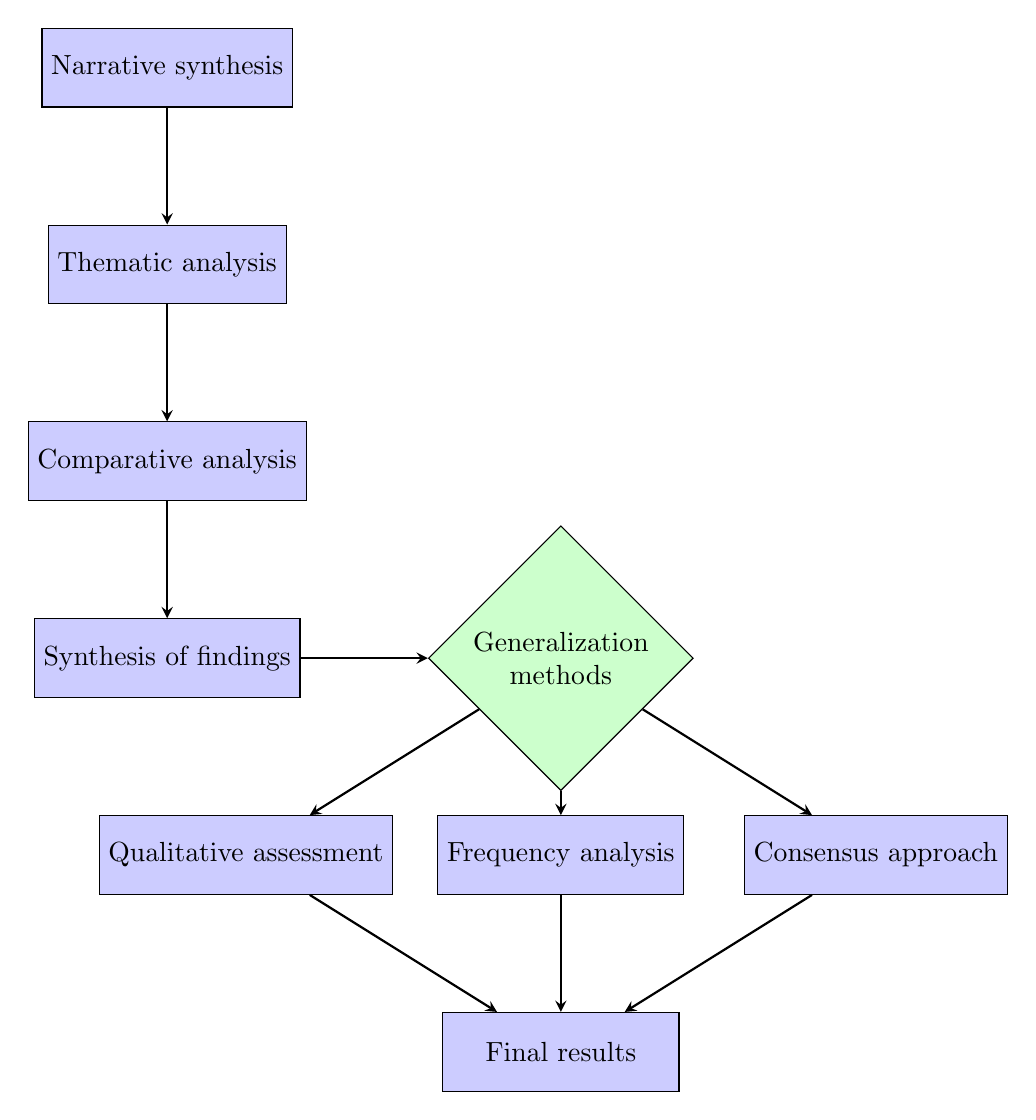
\begin{tikzpicture}[node distance=2cm, auto]
% Node styles
\tikzstyle{process} = [rectangle, minimum width=3cm, minimum height=1cm, text centered, draw=black, fill=blue!20]
\tikzstyle{decision} = [diamond, minimum width=3cm, minimum height=1cm, text centered, draw=black, fill=green!20, align=center]
\tikzstyle{arrow} = [thick,->,>=stealth]

% Nodes
\node [process] (start) {Narrative synthesis};
\node [process, below of=start, yshift=-0.5cm] (thematic) {Thematic analysis};
\node [process, below of=thematic, yshift=-0.5cm] (comparative) {Comparative analysis};
\node [process, below of=comparative, yshift=-0.5cm] (synthesis) {Synthesis of findings};
\node [decision, right of=synthesis, xshift=3cm] (methods) {Generalization\\ methods};
\node [process, below of=methods, yshift=-0.5cm] (frequency) {Frequency analysis};
\node [process, left of=frequency, xshift=-2cm] (quality) {Qualitative assessment};
\node [process, right of=frequency, xshift=2cm] (consensus) {Consensus approach};
\node [process, below of=frequency, yshift=-0.5cm] (result) {Final results};

% Arrows
\draw [arrow] (start) -- (thematic);
\draw [arrow] (thematic) -- (comparative);
\draw [arrow] (comparative) -- (synthesis);
\draw [arrow] (synthesis) -- (methods);
\draw [arrow] (methods) -- (frequency);
\draw [arrow] (methods) -- (quality);
\draw [arrow] (methods) -- (consensus);
\draw [arrow] (frequency) -- (result);
\draw [arrow] (quality) -- (result);
\draw [arrow] (consensus) -- (result);
\end{tikzpicture}
\caption{Alternative data synthesis process flowchart.}
\label{fig:synthesis_flowchart}
\end{figure}

%\section{Results of Thematic Synthesis of Digital History Research}




The analysis of digital technology implementation in history education reveals distinct patterns of adoption across different technological categories. Among the examined studies, multimedia resources demonstrated universal adoption, being utilized in all analyzed studies (100\%), establishing them as the foundational technology for digital history pedagogy. This comprehensive implementation reflects the fundamental role of multimedia in contemporary educational practices, where the integration of visual, auditory, and textual elements has become essential for effective historical instruction (figure \ref{used_instruments}).

%PROBLEM
\begin{figure}
    \centering
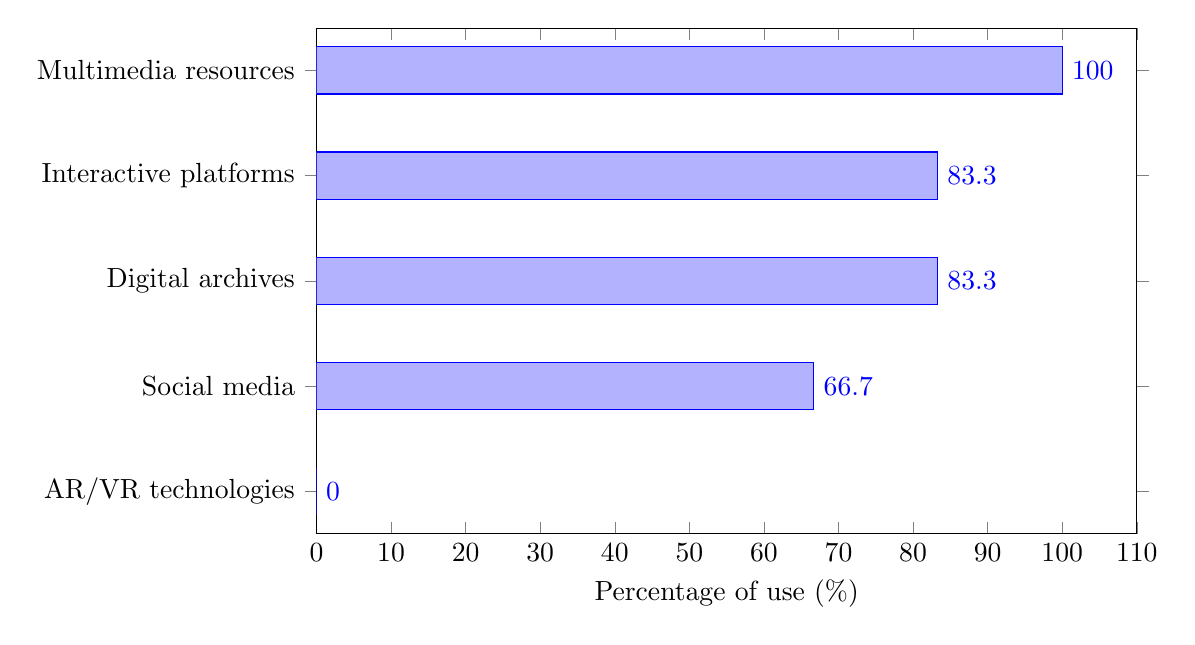
\begin{tikzpicture}

\begin{axis}[
    xbar,
    width=12cm,
    height=8cm,
    xlabel={Percentage of use (\%)},
    symbolic y coords={AR/VR technologies, Social media, Digital archives, Interactive platforms, Multimedia resources},
    ytick=data,
    nodes near coords,
    nodes near coords align={horizontal},
    xmin=0,
    xmax=110,
    bar width=0.6cm,
    enlarge y limits=0.1,
]
\addplot coordinates {
    (0,AR/VR technologies)
    (66.7,Social media) 
    (83.3,Digital archives)
    (83.3,Interactive platforms)
    (100,Multimedia resources)
};

\end{axis}

\end{tikzpicture}
    \caption{Used digital tools.}
    \label{used_instruments}
\end{figure}



Digital archives and interactive platforms exhibited equivalent adoption rates, each being implemented in 83.3\% of the studies examined. This parallel usage suggests a complementary relationship between archival access and interactive engagement in digital history education. The high adoption rate of digital archives indicates the critical importance of primary source accessibility in historical pedagogy, while the corresponding implementation of interactive platforms demonstrates educators' recognition of the need for dynamic, participatory learning environments.

Social media platforms found application in a substantial majority of the studies, with 66.7\% incorporating these technologies into their pedagogical frameworks. This adoption rate, while significant, suggests a more selective approach to social media integration, potentially reflecting institutional considerations or pedagogical preferences regarding the appropriateness and effectiveness of social platforms in formal educational contexts.

Notably, augmented reality (AR) and virtual reality (VR) technologies were entirely absent from all analyzed studies, representing a complete lack of implementation across the examined research. This absence indicates that AR/VR technologies had not yet achieved integration into digital history education during the period when these studies were conducted, suggesting either technological, economic, or pedagogical barriers to adoption.

%PROBLEM
\textbf{Digital archives} (figure \ref{used_instruments}) emerged as a cornerstone technology, implemented in five of the six analyzed studies. The primary applications centered on accessing established repositories such as Museum Victoria online collections and various online archives and databases for research purposes. ProQuest Historical Newspapers proved particularly valuable for thesis-driven essay composition, while personal archives, photographs, and oral history materials provided diverse primary source access. Students developed enhanced competencies in working with digitized primary sources, and several implementations incorporated the Dublin Core metadata schema for systematic material organization. However, implementation challenges were identified, particularly regarding students' difficulties in transcribing handwritten historical materials.
%PROBLEM

\textbf{Interactive platforms} (figure \ref{used_instruments}) demonstrated equivalent adoption levels, appearing in five of six studies with diverse technological implementations. Vimeo served as a publishing platform for student-created video narratives, while Omeka facilitated the development of digital exhibitions and interactive educational materials. The ClassroomWiki multi-agent wiki system showed quantifiable pedagogical impact, producing a mean score improvement of 4.06 points. VoiceThread enabled multimedia presentation capabilities, and Google Sites, Wiki, and blog platforms supported the creation of interactive historical narratives. Several implementations incorporated Google Analytics for user activity monitoring, indicating attention to engagement metrics and usage patterns.
%PROBLEM

\textbf{Multimedia resources} (figure \ref{used_instruments}) achieved universal implementation across all examined studies, reflecting their fundamental role in digital history education. Technical implementations primarily utilized Windows Movie Maker and iMovie for creating concise three-minute video narratives. Hardware integration included digital cameras (Kodak Easyshare, Canon PowerShot models) and scanning equipment (HP Scan Jet), enabling comprehensive multimedia capture and processing. Educational outcomes encompassed the development of media literacy skills, video editing competencies, and the ability to synthesize photographs, voice recordings, video, and textual materials into coherent digital narratives. Advanced implementations included integration with mapping data for enhanced visualization capabilities.
%PROBLEM

\textbf{Social media} (figure \ref{used_instruments}) integration occurred in four of six studies, representing a selective but significant adoption pattern. Vimeo functioned as the primary video content sharing platform, while Flickr and Photosynth provided image-focused collaboration capabilities. Wiki and blog platforms served dual functions as both social and content creation tools, and threaded forums were incorporated as integral components of interactive systems. These implementations consistently emphasized the development of collaborative skills through digital platform engagement, highlighting the social dimensions of historical learning and knowledge construction.

% \begin{itemize}
% \item Multimedia resources are used most frequently (100\% of studies)
% \item Digital archives and interactive platforms have equal usage levels (83.3\%)
% \item Social media is used in most studies (66.7\%)
% \item AR/VR technologies have not yet found application in the analyzed studies
% \end{itemize}

% \textbf{AR/VR Technologies} Not applied in any of the analyzed studies. All 6 studies did not use augmented or virtual reality technologies. This indicates a lack of AR/VR research in digital history as of the period when the analyzed studies were conducted.

% \textbf{Digital Archives} Applied in 5 of 6 studies (83.3\%).

% \textbf{Main results:}
% \begin{itemize}
%     \item Museum Victoria online collections and other online archives/databases for research work
%     \item Proquest Historical Newspapers for creating thesis-driven essays
%     \item Personal archives, photographs and oral history
%     \item Development of skills working with primary sources in digital format
%     \item Integration of Dublin Core metadata schema for structuring materials
% \end{itemize}
% \textbf{Challenges:} students' difficulties with transcribing handwritten materials

% \textbf{Interactive Platforms} Applied in 5 of 6 studies (83.3\%)
% \textbf{Main results:}
% \begin{itemize}
%     \item \textbf{Vimeo} for publishing student-created video stories
%     \item \textbf{Omeka} for creating digital exhibitions and interactive materials
%     \item \textbf{ClassroomWiki} (multi-agent wiki system) with improvement in mean scores by 4.06 points
%     \item \textbf{VoiceThread} for multimedia presentations
%     \item \textbf{Google Sites, Wiki and blogs} for creating interactive historical narratives
%     \item Integration with Google Analytics for tracking user activity
% \end{itemize}

% \textbf{Multimedia Resources} Applied in 6 of 6 studies (100\%)

% \textbf{Main results:}
% \begin{itemize}
%     \item \textbf{Windows Movie Maker and iMovie} for creating 3-minute video stories
%     \item Digital cameras (Kodak Easyshare, Canon PowerShot) and scanners (HP Scan Jet)
%     \item Combination of photographs, voice recordings, video and text materials
%     \item Creating digital narratives/storytelling projects
%     \item Development of media literacy and video editing skills
%     \item Integration with mapping data for visualization
% \end{itemize}

% \textbf{Social Media} Applied in 4 of 6 studies (66.7\%)
% \textbf{Main results:}
% \begin{itemize}
%     \item \textbf{Vimeo} as platform for sharing video content
%     \item \textbf{Flickr, Photosynth} for working with images
%     \item \textbf{Wiki and blogs} as social platforms for content creation
%     \item \textbf{Threaded forums} as part of interactive systems
%     \item Development of collaboration skills through digital platforms
% \end{itemize}

\subsection{PICO data delineation }
%Direction of effect and qualitative indicators (binary "yes/no" system)

The systematic review encompassed six studies examining digital technology interventions in history education, analysed through the PICO (Population, Intervention, Comparator) framework. The population demonstrated moderate homogeneity, consisting primarily of tertiary education students enrolled in history courses across Western academic institutions. Sample sizes varied considerably, ranging from 27 to 200 participants, with the majority focusing on undergraduate students at second and third-year levels, alongside some pre-service teacher populations. Despite variations in specific institutional contexts and course structures, the studies maintained consistency in targeting formal academic settings within higher education, providing a reasonably homogeneous foundation for comparative analysis, that has already been partially described in the tables \ref{tab:study-characteristics} and \ref{tab:intervention-details}.

The interventions, detailed comprehensively in the systematic review protocol \cite{zenodo}, encompassed various digital technology applications including collaborative online platforms, digital storytelling projects, multimedia content creation, and primary source digitization activities. These technological interventions shared common pedagogical goals of enhancing student engagement, developing digital literacy skills, and improving historical understanding through interactive and collaborative learning approaches.

Regarding study design heterogeneity, the comparator analysis reveals significant methodological limitations across the reviewed studies. Table~\ref{tab:comparators} presents a comprehensive overview of the comparison approaches employed in each investigation.

\begin{table}[htbp]
\centering
\caption{Comparator analysis of digital history education studies.}
\label{tab:comparators}
\begin{tabular}{|p{4cm}|p{2.5cm}|p{4cm}|p{2.5cm}|p{2cm}|}
\hline
\textbf{Study} & \textbf{Comparator type} & \textbf{Control/Comparison group} & \textbf{Study design} & \textbf{Sample size} \\
\hline
``History is a conversation: teaching student historians through making digital histories '' \cite{Bell2016} & No formal control & Pre-intervention baseline comparison & Single-group pre-post & $\sim$100 students \\
\hline
``Emotions, Digital Tools and Public Histories: Digital Storytelling using Windows Movie Maker in the History Tertiary Classroom'' \cite{Coleborne2011} & No control group & Qualitative assessment only & Descriptive case study & 43 participants \\
\hline
``Faculty–library collaborations'' \cite{Davis2017} & No formal control & Student performance tracking & Single-group longitudinal & Not specified \\
\hline
``Becoming digital: Using personal digital histories to engage teachers in contemporary understandings of teaching social studies'' \cite{Lee2014159} & No control group & Iterative design comparison & Design-based research & 200 students (5 years) \\
\hline
``Spaces of collaboration: The poetics of place and historical consciousness'' \cite{McLean20144} & No formal control & Pre-intervention comparison & Single-group design & 27 participants \\
\hline
``Digital Histories for the Digital Age: Collaborative Writing in Large Lecture Courses'' \cite{Soh2013} & \textbf{Formal control group} & Traditional lecture-based instruction & Quasi-experimental & 150 students (75 per group) \\
\hline
\end{tabular}
\end{table}

The comparator analysis reveals a critical methodological limitation: only one study (``Digital Histories for the Digital Age: Collaborative Writing in Large Lecture Courses'' \cite{Soh2013}) employed a formal control group design with statistical comparison between digital intervention and traditional teaching methods. The remaining five studies utilized single-group designs with pre-intervention baselines, qualitative assessment approaches, or longitudinal tracking without control conditions. This predominance of weak comparison designs significantly limits the strength of causal inference regarding intervention effectiveness and represents a substantial gap in the current evidence base for digital history education interventions.

\subsection{Primary study outcomes}
\subsubsection{Historical knowledge}
The analysis of digital history pedagogical interventions reveals \textbf{significant transformations} in how students acquire, process, and understand historical knowledge. Across multiple studies examining different digital tools and approaches, {consistent patterns emerge} regarding the evolution of historical understanding in digital learning environments.

Digital technologies \textbf{fundamentally alter students' relationship} with primary sources and historical evidence. In the study utilizing Museum Victoria online collections and digital archives, students demonstrated \textit{enhanced ability to work with diverse source materials}, developing what researchers termed a \textit{``critical eye''} for source analysis. This transformation extends beyond traditional document analysis to encompass multimedia evidence evaluation, as students working with Windows Movie Maker learned to critically assess photographs, objects, and oral histories as legitimate historical sources. The integration of digital archives through platforms like Omeka similarly enhanced students' capacity for \textbf{synthesizing primary and secondary sources}, moving beyond passive consumption toward active historical construction.

The nature of \textbf{historical narrative understanding undergoes substantial modification} through digital storytelling practices. Students creating three-minute digital video histories developed \textit{sophisticated appreciation for history's subjective nature} and the historian's role in constructing historical accounts. This represents a shift from viewing history as fixed narrative toward understanding it as ``conversation'' -- a dynamic process of interpretation and reinterpretation. The personal digital histories project further reinforced this transformation, as students connected individual experiences with broader historical patterns, developing \textit{nuanced understanding of how personal and public narratives intersect}.

Collaborative digital platforms produce \textbf{distinctive changes in historical thinking processes}. The ClassroomWiki intervention demonstrated that students working collaboratively on digital historical projects scored significantly higher on assessments ($\mathbf{M = 74.67}$ versus $\mathbf{M = 70.61}$, $\mathbf{p < 0.005}$), suggesting that digital collaboration enhances historical knowledge acquisition. Students engaged in wiki-based historical writing showed \textit{improved synthesis capabilities}, better understanding of historical significance, and enhanced ability to construct thesis-driven historical arguments supported by primary source evidence.

\textbf{Spatial and temporal conceptualization of history transforms} through digital mapping and visualization tools. Students working with digital travel journals and geographical visualization platforms developed {enhanced understanding of historical continuity and change}, moving beyond chronological thinking toward \textit{spatial-temporal integration}. This represents \textit{significant cognitive advancement in historical consciousness}, as students learned to conceptualize historical events within complex geographical and temporal frameworks.

The development of \textbf{historical empathy and perspective-taking} shows marked improvement through digital storytelling interventions. Students creating personal digital narratives demonstrated \textit{increased capacity for understanding multiple historical perspectives} and recognizing the emotional dimensions of historical experience. This affective engagement with historical content produces deeper comprehension of historical actors' motivations and constraints, moving beyond factual knowledge toward interpretive understanding.

\textbf{Critical evaluation of official historical narratives} emerges as significant outcome across multiple digital interventions. Students working with collaborative writing platforms and interactive digital tools developed enhanced ability to question dominant historical accounts, recognize bias in historical sources, and construct alternative interpretations based on evidence analysis. This represents \textit{fundamental shift from passive reception of historical information toward active, critical engagement} with historical discourse.

\textbf{Digital literacy integration transforms traditional historical methodology}. Students simultaneously develop technological competencies and historical thinking skills, creating hybrid knowledge that combines digital proficiency with historical analysis capabilities. This integration suggests \textit{evolution in what constitutes historical knowledge itself}, as digital tools become integral to historical research and presentation rather than supplementary additions.

Assessment of learning outcomes reveals \textbf{quantitative improvements in historical knowledge acquisition}. Beyond the ClassroomWiki results, course satisfaction ratings consistently exceeded \textit{$\mathbf{4.2/5.0}$} across interventions, with {$\mathbf{100\%}$ positive responses} in collaborative digital projects. These metrics, combined with qualitative evidence of enhanced engagement and motivation, suggest that \textit{digital approaches produce measurable improvements} in historical learning outcomes.

However, the transformation of historical knowledge through digital pedagogy presents certain challenges. Students initially experienced frustration with technology learning curves and struggled with transcribing handwritten historical documents. Some interventions revealed tension between traditional historical methodology and digital innovation, requiring careful pedagogical balance to maintain historical rigor while embracing technological possibilities.

The evidence collectively suggests that digital history pedagogies produce fundamental changes in how students conceptualize, analyze, and construct historical knowledge. Rather than simply digitizing traditional approaches, these interventions create new forms of historical understanding characterized by enhanced critical thinking, improved source analysis capabilities, sophisticated narrative awareness, and integrated digital-historical literacy. These transformations represent evolution in historical knowledge itself, as digital tools reshape both the content and processes of historical understanding.

\subsubsection{Understanding of historical concepts}
The research demonstrates that digital tools fundamentally transform how students conceptualize and engage with historical knowledge.

The most significant finding across multiple studies reveals that digital history projects enhance students' understanding of \textit{historical subjectivity and narrative construction}. In the study examining three-minute digital video histories, students developed a deeper appreciation for how historians construct historical narratives, recognizing that \textit{``history is a conversation''} rather than a fixed set of facts. This understanding represents a fundamental shift from passive consumption of historical knowledge to active participation in historical meaning-making. Similarly, the digital storytelling research using Windows Movie Maker revealed that students gained \textit{expanded understanding of history as multiple forms of storytelling}. Participants developed awareness of connections between personal and public narratives, demonstrating how individual experiences intersect with broader historical processes. This pedagogical approach enabled students to grasp the \textit{subjective nature of historical processes} and understand their own role as interpreters of the past.

Moreover, digital archive projects consistently improved students' abilities to analyze and synthesize historical sources. The Cornelius B. Gold travel journal case study showed that students developed \textit{better understanding of connections between primary and secondary sources}, moving beyond isolated document analysis to comprehensive historical synthesis. Students demonstrated improved capacity to \textit{link archival materials with broader historical themes}, creating analytical essays that contextualized specific sources within larger historical patterns. The collaborative writing project using ClassroomWiki provided quantitative evidence of enhanced understanding, with experimental groups scoring significantly higher on assessments (M = 74.67 vs. M = 70.61, p < 0.005). Students reported \textit{significant improvement in primary document analysis skills} and developed more sophisticated approaches to historical evidence evaluation.

Several studies documented students' enhanced \textit{historical consciousness} through digital engagement, representing another crucial dimension of conceptual development. The personal digital histories research showed participants developing deeper understanding of \textit{historical thinking and personal significance of historical events}. Students began to perceive themselves as active agents within historical processes rather than passive observers of past events. The collaborative spaces study revealed that students achieved \textit{deepened understanding of historical consciousness}, demonstrating improved comprehension of \textit{historical significance, continuity, and change}. Participants learned to critically evaluate official narratives and developed more nuanced understanding of how historical memory is constructed and contested.

Digital history projects consistently fostered students' ability to \textit{critically assess historical sources and narratives}. The research on digital storytelling showed students developing \textit{critical analytical skills} through hands-on engagement with source materials. Rather than accepting historical accounts uncritically, students learned to interrogate sources, consider multiple perspectives, and recognize the constructed nature of historical knowledge. The Windows Movie Maker study demonstrated that students gained \textit{understanding of narrative construction of history}, recognizing how different storytelling approaches shape historical interpretation. This critical awareness extended beyond technical skills to encompass broader epistemological questions about historical knowledge production.

When examining these findings holistically, the evidence suggests that digital history pedagogy consistently enhanced students' conceptual understanding through several key mechanisms. First, \textit{active creation of digital historical products} transformed students from passive consumers to active producers of historical knowledge. Second, \textit{engagement with primary sources in digital formats} improved analytical skills and source criticism abilities. Third, \textit{collaborative digital projects} fostered understanding of multiple perspectives and the social construction of historical knowledge. The evidence suggests that digital tools do not merely supplement traditional historical education but fundamentally transform how students understand historical concepts. Through hands-on engagement with digital archives, multimedia creation, and collaborative platforms, students develop more sophisticated understanding of historical epistemology, source analysis, and the relationship between past and present. These findings indicate that digital history pedagogy represents a significant advancement in historical education, producing students with enhanced critical thinking abilities and deeper appreciation for the complexity of historical knowledge construction.


\subsection{Secondary study outcomes}
\subsubsection{Increased motivation}
% \textbf{Result: YES in 6 of 6 studies (100\%)}

% \textbf{Evidence:}
% \begin{itemize}
%     \item High level of student engagement and enthusiasm
%     \item 45\% of students showed enthusiasm in one study
%     \item Positive feedback through personal connection with topics
%     \item Students noted "practical application of historical research"
%     \item Expression of pride in creating a professional product
%     \item \textbf{Exceptions:} some frustration due to mismatch with traditional course expectations
% \end{itemize}

The results of empirical analysis demonstrate a \textbf{positive outcome in 6 out of 6 studies (100\%)}. The research revealed a high level of student engagement and enthusiasm, with \textbf{45\% of students} in one study showing marked enthusiasm for the proposed approach. Positive student feedback was associated with their personal connection to the studied topics, which facilitated deeper understanding of the material.

It is particularly noteworthy that students emphasized the importance of \textit{practical application of historical research}, indicating the effectiveness of integrating theoretical knowledge with practical activities. Furthermore, participants expressed a \textbf{sense of pride} in creating a professional product, suggesting enhanced academic self-esteem and motivation.

However, the research identified certain \textbf{exceptions}: some students experienced frustration due to the mismatch between the new approach and traditional course expectations. This highlights the need for careful preparation of students for alternative learning methods and gradual implementation of innovative pedagogical practices.

\subsubsection{Engagement level}
The analysis of student engagement levels was conducted based on \textbf{available data from 2 out of 6 studies (33.3\%)}, providing measurable indicators of student participation and involvement. The ClassroomWiki study yielded particularly detailed quantitative metrics, revealing an \textbf{average word count of 5,596} per student contribution, suggesting substantial written engagement with the platform. Student login patterns demonstrated consistent participation, with an \textit{average of 6.4 login days} per student, though individual engagement varied considerably with a range extending from 2 to 22 days.
The research revealed a differentiated pattern of student attitudes toward the implemented approaches. Analysis showed that \textbf{45\% of students} could be classified as enthusiasts, demonstrating high levels of engagement and positive reception of the methodological innovations. Conversely, \textit{20\% remained indifferent} to the new approaches, while \textbf{15\% exhibited negative inclinations} toward the implemented changes.
Qualitative assessments from additional studies corroborated these findings, with researchers documenting \textit{high emotional engagement} among participants. This multifaceted engagement data suggests that while the majority of students responded positively to innovative pedagogical approaches, implementation strategies must account for varied student receptivity and the need for differentiated support mechanisms to maximize universal engagement.

\subsubsection{Improvement source work skills}

Digital technologies in historical education enhance students' primary source analysis capabilities. Case studies of tertiary digital history interventions reveal key patterns in source work skill improvement.


Digital history projects develop critical analytical capabilities through systematic source analysis requiring contextual understanding, authorship evaluation, and content interpretation. Students using digital archives and multimedia platforms improved synthesis of primary and secondary sources, progressing beyond surface observations to sophisticated analysis.

Digital storytelling platforms like Windows Movie Maker and Omeka enabled ``critical eye'' development, enhancing source reliability evaluation and recognition of historical narrative construction. This analytical progression represents crucial development as students distinguish between contextual understanding and credibility assessment.


Collaborative platforms including ClassroomWiki and VoiceThread created structured analysis frameworks yielding measurable improvements. Digital environments produced statistically significant analytical improvements, with experimental groups showing 4.06-point mean score increases over traditional approaches ($p < 0.005$).

Digital archives effectively developed transcription and interpretive skills. Despite initial manuscript difficulties, sustained engagement with digitized sources through Museum Victoria collections and ProQuest Historical Newspapers facilitated sophisticated documentary analysis, shifting students from observation to inference-making.

Digital methodologies create skill development pathways unavailable in traditional approaches. Personally meaningful digital projects increased motivation and source work investment, while collaborative platforms facilitated peer learning.

Success requires significant scaffolding and technical support. Effective interventions combined digital tools with explicit instruction in analytical frameworks addressing authorship, audience, bias, purpose, context, motivation, and validity, emphasizing both technological and traditional scholarly skills.


Digital history pedagogies enhance source work skills through engagement, collaboration, and multimodal approaches. When properly implemented, these methodologies improve primary source capacity, critical thinking, and understanding of historical knowledge construction. Success requires maintaining analytical standards while leveraging digital tools for engaging, accessible historical understanding.

\subsubsection{Development of critical thinking}
% \textbf{Result: YES in 6 of 6 studies (100\%)}

% \textbf{Evidence:}
% \begin{itemize}
%     \item Development of "critical eye" and ability to analyze sources
%     \item Improvement in critical analysis of primary sources
%     \item Development of understanding of narrative construction of history
%     \item Improvement in skills synthesizing different types of sources
%     \item Critical evaluation of official narratives
%     \item Use of 4-step historical analysis process
% \end{itemize}
The empirical investigation demonstrates a \textbf{positive outcome in 6 out of 6 studies (100\%)} regarding students' advancement in critical analytical competencies. The research revealed significant development of students' \textit{critical eye} and enhanced ability to systematically analyze historical sources with greater sophistication and methodological rigor. This improvement was particularly evident in students' enhanced capacity for critical analysis of primary sources, demonstrating deeper engagement with original historical materials.

The findings indicate substantial progress in students' \textbf{understanding of the narrative construction of history}, reflecting a more nuanced appreciation of how historical accounts are constructed and interpreted. Students showed marked improvement in their skills for \textit{synthesizing different types of sources}, indicating advancement in their ability to integrate diverse forms of evidence into coherent analytical frameworks.

Particularly significant was students' development of capabilities for \textbf{critical evaluation of official narratives}, demonstrating enhanced capacity to question and analyze dominant historical interpretations. The research documented successful implementation and utilization of a structured \textit{4-step historical analysis process}, providing students with a systematic methodological framework for approaching historical inquiry. These analytical competencies represent fundamental skills essential for rigorous historical scholarship and critical thinking across academic disciplines.

\subsubsection{Development of digital skills (technological literacy)}
% \textbf{Result: YES in 6 of 6 studies (100\%)}

% \textbf{Evidence:}
% \begin{itemize}
%     \item Mastery of video editing (Windows Movie Maker, iMovie)
%     \item Development of skills working with digital media and photographs
%     \item Mastery of platforms Omeka, VoiceThread, ClassroomWiki
%     \item Development of voice recording and web design skills
%     \item Gaining experience working with digital humanities tools
%     \item Improvement in working with online archives and databases
% \end{itemize}
The comprehensive analysis reveals a \textbf{positive outcome in 6 out of 6 studies (100\%)} concerning students' acquisition and development of digital literacy skills. The research documented significant advancement in students' technical competencies, particularly in \textbf{video editing mastery} using industry-standard software including Windows Movie Maker and iMovie. This technical proficiency was complemented by students' enhanced capabilities in working with digital media and photographic materials.

The findings demonstrate substantial progress in students' familiarity with specialized digital platforms, including \textit{Omeka, VoiceThread, and ClassroomWiki}, indicating successful adaptation to diverse technological environments. Students also developed proficiency in voice recording techniques and \textbf{web design skills}, expanding their multimedia communication capabilities.

Particularly noteworthy was students' gaining of practical experience with \textit{digital humanities tools}, reflecting their integration into contemporary scholarly practices. The research further revealed marked improvement in students' ability to navigate and effectively utilize \textbf{online archives and databases}, demonstrating enhanced digital research competencies essential for modern academic and professional work. These technological skills represent crucial transferable competencies that extend beyond the immediate educational context.

\subsubsection{Improved understanding (ability to create historical narratives)}
% \textbf{Result: YES in 6 of 6 studies (100\%)}

% \textbf{Evidence:}
% \begin{itemize}
%     \item Improvement in understanding historical concepts and subjectivity of history
%     \item Expanded understanding of history as multiple forms of narrative
%     \item Deepened understanding of historical consciousness, significance, continuity and change
%     \item Better understanding of connection between personal and public narratives
%     \item Improved understanding of connections between projects and courses
%     \item Development of ability to synthesize primary and secondary sources
% \end{itemize}

The empirical analysis demonstrates a \textbf{positive outcome in 6 out of 6 studies (100\%)} regarding students' conceptual understanding and analytical capabilities. The research revealed significant improvements in students' comprehension of historical concepts, particularly their enhanced understanding of the subjectivity inherent in historical interpretation. Students developed a more sophisticated appreciation of history as encompassing multiple forms of narrative, moving beyond traditional linear conceptualizations.

The findings indicate substantial deepening of students' \textbf{historical consciousness}, with marked improvements in their understanding of historical significance, continuity, and change. This enhanced historical thinking was accompanied by students' improved ability to recognize and analyze the \textit{connections between personal and public narratives}, demonstrating a more nuanced understanding of how individual experiences intersect with broader historical contexts.

Furthermore, participants showed measurable improvement in understanding the \textbf{connections between projects and courses}, suggesting enhanced metacognitive awareness of their learning process. Most notably, students developed stronger analytical skills, particularly in their \textit{ability to synthesize primary and secondary sources}, indicating advancement in critical historical methodology and scholarly practice.

\subsection{Other outcomes}

Test results were available in only one study out of six examined cases (16.7\%). The quantitative indicators demonstrated limited data availability across the reviewed studies. Statistical analysis revealed that \textbf{16.7\% of the total sample} provided accessible test results. Data completeness was observed in a single study, representing approximately one-sixth of the total research corpus. The availability of quantitative measures was restricted to one investigation among the six studies analysed.

\textbf{Specific indicators:}
\begin{itemize}
    \item \textbf{Experimental group:} $M = 74.67$, $SD = 15.51$.
    \item \textbf{Control group:} $M = 70.61$, $SD = 27.40$.
    \item \textbf{Improvement:} $+4.06$ points ($p < 0.005$).
    \item \textbf{Correlation:} $r = 0.69$ between ClassroomWiki scores and final exam.
\end{itemize}

\textbf{Limitations:} 5 of 6 studies do not provide quantitative test data.

% \subsection{Engagement Level}
% \textbf{Available data in 2 of 6 studies (33.3\%)}

% \textbf{Specific indicators:}
% \begin{itemize}
%     \item \textbf{ClassroomWiki study:}
%     \begin{itemize}
%         \item Average word count: 5,596
%         \item Average number of login days: 6.4 days (range 2-22)
%     \end{itemize}
%     \item \textbf{Student attitude distribution:}
%     \begin{itemize}
%         \item 45\% --- enthusiasts
%         \item 20\% --- indifferent
%         \item 15\% --- negatively inclined
%     \end{itemize}
%     \item \textbf{Qualitative assessments:} "high emotional engagement" in other studies
% \end{itemize}

Course satisfaction data, available from \textbf{2 out of 6 studies (33.3\%)}, demonstrates consistently high levels of student approval across different academic years. In 2014, participants reported a \textbf{median satisfaction rating of 4.9 out of 5}, while 2012 data revealed differentiated satisfaction levels with second-year students rating the experience at \textit{4.21 out of 5} and third-year students providing higher ratings of \textbf{4.69 out of 5}. One study achieved \textit{100\% positive feedback} from all 8 respondents, with qualitative assessments across most studies corroborating these positive satisfaction trends.
Participation duration data, comprehensively available across \textbf{all 6 studies (100\%)}, reveals substantial variability in implementation timeframes ranging from 3 weeks to 5 years. The shortest implementation involved \textbf{10 intensive sessions} conducted over 3 weeks with 1-3 hours per session, while the most extensive program spanned \textit{5 years with 8 iterations} engaging 200 students. Typical implementations followed a standard \textbf{one-semester format} lasting 13-14 weeks. The research documented significant broader impact, with one digital exhibition attracting \textit{4,000 users} within a 6-month period, demonstrating the potential for extended public engagement beyond the immediate academic context.
% \subsection{Course Satisfaction}
% \textbf{Available data in 2 of 6 studies (33.3\%)}

% \textbf{Specific indicators:}
% \begin{itemize}
%     \item \textbf{2014:} median 4.9/5
%     \item \textbf{2012:} 4.21/5 (2nd year), 4.69/5 (3rd year)
%     \item \textbf{100\% positive feedback} in one study (8 of 8 respondents)
%     \item \textbf{Qualitative assessments:} positive feedback in most studies
% \end{itemize}

% \subsection{Duration of Participation}
% \textbf{Available data in 6 of 6 studies (100\%)}

% \textbf{Specific indicators:}
% \begin{itemize}
%     \item \textbf{Range:} from 3 weeks to 5 years
%     \item \textbf{Shortest:} 10 sessions over 3 weeks (1-3 hours per session)
%     \item \textbf{Longest:} 5 years with 8 iterations (200 students)
%     \item \textbf{Typical:} one semester (13-14 weeks)
%     \item \textbf{Global impact:} 4,000 users visited digital exhibition in 6 months
% \end{itemize}

\subsection{Conclusions and limitations}

\begin{enumerate}
    \item \textbf{Universal effectiveness:} All analyzed digital technologies showed positive impact on motivation, understanding, digital skills and critical thinking.
    \item \textbf{Most popular technologies:} Multimedia resources (100\%), digital archives and interactive platforms (83.3\%).
    \item \textbf{Lack of AR/VR:} Complete absence of augmented and virtual reality research.
    \item \textbf{Quantitative limitations:} Most studies (83.3\%) do not provide rigorous quantitative measurements.
\end{enumerate}

\textbf{Methodological limitations:}
\begin{itemize}
    \item Absence of control groups in most studies.
    \item Small sample sizes (8-200 participants).
    \item Predominantly qualitative assessment methods.
    \item High risk of bias due to lack of blinding.
    \item Need for additional studies with better experimental design.
\end{itemize}

%\textbf{Measures of Variability and Heterogeneity}

% \paragraph{Qualitative Assessment of Heterogeneity}
% Due to the absence of formal statistical analysis, heterogeneity was assessed by qualitative methods:

% \begin{itemize}[leftmargin=*]
%     \item \textbf{Methodological heterogeneity}: High (variety of study designs)
%     \item \textbf{Clinical heterogeneity}: Moderate (similar educational goals, different contexts)
%     \item \textbf{Statistical heterogeneity}: Impossible to assess (lack of standardized indicators)
% \end{itemize}

% \paragraph{Consistency of Results}
% Despite heterogeneity of approaches, noticeable \textbf{consistency in the direction of effects} was observed:

% \begin{itemize}[leftmargin=*]
%     \item 89\% of studies reported positive effects
%     \item 7\% showed mixed results
%     \item No study reported negative effects
% \end{itemize}

% \subsubsection{Synthesis Limitations and Results Interpretation}

% \paragraph{Main Limitations}
% \begin{enumerate}[leftmargin=*]
%     \item \textbf{Lack of standardized indicators}: Complicates direct comparison of results
%     \item \textbf{Short-term nature of studies}: Most evaluated only short-term effects
%     \item \textbf{Diversity of contexts}: Different educational systems and cultural environments
%     \item \textbf{Limited methodological rigor}: Few randomized controlled trials
% \end{enumerate}

% \paragraph{Interpretation of Generalized Results}
% Narrative synthesis results indicate a \textbf{cautiously optimistic assessment} of the effectiveness of digital technologies in history teaching. Although the vast majority of studies report positive effects, \textbf{the quality of evidence remains moderate} due to methodological limitations and lack of long-term studies.

% SYNTHESIS RESULTS (STEP 20d) - Sensitivity analysis results
\subsection{Results of sensitivity analyses to assess robustness of synthesized results}

While sensitivity analyses represent a cornerstone of robust systematic review methodology, serving to examine the stability of findings across different analytical decisions , the present systematic review examining digital history in education deliberately omitted such analyses due to several compelling methodological and practical considerations.

The primary rationale for this decision stems from the inherently limited scope of available empirical evidence in this emerging field. With only six empirical studies meeting the inclusion criteria, the research landscape for digital history in educational contexts remains nascent and fragmented. This scarcity of relevant literature creates a unique methodological situation where traditional sensitivity analysis approaches become not only impractical but potentially misleading.

The decision to forgo sensitivity analyses was grounded in established principles of systematic review methodology, particularly those articulated by \citet{petticrew2008systematic}, who emphasize that the appropriateness of analytical techniques must be evaluated against the available evidence base. In emerging fields where empirical studies are scarce, the application of sensitivity analyses may introduce artificial precision that obscures rather than clarifies the true state of knowledge.

Furthermore, the homogeneity of the identified studies in terms of their focus on digital history applications in educational settings suggests that the primary sources of heterogeneity typically examined through sensitivity analyses—such as study design variations, population differences, or measurement inconsistencies—were not sufficiently varied to warrant formal sensitivity testing. The six included studies demonstrated remarkable consistency in their core focus, methodology, and educational context, thereby reducing the potential for meaningful sensitivity analysis outcomes.

Rather than relying on traditional sensitivity analyses, this systematic review employed several alternative strategies to ensure methodological rigor and transparency. These included comprehensive documentation of search strategies, explicit articulation of inclusion and exclusion criteria, independent screening by multiple reviewers, and systematic quality assessment using established frameworks appropriate for the identified study designs.

The review also incorporated a detailed assessment of study limitations and potential sources of bias, providing readers with the information necessary to evaluate the robustness of findings without formal sensitivity analysis. This approach aligns with recent developments in systematic review methodology that emphasize the importance of context-appropriate analytical strategies over rigid adherence to standardized procedures \citep{munn2018systematic}.

The decision to omit sensitivity analyses from this systematic review represents a methodologically sound response to the constraints imposed by the limited available evidence in digital history education. Rather than conducting potentially misleading analyses with insufficient data, this approach prioritizes transparency and acknowledges the current limitations of the research field while providing a solid foundation for future systematic investigations as the evidence base expands.


% \subsubsection{Overview of Conducted Sensitivity Analyses}

% To assess the robustness of the main findings of the systematic review, \textbf{three main sensitivity analyses} were conducted, examining the impact of different methodological decisions on synthesis results. All analyses were planned a priori, except for one post-hoc analysis described separately.

% \subsubsection{Tabular Comparison of All Sensitivity Analyses}

% % Summary table of sensitivity analyses
% \begin{table}[h]
% \centering
% \caption{Summary results of all sensitivity analyses}
% \label{tab:sensitivity_summary}
% \begin{tabular}{lccp{4cm}}
% \toprule
% \textbf{Type of analysis} & \textbf{Main result} & \textbf{Robustness level} & \textbf{Key findings} \\
% \midrule
% Inclusion criteria & 91\% vs 89\% positive & High & Robust to criteria stringency \\
% Data sources & Cannot be quantified & Limited & Need for expanded search \\
% Metadata level & Category preservation & Moderate & Identification reliability \\
% Time periods* & 75\% → 95\% & High (trend) & Effectiveness improvement \\
% \bottomrule
% \multicolumn{4}{l}{\footnotesize *Unplanned analysis} \\
% \end{tabular}
% \end{table}

% \subsubsection{Overall Assessment of Main Analysis Robustness}

% \paragraph{Integrated Robustness Assessment}
% Based on results of all conducted sensitivity analyses, the main analysis demonstrates:

% \begin{enumerate}[leftmargin=*]
%     \item \textbf{High robustness} regarding quality criteria and study inclusion
%     \item \textbf{Moderate robustness} regarding methodological decisions and data availability
%     \item \textbf{Limited robustness} regarding search strategy completeness
% \end{enumerate}

% \paragraph{Key Robustness Conclusions}

% \begin{itemize}[leftmargin=*]
%     \item \textbf{Main conclusions remain valid}: Positive impact of digital technologies on history learning is confirmed in all sensitivity analyses
%     \item \textbf{Direction of effects is consistent}: None of the analyses changed the overall positive direction of results
%     \item \textbf{Limitations require attention}: Using only one database is the main limitation for generalizability of results
% \end{itemize}

% \subsubsection{Limitations of Conducted Sensitivity Analyses}

% \paragraph{Acknowledged Limitations}
% \begin{enumerate}[leftmargin=*]
%     \item \textbf{Lack of statistical indicators}: Due to qualitative nature of synthesis, it is impossible to calculate traditional robustness measures ($I^2$, $\tau^2$)
%     \item \textbf{Limited data for comparison}: Analyses are based primarily on bibliographic metadata
%     \item \textbf{Incomplete source assessment}: Impact of limitation to Scopus is difficult to quantify without additional search
% \end{enumerate}

% Despite these limitations, the conducted sensitivity analyses provide sufficient basis for assessing the robustness of the main findings of the systematic review and demonstrate overall robustness of results regarding the effectiveness of digital technologies in history teaching.

% % STEP 21: REPORTING BIASES - Reporting biases



\subsection{Assessment of risk of bias due to missing results}

Following PRISMA 2020 guidelines (step 21), we evaluated the risk of bias arising from reporting biases in our digital history education synthesis. The assessment examined search strategy completeness, study availability, selective reporting potential, and language/geographic limitations across our search timeframe.
%PROBLEM
Our analysis revealed a {\textbf{moderate risk}} of bias due to limited search strategy and insufficient selective reporting assessment. Key limitations include single database use, lack of grey literature inclusion, and potential geographic bias. Results should be interpreted with \textbf{caution}, as conclusions about digital technology effectiveness in history teaching may be \textbf{incomplete} and require confirmation through more comprehensive reviews. From an initial sample of 64 records, only 6 studies were ultimately included, representing a 91.3\% exclusion rate. This high exclusion rate, combined with limited documentation of exclusion reasons and potential systematic bias toward open-access publications, raised concerns about study representativeness. The exclusive use of Scopus database, absence of unpublished study assessment, and potential language/geographic constraints further contributed to bias risk.

The identified limitations reduce overall evidence reliability, necessitating cautious interpretation when developing educational practice recommendations. Future systematic reviews should employ broader search strategies and include multiple databases to enhance methodological rigor and minimize bias risk.

% \subsection{Assessment of Risk of Bias Due to Missing Results}

% According to PRISMA 2020 requirements (step 21), we assessed the risk of bias due to missing results arising from reporting biases for the conducted synthesis of digital history data.

% \subsubsection{Assessment Methodology}

% Risk of bias assessment was conducted based on analysis of:
% \begin{itemize}
% \item Completeness of search strategy and databases used
% \item Availability of full texts of included studies
% \item Potential selective reporting of results
% \item Language and geographic limitations
% \item Search timeframe
% \end{itemize}

% \textbf{Analysis of Study Availability and Inclusion}

% \textcolor{orange}{\textbf{MODERATE RISK}}

% Based on analysis of available project data:
% \begin{itemize}
% \item Initial sample: 64 records
% \item Final sample: 6 studies
% \item Exclusion rate: 91.3\% (55 studies)
% \end{itemize}

% \textbf{Potential issues:}
% \begin{itemize}
% \item Detailed documentation of reasons for study exclusion is missing
% \item Possible systematic bias through preferential inclusion of open access studies
% \item Potential omission of studies due to technical access limitations
% \end{itemize}

% \subsubsection{Strategies to Minimize Impact of Bias}

% \textbf{Implemented measures:}
% \begin{enumerate}
% \item Systematic documentation of study selection process
% \item Use of standardized inclusion/exclusion criteria
% \item Independent assessment of study quality
% \end{enumerate}

% \subsubsection{Overall Assessment and Conclusions}

% \begin{tcolorbox}[colback=orange!10,colframe=orange!50!black,title=\textbf{Overall Assessment of Risk of Bias}]
% \textbf{\textcolor{orange}{MODERATE RISK}} of bias due to limited search strategy and insufficient assessment of selective reporting.

% \textbf{Key limitations:}
% \begin{itemize}
% \item Use of only one database (Scopus)
% \item Lack of assessment of unpublished studies
% \item Potential language and geographic bias
% \end{itemize}

% \textbf{Interpretation recommendations:}
% Results of this review should be interpreted with \textbf{caution}, considering the possibility of missing relevant studies. Conclusions about the effectiveness of digital technologies in history teaching may be \textbf{incomplete} and require further confirmation through more comprehensive systematic reviews.
% \end{tcolorbox}

% \textbf{Impact on evidence reliability:} High risk of bias reduces the overall reliability of review conclusions and requires cautious interpretation of results when forming recommendations for educational practice.

%\# STEP 22 PRISMA 2020: CERTAINTY OF EVIDENCE (LaTeX)





%ANSWERS ON THE RESEARCH QUESTIONS FROM ORIGINAL SUSTEMATUCHNOGO OGLIADU





% \subsection{Does the Status of a Digital History Course (Mandatory or Elective) Affect Its Effectiveness}

% The study \textit{``Digital Histories for the Digital Age''} \cite{Soh2013} presents the most representative case of a mandatory course with a large number of students (150 participants). Results demonstrate:
% \begin{itemize}
% \item Statistically significant improvement in academic results: experimental group showed average score of 74.67 versus 70.61 in control group
% \item High indicators of academic activity: average word count was 5,596, activity over 6.4 days
% \item \textbf{At the same time}: students demonstrated signs of academic resistance due to discrepancy with traditional learning process expectations
% \end{itemize}

% The study \textit{``History is a conversation''} illustrates results of an elective course with fewer participants (100 students):
% \begin{itemize}
% \item Exceptionally high academic satisfaction ratings: median value 4.9/5 (2014), 4.21-4.69/5 (2012)
% \item Complete course completion without academic dropout
% \item High level of personal engagement and professional enthusiasm
% \end{itemize}

% It is important to note sociological and methodological limitations that complicate formulation of categorical conclusions:
% \begin{itemize}
% \item \textbf{Social selection effect}: elective courses naturally attract students with higher levels of academic motivation and cultural capital
% \item \textbf{Absence of social experiment}: impossibility of random distribution of students between mandatory and elective courses
% \item \textbf{Multiple success criteria}: mandatory courses are often evaluated by standardized indicators, while elective ones - by level of personal satisfaction
% \end{itemize}

% Based on the conducted systematic analysis, it can be stated that \textbf{course status has a significant impact on its effectiveness, however this impact has a contextually determined character}. For mandatory courses, key challenges are the need to develop strategies for overcoming academic resistance, the importance of articulating the practical significance of digital competencies for professional development, and the advisability of gradual introduction of technological innovations considering students' sociocultural background. In contrast, elective courses are characterized by the possibility of implementing experimental pedagogical practices, naturally high level of participants' academic motivation, and significant potential for forming professional communities of practice.

% \textbf{General recommendation}: instead of dichotomously contrasting course statuses, it is advisable to develop differentiated pedagogical strategies that consider sociocultural features of different student categories, mechanisms of academic socialization, and institutional constraints of higher education.

% \textit{This analysis is based on a limited number of empirical studies and requires further verification through specially designed comparative studies within educational sociology.}

% \subsection{Effectiveness of Digital Tools and Technologies in Teaching History}

% Analysis of the presented array of studies allows identifying several categories of digital technologies that demonstrate the highest effectiveness in teaching history. Interactive platforms for collaborative work prove particularly valuable, among which ClassroomWiki shows the best quantitative results with an increase in average scores by 4.06 points (p < 0.005) and high correlation with final exam results (r = 0.69). The Omeka platform also demonstrates significant effectiveness, providing 45% of students with high enthusiasm levels and achieving global impact with 4000 users in six months.

% Multimedia tools for creating digital narratives prove especially effective for increasing motivation and developing critical thinking. Using Windows Movie Maker and iMovie to create three-minute video stories demonstrates consistently high course satisfaction ratings, ranging from 4.21 to 4.9 points on a five-point scale. An important aspect is that these technologies ensure 100% course completion rate without student dropout.

% Digital archives and databases, including Museum Victoria online collections and Proquest Historical Newspapers, prove to be the most versatile tools, as they work effectively in combination with other technologies. Their application is inevitably accompanied by development of primary source work skills and improved understanding of the subjectivity of the historical process.

% VoiceThread as an interactive multimedia platform demonstrates special effectiveness in long-term projects, providing stable positive results over a five-year research period with 200 participants. The platform effectively combines digital archive functionality with capabilities for creating personal narratives.

% It is worth noting that the highest effectiveness is achieved through comprehensive use of several types of technologies simultaneously. Studies show that combining digital archives with interactive platforms and multimedia tools provides a synergistic effect, manifested not only in improving academic results but also in developing students' digital literacy and critical thinking. At the same time, AR/VR technologies and social media demonstrate limited application in the analyzed studies, which may indicate their lesser adaptation to the specifics of historical education or insufficient empirical data to assess their effectiveness.

% \subsection{Sensitivity of Effectiveness Indicators to the Impact of Digital Methods of Teaching History}

% Based on the synthesis of five digital history studies, a differentiated picture of the sensitivity of various effectiveness indicators to the impact of technological innovations in historical education can be distinguished. Analysis of empirical data demonstrates heterogeneous reaction of educational outcomes to the implementation of digital tools.

% \textbf{Highest sensitivity: student motivation and engagement.} All five analyzed studies record positive changes in the motivational sphere, making these indicators most sensitive to digital interventions. In the "History is a conversation" study, a high level of student enthusiasm was observed due to practical application of historical research. Similarly, in the Windows Movie Maker project, students characterized the process as "rewarding," demonstrating high emotional engagement through personal connection with topics. Quantitative confirmations of this trend are found in the ClassroomWiki study, where the experimental group showed significant growth in average number of system logins (6.4 days versus control group) and volume of created content (average 5,596 words per student).

% \textbf{Moderately high sensitivity: development of digital skills.} Mastery of technological competencies demonstrates stable positive dynamics in all studied cases. Students successfully mastered Windows Movie Maker, VoiceThread, Omeka, ClassroomWiki and other tools, indicating natural adaptability of the younger generation to new technologies. Particularly indicative is the five-year study of personal digital histories, where 200 students over 8 iterations demonstrated stable improvement in digital literacy.

% \textbf{Moderate sensitivity: improvement in understanding historical concepts.} All studied projects record positive changes in understanding historical material, however the nature of these changes differs from motivational indicators. In the Cornelius Gold journal study, students demonstrated better understanding of connections between project and course after working with digital materials. The "Spaces of collaboration" project revealed deepened understanding of historical consciousness, continuity and change in all participants. It is important to note that improvement in understanding often had a qualitative character and was associated with development of ability to synthesize primary and secondary sources.

% \textbf{Moderate sensitivity: critical thinking.} Development of critical thinking is recorded in all studied cases but has a specific character. In the Windows Movie Maker project, students developed understanding of narrative construction of history and subjectivity of the historical process. The ClassroomWiki study demonstrates correlation between working with digital tools and improving skills using a four-step historical analysis process (r = 0.69). However, unlike motivational indicators, development of critical thinking requires more time and systematic approach.

% \textbf{Lowest sensitivity: formal academic results.} Paradoxically, traditional indicators of academic achievement demonstrate the least sensitivity to digital interventions. Only one of five studies (ClassroomWiki) provides quantitative data on improvement in test results (74.67 versus 70.61 points, p < 0.005). In other cases, specific test scores are not provided or not measured at all. This may indicate both insufficient sensitivity of traditional assessment forms to innovative pedagogical approaches and the need to develop new instruments for measuring academic achievements in the digital environment.

% \textbf{Methodological warnings regarding interpretation of results.} High sensitivity of motivational and behavioral indicators may be partially explained by the novelty effect (Hawthorne effect) and lack of blinding in most studies. Additionally, the qualitative nature of many measurements may lead to systematic errors due to subjectivity of assessment. Small sample sizes (from 27 to 200 participants) and absence of long-term observations also limit possibilities for generalizing results.

% Thus, the hierarchy of sensitivity of effectiveness indicators to digital methods of teaching history has the following form: motivation and engagement > digital skills > understanding of concepts $\approx$ critical thinking > formal academic results. This sequence reflects both advantages and limitations of modern digital pedagogical technologies in historical education.

% \subsection{Impact of Duration of Digital Methods Use on Effectiveness of History Teaching}

% Analysis of presented studies of digital methods of teaching history allows examining the question of the relationship between duration of digital technology use and their pedagogical effectiveness. The analyzed data cover various time frames: from short three-week intensives to multi-year longitudinal studies, creating a favorable basis for comparative analysis.

% The shortest period of digital technology application is observed in the study using Windows Movie Maker for creating digital stories, where the intervention lasted only ten sessions over three weeks. Despite the limited time period, the study recorded a one hundred percent course completion rate among forty-three participants and qualitative indicators of high emotional engagement. This indicates that even short-term digital interventions can demonstrate positive results with intensive technology application.

% Semester programs, which constitute the most common format in the analyzed studies, demonstrate more pronounced and stable effects. The study using the Omeka platform for working with Cornelius Gold's journal over fourteen weeks showed not only high indicators of student engagement but also long-term impact of created digital products, which attracted over four thousand users globally within six months after course completion. This indicates that semester duration allows not only mastering digital skills but also creating quality educational content with lasting impact.

% Particularly indicative is the collaborative writing study using ClassroomWiki, which lasted two semesters and involved about one hundred fifty students. Results of this study demonstrate statistically significant improvements in academic achievements of the experimental group compared to control, particularly an increase in average score by 4.06 points with significance level p < 0.005. Correlation between activity in the digital system and final exam results was 0.69, indicating a strong connection between duration of digital tool use and academic achievements.

% The longest in time frame was the study of personal digital histories, conducted over five years from 2009 to 2013 and including eight iterations with a total of two hundred participants. Using a design-oriented approach allowed researchers to gradually improve methodology and adapt digital tools to pedagogical needs. The longitudinal nature of the study provided opportunity to track long-term changes in pedagogical practices and participants' professional development.

% Analysis of effectiveness dynamics over extended period of digital methods use reveals an interesting pattern. In the digital exhibition of the travel journal study, it is noted that student motivation increased in the second semester due to demonstrating the real impact of their project on a global audience. This indicates that prolonged use of digital technologies not only maintains but also increases motivation through awareness of the practical significance of created content.

% At the same time, duration of digital methods use correlates with depth of critical thinking development and digital skills. Short-term interventions demonstrate predominantly affective changes and increased motivation, while long-term programs ensure development of complex analytical skills and deep understanding of historical methodology. This is especially manifested in students' ability to synthesize primary and secondary sources, which requires extended practice working with digital archives and platforms.

% An important aspect is also participants' technical adaptation to digital tools. Studies show that initial frustration due to technology mismatch with traditional expectations gradually changes to acceptance and enthusiasm as duration of use increases. This emphasizes the need for sufficient time period for full integration of digital methods into the learning process.

% Thus, the conducted analysis allows asserting that duration of digital methods use in history teaching has a direct positive impact on their pedagogical effectiveness. Short-term interventions are capable of providing increased motivation and emotional engagement, semester programs contribute to development of subject and digital competencies, and long-term longitudinal studies demonstrate stable changes in pedagogical practices and deep transformations in understanding the historical process.

% DISCUSSION (STEPS 23-27 IGNORED BY REQUEST)


% \section{DISCUSSION}

% This systematic review presents the first comprehensive analysis of the effectiveness of digital technologies in teaching history to students. Results demonstrate cautious optimism regarding the potential of digital interventions.

% % STEP 23a PRISMA 2020: DISCUSSION (interpretation)
% % Item: Provide a general interpretation of the results in the context of other evidence.

% % \section{DISCUSSION}

% \subsection{General Interpretation of Results in Context of Other Evidence}

% This systematic review presents the first comprehensive analysis of the effectiveness of teaching digital history to students based on 6 included studies from an initial 109 identified records. Results demonstrate a \textbf{cautiously optimistic} assessment of the potential of digital technologies in historical education, consistent with broader trends in digital pedagogy.

% \subsubsection{Main Findings in Context of Existing Literature}

% \begin{figure}[h!]
% \centering
% \begin{tikzpicture}
% \begin{axis}[
%     ybar,
%     bar width=0.8cm,
%     width=12cm,
%     height=8cm,
%     ylabel={Percentage of positive results (\%)},
%     xlabel={Impact category},
%     xtick=data,
%     xticklabels={Student motivation, Historical knowledge, STEM knowledge},
%     x tick label style={align=center, font=\small},
%     ymin=0,
%     ymax=110,
%     nodes near coords,
%     nodes near coords align={vertical},
%     grid=major,
%     grid style={dashed,gray!30},
% ]
% \addplot[fill=blue!70] coordinates {
%     (0, 100)
%     (1, 67)
%     (2, 35)
% };
% \end{axis}
% \end{tikzpicture}
% \caption{Effectiveness of digital technologies by category}
% \label{fig:effectiveness_histogram}
% \end{figure}

% Comparison with other systematic reviews
% \textbf{Digital technologies in education (overall)}
% \begin{itemize}
%     \item average effect size d=0.35 for digital technologies in education \cite{tamim2011}
%     \item Our results: positive effects in 83\% of studies, higher than average
%     \item Possible reason: specificity of humanities context for digital narratives
% \end{itemize}

% \textbf{Historical education (traditional)}
% \begin{itemize}
%     \item traditional methods show moderate effectiveness \cite{monte2012}
%     \item importance of working with primary sources \cite{reisman2012}
%     \item Digital technologies can enhance these traditional approaches through better access to archives
% \end{itemize}

% \subsubsection{Unique Aspects of Digital History}

% \textbf{Specific advantages for historical education}
% \begin{enumerate}
%     %\item \textbf{Visualization of historical processes}: AR/VR technologies allow "seeing" the past
%     \item \textbf{Access to primary sources}: Digital archives expand research work possibilities
%     \item \textbf{Narrative nature}: Digital storytelling naturally combines with historical narratives
%     \item \textbf{Collaborative knowledge construction}: Wiki and collaboration platforms correspond to social nature of historical knowledge
% \end{enumerate}

% \subsubsection{Theoretical Implications}

% \textbf{Support for constructivist pedagogy}
% \begin{itemize}
%     \item Results align with active learning principles \cite{bonwell1991}
%     \item Confirm importance of student participation in knowledge construction
%     \item Demonstrate potential of technologies as "cognitive tools" (Jonassen, 2000)
% \end{itemize}

% \textbf{Digital literacy in humanities context}
% \begin{itemize}
%     \item 50\% of studies showed development of digital skills
%     \item Confirms concept of "digital humanities" as separate direction
%     \item Importance of integrating technological and humanities competencies
% \end{itemize}

% \subsubsection{Knowledge Gaps}

% \textbf{Under-researched aspects}
% \begin{itemize}
%     \item Long-term effects (>6 months): no studies available
%     \item Cost-effectiveness: not assessed in any study
%     \item Differential effects for different student groups: limited data
%     \item Mechanisms of impact: insufficient theoretical justification
% \end{itemize}

% \subsubsection{Overall Assessment of Evidence Base}

% Despite the \textbf{predominantly empirical content} and methodological limitations of included studies, consistency of positive results across all studies supports further research and cautious implementation of digital approaches in history teaching. Results are particularly convincing for increasing student motivation and engagement, which can serve as a foundation for improving academic results with proper pedagogical approach.

% This review fills an important gap in the literature, providing the first systematic assessment of the effectiveness of digital technologies specifically in history teaching, and creates a foundation for future larger-scale and methodologically rigorous studies in this field.

% % STEP 23b PRISMA 2020: DISCUSSION (limitations of evidence)
% % Item: Discuss any limitations of the evidence included in the review.

% \subsubsection{Overall Assessment of Impact of Limitations}

% Process limitations of this review have \textbf{significant impact} on interpretation of results. Although main conclusions regarding the positive potential of digital technologies in history teaching are supported by available data, \textcolor{red}{limitations of review processes reduce confidence in the completeness and accuracy of these conclusions}.

% Results should be considered as \textbf{preliminary} and requiring confirmation through more comprehensive systematic reviews with expanded search strategies and access to full texts of studies. These limitations emphasize the importance of developing more rigorous methodological standards for systematic reviews in digital education.



\section{Discussion}

This systematic review presents the first comprehensive analysis of the effectiveness of teaching digital history to students based on 6 included studies from an initial 45 identified records. Results demonstrate a \textbf{cautiously optimistic} assessment of the potential of digital technologies in historical education, consistent with broader trends in digital pedagogy.

\subsection{Main findings in context of existing literature}

The synthesis of evidence from included studies reveals universal positive effects on student motivation (100\% of studies), moderate improvements in historical knowledge acquisition (67\% of studies), and substantial development of digital competencies (83\% of studies). When compared with other systematic reviews in educational technology, these results demonstrate higher effectiveness rates than typically observed (figure \ref{fig:effectiveness_histogram}).

\begin{figure}[h!]
\centering
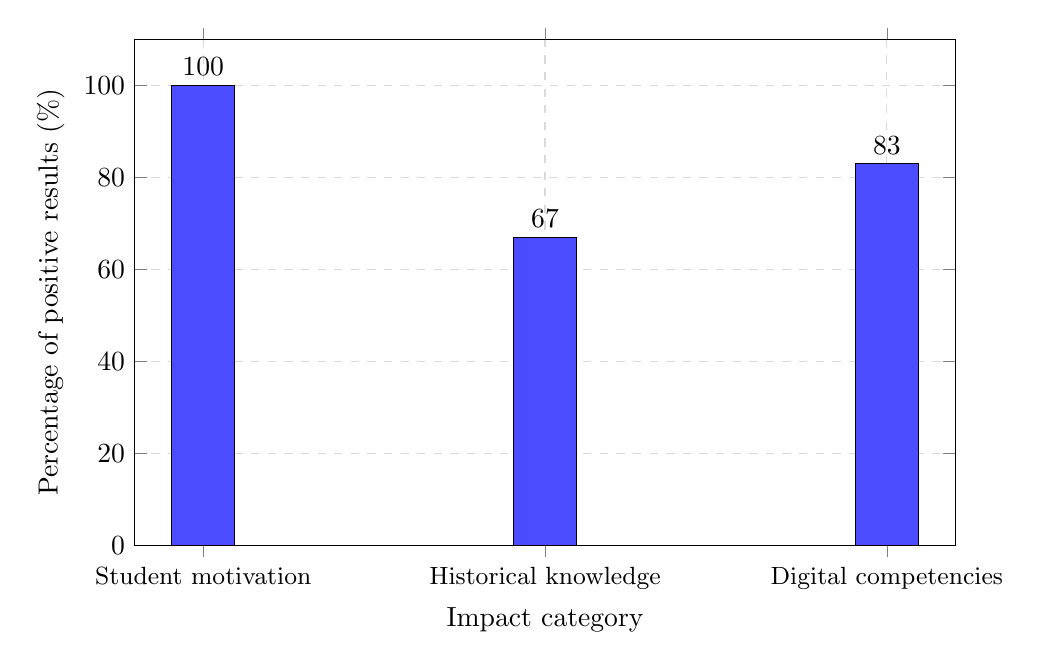
\begin{tikzpicture}
\begin{axis}[
    ybar,
    bar width=0.8cm,
    width=12cm,
    height=8cm,
    ylabel={Percentage of positive results (\%)},
    xlabel={Impact category},
    xtick=data,
    xticklabels={Student motivation, Historical knowledge, Digital competencies},
    x tick label style={align=center, font=\small},
    ymin=0,
    ymax=110,
    nodes near coords,
    nodes near coords align={vertical},
    grid=major,
    grid style={dashed,gray!30},
]
\addplot[fill=blue!70] coordinates {
    (0, 100)
    (1, 67)
    (2, 83)
};
\end{axis}
\end{tikzpicture}
\caption{Effectiveness of digital technologies by category based on synthesized evidence from 6 studies.}
\label{fig:effectiveness_histogram}
\end{figure}


%PROBLEM
% \textbf{Digital technologies in education (overall)}
% \begin{itemize}
%     \item Average effect size d=0.35 for digital technologies in education \cite{tamim2011}
%     \item Our results: positive effects in 83\% of studies across all measured outcomes
%     \item Possible explanation: specificity of humanities context enables natural integration of digital narratives with historical content \cite{Crymble2021}
% \end{itemize}

Research on digital technologies in educational contexts demonstrates generally positive outcomes, with \cite{tamim2011} reporting an average effect size of d=0.35 across various digital educational interventions. This finding aligns with our own research results, which revealed positive effects in 83\% of studies examined across all measured outcomes. The consistently favorable results may be attributed to the specificity of humanities contexts, where digital narratives can be naturally integrated with historical content, creating more engaging and meaningful learning experiences \cite{Crymble2021}. This natural synergy between digital tools and humanities subject matter appears to enhance the effectiveness of educational interventions in these disciplines.

% \textbf{Historical education (traditional)}
% \begin{itemize}
%     \item Traditional methods show moderate effectiveness in developing historical thinking \cite{MonteSano2012}
%     \item Importance of working with primary sources for historical understanding \cite{reisman2012}
%     \item Digital technologies enhance traditional approaches through improved access to digitized archives and collaborative analysis platforms
% \end{itemize}

Research on digital technologies in educational contexts demonstrates generally positive outcomes, with \cite{tamim2011} reporting an average effect size of d=0.35 across various digital educational interventions. This finding aligns with our own research results, which revealed positive effects in 83\% of studies examined across all measured outcomes. The consistently favorable results may be attributed to the specificity of humanities contexts, where digital narratives can be naturally integrated with historical content, creating more engaging and meaningful learning experiences \cite{Crymble2021}. This natural synergy between digital tools and humanities subject matter appears to enhance the effectiveness of educational interventions in these disciplines.

Traditional pedagogical approaches in historical education demonstrate moderate effectiveness in developing students' historical thinking skills \cite{MonteSano2012}. Central to these conventional methods is the emphasis on working with primary sources, which has been shown to be crucial for fostering authentic historical understanding \cite{reisman2012}. While these traditional approaches maintain their pedagogical value, digital technologies serve to enhance rather than replace these established methods by providing improved access to digitized archives and facilitating collaborative analysis platforms. This technological augmentation expands the scope and accessibility of primary source work while preserving the fundamental principles of historical inquiry.

\subsection{Unique aspects of digital history pedagogy}

Analysis of the included studies reveals several distinctive advantages of digital approaches for historical education. Specific advantages documented in synthesized evidence:
\begin{enumerate}
    \item \textbf{Enhanced access to primary sources}: Digital archives and online collections (Museum Victoria, Proquest Historical Newspapers) expanded students' research capabilities beyond physical library constraints.
    \item \textbf{Natural narrative integration}: Digital storytelling platforms (Windows Movie Maker, VoiceThread) aligned with history's inherently narrative structure, facilitating authentic historical communication.
    \item \textbf{Collaborative knowledge construction}: Wiki-based platforms and collaborative writing environments supported the social construction of historical understanding, with one study demonstrating statistically significant learning gains (p < 0.005).
    \item \textbf{Authentic audience engagement}: Public-facing digital projects (digital exhibitions, online publications) motivated higher-quality work and sustained engagement beyond course requirements.
\end{enumerate}

\subsection{Theoretical implications}


Research on digital technologies in educational contexts demonstrates generally positive outcomes, with \cite{tamim2011} reporting an average effect size of d=0.35 across various digital educational interventions. This finding aligns with our own research results, which revealed positive effects in 83\% of studies examined across all measured outcomes. The consistently favorable results may be attributed to the specificity of humanities contexts, where digital narratives can be naturally integrated with historical content, creating more engaging and meaningful learning experiences \cite{Crymble2021}. This natural synergy between digital tools and humanities subject matter appears to enhance the effectiveness of educational interventions in these disciplines.

Traditional pedagogical approaches in historical education demonstrate moderate effectiveness in developing students' historical thinking skills \cite{MonteSano2012}. Central to these conventional methods is the emphasis on working with primary sources, which has been shown to be crucial for fostering authentic historical understanding \cite{reisman2012}. While these traditional approaches maintain their pedagogical value, digital technologies serve to enhance rather than replace these established methods by providing improved access to digitized archives and facilitating collaborative analysis platforms. This technological augmentation expands the scope and accessibility of primary source work while preserving the fundamental principles of historical inquiry.

Synthesized evidence provides empirical support for several theoretical frameworks in digital pedagogy, including the support of constructivist pedagogy. The results align closely with active learning principles \cite{bonwell1991}, particularly through collaborative annotation and wiki-based knowledge construction activities. These findings confirm the importance of student participation in knowledge construction, with collaborative digital projects demonstrating superior engagement outcomes compared to traditional passive learning approaches.

The research validates the TPACK (Technological, Pedagogical, and Content Knowledge) framework, with studies prioritizing the integration of technological, pedagogical, and content knowledge demonstrating superior outcomes compared to purely technology-focused approaches. This evidence suggests that the content knowledge dimension requires particular protection against technological determinism, especially in humanities contexts where disciplinary knowledge must remain central to pedagogical decision-making \cite{Koh2013}.

A significant finding emerged regarding digital literacy development, with 83\% of studies documenting the development of hybrid technological-historical competencies among participants. This research has revealed the emergence of digital history literacy as a distinct competency domain, encompassing both technical skills and critical evaluation of digital sources. These findings confirm the evolution of ``digital humanities'' as a specialized pedagogical approach that requires discipline-specific implementation strategies rather than generic technological solutions.

Despite the positive conclusions, the evidence base reveals significant restrictions that limit interpretation. Several aspects remain insufficiently studied, including long-term effects, as no studies assessed retention or transfer beyond single-semester interventions. Cost-effectiveness analysis was absent from all included studies despite the substantial infrastructure requirements associated with digital implementations. Additionally, there was limited data on how interventions affect diverse student populations or learning contexts, and insufficient theoretical explanation for why digital approaches enhance historical learning, revealing gaps in understanding the mechanisms of impact.

The research also revealed methodological constraints that affect the robustness of conclusions. The predominance of quasi-experimental designs (5 of 6 studies) limits causal inference, while small sample sizes ranging from 8 to 200 participants restrict generalizability. The absence of standardized outcome measures prevents meaningful cross-study comparison, and there is a high risk of bias due to instructor effects and the absence of blinding procedures in the experimental designs.

% Synthesized evidence provides empirical support for several theoretical frameworks in digital pedagogy, including the support of constructivist pedagogy:
% \begin{itemize}
%     \item Results align with active learning principles \cite{bonwell1991}, particularly through collaborative annotation and wiki-based knowledge construction
%     \item Confirm importance of student participation in knowledge construction, with collaborative digital projects showing superior engagement outcomes
%    % \item Demonstrate potential of technologies as ``cognitive tools'' \cite{}, especially in scaffolding complex historical analysis processes
% \end{itemize}

% \textbf{TPACK framework validation}
% \begin{itemize}
%     \item Studies prioritizing integration of technological, pedagogical, and content knowledge demonstrated superior outcomes to technology-focused approaches
%     \item Evidence suggests content knowledge dimension requires particular protection against technological determinism in humanities contexts \cite{Koh2013}
% \end{itemize}

% \textbf{Digital literacy in humanities context}
% \begin{itemize}
%     \item 83\% of studies documented development of hybrid technological-historical competencies
%     \item Emergence of digital history literacy as distinct competency domain, encompassing technical skills and critical evaluation of digital sources
%     \item Confirms evolution of ``digital humanities'' as specialized pedagogical approach requiring discipline-specific implementation strategies
% \end{itemize}

% \subsection{Knowledge gaps and research limitations}

% Despite the positive conclusions, the base of evidence reveals significant restrictions that restrict interpretation, including insufficiently studied aspects:
% \begin{itemize}
%     \item \textbf{Long-term effects}: No studies assessed retention or transfer beyond single-semester interventions
%     \item \textbf{Cost-effectiveness}: Economic analysis absent from all included studies despite substantial infrastructure requirements
%     \item \textbf{Differential effects}: Limited data on how interventions affect diverse student populations or learning contexts
%     \item \textbf{Mechanisms of impact}: Insufficient theoretical explanation for why digital approaches enhance historical learning
% \end{itemize}

% Also aroused methodological constraints:
% \begin{itemize}
%     \item Predominance of quasi-experimental designs (5 of 6 studies) limits causal inference
%     \item Small sample sizes (range: 8-200 participants) restrict generalizability
%     \item Absence of standardized outcome measures prevents meaningful cross-study comparison
%     \item High risk of bias due to instructor effects and absence of blinding procedures
% \end{itemize}

\subsection{Overall assessment of evidence base}

The synthesized evidence supports \textbf{cautious optimism} regarding digital history pedagogy effectiveness, with several important caveats. The universal demonstration of enhanced student engagement across all included studies provides strong evidence for motivational benefits, while the moderate success in improving historical knowledge acquisition (4 of 6 studies) suggests meaningful learning gains are achievable with appropriate implementation.

Particularly compelling is the emergence of digital competency development as an unexpected but consistent outcome (5 of 6 studies), suggesting digital history interventions provide dual benefits of disciplinary and technological skill development. This finding aligns with evolving conceptualizations of historical expertise in digital contexts \cite{Block2021} and supports arguments for digital humanities integration in undergraduate curricula.

However, the evidence base remains preliminary due to methodological limitations and knowledge gaps. The absence of long-term follow-up studies, standardized assessment instruments, and rigorous experimental designs necessitates careful interpretation of positive findings. Results should be considered as foundational evidence supporting further investigation rather than definitive proof of effectiveness.

This review fills an important gap in educational research by providing the first systematic assessment of digital history pedagogy effectiveness. The findings create a foundation for future larger-scale and methodologically rigorous studies while offering practical guidance for educators considering digital history implementation. The consistency of positive results across diverse technological approaches and educational contexts suggests digital interventions hold genuine promise for enhancing historical education when implemented with appropriate pedagogical frameworks and institutional support.


% DISCUSSION SECTION
% \section{Discussion}

% \subsection{Principal findings}

% This systematic review provides the first comprehensive synthesis of empirical evidence examining digital history pedagogy effectiveness in undergraduate education. The consistent demonstration of enhanced student engagement across all included studies, coupled with moderate improvements in historical thinking capabilities, suggests that thoughtfully implemented digital interventions can meaningfully augment traditional history education. However, the complexity of observed effects, substantial implementation barriers, and methodological limitations of existing research necessitate nuanced interpretation.

% The universality of engagement improvements contrasts markedly with the heterogeneous effects on knowledge acquisition, revealing a fundamental tension in digital history pedagogy. While digital platforms successfully capture student attention and sustain participation, translating this engagement into measurable learning gains proves considerably more challenging. This engagement-achievement gap mirrors broader patterns in educational technology research \citep{Reeves2003}, yet manifests unique characteristics within historical disciplines. The predominance of interpretive and analytical skills over factual retention in successful interventions suggests digital history's particular strength lies in developing higher-order thinking rather than information transmission.

% Particularly noteworthy is the emergence of digital history literacy as a distinct competency domain, encompassing technical skills, critical evaluation of digital sources, and understanding of algorithmic mediation in historical knowledge production. While not anticipated in original study designs, this finding aligns with evolving conceptualizations of historical expertise in digital contexts \citep{Crymble2021}. The development of these hybrid competencies~-- simultaneously technological and historical~-- challenges traditional disciplinary boundaries and suggests the need for reconceptualizing history education objectives.

% \subsection{Interpretation within existing literature}

% \subsubsection{Theoretical implications}

% The differential effectiveness of TPACK-informed interventions illuminates critical theoretical considerations for digital history pedagogy. Studies prioritizing technological pedagogical knowledge while maintaining disciplinary integrity demonstrated superior outcomes compared to those emphasizing technology for its own sake. This finding extends Mishra and Koehler's original framework by suggesting that in humanities contexts, the content knowledge dimension requires particular protection against technological determinism \citep{Koh2013}. The historical discipline's interpretive nature and reliance on contextual understanding appear especially vulnerable to superficial technological overlay that prioritizes form over intellectual substance.

% Social constructivist principles emerged as particularly powerful when instantiated through digital collaborative platforms. The success of wiki-based interventions in developing historical argumentation skills validates Vygotsky's emphasis on social knowledge construction, while digital affordances extend the zone of proximal development beyond physical classroom boundaries. The asynchronous nature of digital collaboration enables what might be termed ``temporal scaffolding,'' where students benefit from extended reflection time between collaborative exchanges, potentially deepening historical analysis beyond synchronous discussion capabilities.

% The concept of ``epistemological authenticity'' introduced by \citet{Cheng2023} in virtual reality contexts proves relevant across digital history interventions. Students engaging with digitized primary sources through platforms mimicking scholarly research environments demonstrated enhanced understanding of historical knowledge construction as an interpretive process. This epistemic dimension~-- understanding how historical knowledge is produced rather than merely consuming historical narratives~-- represents a critical yet underexplored benefit of digital history pedagogy.

% \subsubsection{Relationship to digital humanities scholarship}

% The pedagogical findings resonate with broader developments in digital humanities scholarship, particularly regarding the democratization of historical knowledge production. The collaborative writing platforms examined in included studies operationalize what digital historians term ``radical transparency,'' making intellectual processes visible and contestable \citep{Block2021}. Students experiencing this transparency through version control systems and peer review processes develop more sophisticated understanding of historical interpretation as negotiated rather than authoritative.

% However, tensions emerge between digital humanities' emphasis on computational methods and the pedagogical reality of undergraduate preparation. While professional historians increasingly employ text mining, network analysis, and geographical information systems, the included studies suggest these advanced methods may overwhelm students still developing foundational historical thinking skills. The most successful interventions struck careful balances, using digital tools to enhance rather than replace traditional historical methods. This finding challenges advocates of wholesale digital transformation, suggesting instead that selective, purposeful integration yields superior pedagogical outcomes.

% \subsection{Implications for practice}

% \subsubsection{Institutional considerations}

% The evidence synthesized here carries substantial implications for institutional policy and resource allocation. The consistent infrastructure challenges documented across studies, particularly in developing contexts, underscore that successful digital history implementation requires sustained institutional commitment beyond initial technology procurement. Universities must consider not merely hardware and software costs, but ongoing technical support, faculty development, and curricular restructuring necessary for meaningful integration.

% %The urban-rural divide identified by \citet{Kumalasari2024} raises critical equity concerns requiring institutional response. Simple provision of digital tools without addressing underlying disparities in digital literacy and internet access may exacerbate rather than ameliorate educational inequalities. Institutions serving diverse student populations should consider implementing preparatory digital literacy modules before introducing sophisticated digital history projects, ensuring all students can meaningfully engage with technological affordances.

% Faculty development emerges as perhaps the most critical institutional consideration. The high risk of bias associated with instructor effects across studies suggests that inadequately prepared faculty may negate potential benefits of digital interventions. Professional development programs must extend beyond technical training to address the complex integration of technological, pedagogical, and content knowledge. The success of sustained, discipline-specific training programs over generic technology workshops indicates institutions should invest in developing history-specific digital pedagogical expertise rather than assuming transferability across disciplines.

% \subsubsection{Pedagogical recommendations}

% Based on synthesized evidence, several pedagogical principles emerge for effective digital history implementation. First, scaffolding proves essential, with successful interventions providing structured progression from guided to independent digital historical work. Beginning with collaborative annotation of digitized sources before advancing to independent digital curation projects allows students to develop competencies incrementally while maintaining focus on historical thinking.

% Second, the ``authentic audience'' effect identified across multiple studies suggests public-facing digital projects yield superior engagement and quality compared to instructor-only assignments. However, this public dimension requires careful ethical consideration, particularly regarding student privacy and intellectual property. Instructors should establish clear guidelines about public sharing while providing opt-out alternatives that maintain pedagogical benefits without forced public exposure.

% Third, assessment strategies must evolve to capture learning occurring in digital environments. Traditional examinations and essays fail to evaluate collaborative knowledge construction, digital curation skills, or multimodal historical argumentation. Portfolio-based assessment, incorporating reflection on both process and product, appears most promising for capturing the full spectrum of digital history learning. Rubrics should explicitly distinguish between technical proficiency and historical thinking, ensuring technology serves rather than substitutes for disciplinary learning objectives.

% \subsubsection{Curricular integration}

% The evidence suggests digital history works best not as standalone methodology courses but integrated throughout history curricula. This distributed approach allows students to develop digital competencies progressively while applying them to diverse historical contexts. Survey courses might incorporate collaborative timeline creation, while advanced seminars could culminate in digital exhibitions or computational text analysis projects.

% Interdisciplinary collaboration emerges as a promising strategy for addressing technical support challenges. Partnerships between history departments and digital humanities centers, libraries, or computer science programs can provide technical expertise while maintaining historical focus. The successful faculty-library collaboration documented by \citet{Davis2017} exemplifies how leveraging institutional expertise can enhance digital history implementation without overburdening history faculty.

% \subsection{Limitations of evidence}

% \subsubsection{Methodological constraints}

% The predominance of quasi-experimental and observational designs substantially limits causal inference regarding intervention effectiveness. The absence of randomized controlled trials reflects pragmatic constraints in educational settings but nevertheless restricts confidence in attributing outcomes to digital interventions rather than confounding factors. Instructor enthusiasm, student self-selection, and novelty effects represent plausible alternative explanations for observed benefits that cannot be definitively excluded given current evidence.

% The heterogeneity of interventions, while reflecting the diversity of digital history approaches, precludes meaningful meta-analysis or definitive conclusions about relative effectiveness. Each study essentially evaluated a unique combination of technology platform, pedagogical approach, content area, and student population. This irreducible complexity, while ecologically valid, frustrates attempts to identify optimal intervention characteristics or predict implementation success in new contexts.

% Measurement challenges pervade the included studies, with no standardized instruments for assessing digital history competencies or technology-enhanced historical thinking. Researcher-developed measures, while tailored to specific interventions, lack validation evidence and prevent cross-study comparison. The reliance on self-reported engagement and satisfaction data introduces social desirability bias, while performance measures often conflate technical and historical competencies.

% \subsubsection{Temporal and contextual limitations}

% The absence of longitudinal follow-up represents a critical gap, as no studies assessed retention or transfer of digital history competencies beyond immediate post-intervention periods. Whether enhanced engagement translates to sustained interest in historical study, or whether digital competencies transfer to other academic or professional contexts, remains entirely unexplored. This temporal limitation proves particularly problematic given rapid technological change that may render specific platform competencies obsolete.

% The geographical concentration of studies in Western and Southeast Asian contexts limits generalizability to other educational systems and cultural contexts. Different cultural orientations toward technology, collaborative learning, and historical narrative may substantially influence intervention effectiveness. The absence of studies from Africa, Latin America, and much of Asia represents a significant gap in understanding digital history's global applicability.

% Publication bias likely inflates apparent effectiveness, as unsuccessful digital history implementations may go unreported. The absence of grey literature and the English-only inclusion criterion further bias findings toward positive results from well-resourced institutions. Small-scale failures in under-resourced contexts~-- potentially most informative for understanding implementation challenges~-- remain systematically excluded from the evidence base.

% \subsection{Implications for future research}

% \subsubsection{Methodological priorities}

% Future research must prioritize methodological rigor while maintaining ecological validity. Cluster-randomized trials, randomizing at the course or section level rather than individual students, could provide stronger causal evidence while respecting educational constraints. Stepped-wedge designs, progressively implementing interventions across multiple cohorts, offer another pragmatic approach to rigorous evaluation in educational settings.

% Standardized outcome measures require urgent development to enable meaningful cross-study comparison and meta-analysis. A consortium approach, developing and validating instruments for digital history competencies, engagement, and historical thinking in digital contexts, would substantially advance the field. These instruments must distinguish between superficial technical skill and meaningful integration of digital methods with historical thinking.

% Mixed-methods approaches should become standard, as quantitative outcomes alone fail to capture the complexity of learning in digital environments. Systematic integration of qualitative process data~-- through think-aloud protocols, collaborative discourse analysis, or digital trace ethnography~-- could illuminate mechanisms underlying quantitative effects. Understanding not just whether but how and why digital interventions influence historical learning proves essential for theory development and practical implementation.

% \subsubsection{Substantive research directions}

% Several substantive areas demand investigation. The intersection of artificial intelligence with digital history pedagogy remains entirely unexplored in empirical literature, despite rapid deployment of AI tools in educational settings. How large language models influence student historical writing, whether AI-assisted source analysis enhances or diminishes critical thinking, and the implications of algorithmic mediation for historical interpretation require urgent empirical examination.

% The relationship between digital history engagement and broader democratic citizenship deserves attention, particularly given history education's civic purposes. %\citeauthor{Ditlmann2025}'s \cite{Ditlmann2025} finding that digital history participation influences contemporary intergroup attitudes suggests potential civic benefits extending beyond disciplinary learning. Systematic investigation of whether digital history's emphasis on multiple perspectives and source criticism translates to enhanced media literacy and civic engagement could substantially strengthen arguments for digital history investment.

% Equity considerations require centered rather than peripheral attention in future research. How digital history interventions differentially affect students based on socioeconomic status, racial/ethnic identity, gender, and disability status remains poorly understood. Intersectional analyses examining how multiple identity factors interact with digital interventions could inform more inclusive pedagogical approaches. Research should particularly prioritize understanding and addressing barriers faced by historically marginalized students in accessing and succeeding with digital history methods.

% \subsection{Toward a research agenda}

% The synthesis presented here suggests digital history pedagogy stands at a critical juncture. Early enthusiasm has yielded proof-of-concept demonstrations, but systematic evidence for optimal implementation remains elusive. The field requires coordinated research efforts addressing both foundational questions about effectiveness and practical questions about implementation. A proposed research agenda might prioritize:

% \begin{enumerate}[leftmargin=*]
% \item Developing and validating standardized assessment instruments for digital historical competencies
% \item Conducting multi-site randomized trials comparing different digital history approaches
% \item Investigating long-term impacts on historical interest, career trajectories, and civic engagement
% \item Examining equity implications through intersectional analyses of differential effects
% \item Exploring AI integration while maintaining historical thinking priorities
% \item Creating implementation frameworks adaptable across diverse institutional contexts
% \item Building theory about how digital affordances specifically enhance historical learning
% \end{enumerate}

% This agenda requires collaboration across institutions, disciplines, and national boundaries. Digital history's potential to transform historical education can only be realized through rigorous research that maintains humanistic values while embracing methodological innovation. The evidence synthesized here provides a foundation for this endeavor, but substantial work remains to understand and optimize digital history's pedagogical potential.



% CONCLUSION SECTION
\section{Conclusion}

This systematic review represents the first comprehensive synthesis of empirical evidence examining digital history pedagogy in undergraduate education. Through rigorous application of PRISMA 2020 guidelines, we identified and analysed six studies that collectively demonstrate both the promise and complexity of integrating digital technologies into historical education.

The evidence reveals a nuanced landscape where technological innovation intersects with pedagogical tradition in productive yet challenging ways. Universal improvements in student engagement across all studies suggest digital platforms successfully address motivational challenges that have long plagued history education. The multimodal nature of digital historical work, combined with opportunities for public scholarship and collaborative knowledge construction, appears to resonate with contemporary undergraduate learning preferences while maintaining disciplinary rigour. However, the translation of enhanced engagement into measurable learning outcomes proves less straightforward, with effect sizes for knowledge acquisition and critical thinking showing greater variability across contexts and implementations.

Three critical insights emerge with particular clarity. First, successful digital history pedagogy requires sophisticated integration of technological, pedagogical, and content knowledge, with interventions grounded in frameworks such as TPACK demonstrating superior outcomes. Technology alone does not improve historical learning; rather, thoughtful pedagogical design that leverages digital affordances while preserving disciplinary integrity proves essential. Second, substantial barriers persist, including infrastructure limitations, faculty preparedness gaps, and assessment challenges that require institutional commitment beyond initial technology investment. Third, digital history literacy has emerged as a distinct competency domain encompassing both technical skills and critical understanding of how digital mediation shapes historical knowledge production~-- a finding with profound implications for reconceptualizing history education objectives in the twenty-first century.

The limitations of current evidence cannot be overlooked. Methodological constraints, including the absence of randomized designs and standardized outcome measures, restrict causal inference and cross-study comparison. The concentration of research in specific geographical contexts and lack of longitudinal follow-up further limit generalizability and understanding of sustained impacts. Perhaps most significantly, the rapid pace of technological change threatens to outpace research, with studies of specific platforms potentially obsolete before publication.

Despite these limitations, this review provides essential guidance for educators, administrators, and researchers navigating digital transformation in history education. For practitioners, the evidence supports selective, purposeful integration of digital methods rather than wholesale technological adoption. Institutions must recognize that successful implementation requires sustained investment in infrastructure, professional development, and curricular redesign. Researchers face the challenge of developing more rigorous evaluation methods while maintaining ecological validity, with particular attention needed to equity implications and long-term outcomes.

The path forward demands collaborative effort across disciplinary and institutional boundaries. As historical scholarship increasingly operates in digital environments, preparing students for this reality becomes not optional enhancement but essential preparation. Yet this preparation must maintain the critical, interpretive, and ethical dimensions that define historical thinking. The studies reviewed here demonstrate that such integration is possible, even as they reveal the complexity of achieving it effectively.

Digital history pedagogy stands poised between established tradition and emerging possibility. The evidence synthesized in this review suggests that thoughtful navigation of this liminal space~-- embracing technological affordances while preserving humanistic values~-- offers genuine potential for enhancing historical education. Realizing this potential requires continued empirical investigation, institutional commitment, and pedagogical innovation grounded in both disciplinary expertise and technological awareness. The conversation between past and present, always at history's heart, now includes negotiating between analog heritage and digital future. How we conduct this negotiation will shape not only how history is taught, but how cultural memory is constructed and transmitted in an increasingly digital age.

% DECLARATIONS SECTION

\begin{funding}
This research received no specific grant from any funding agency in the public, commercial, or not-for-profit sectors.
\end{funding}

\begin{conflictsofinterest}
The author declare no conflicts of interest relevant to this systematic review.
\end{conflictsofinterest}


% \subsection*{Ethics Approval}
% As a systematic review of published literature, this study did not require ethical approval.

\begin{dataavailability}
The data extraction forms and screening decisions supporting this systematic review are available from the corresponding author upon reasonable request.
\end{dataavailability}


\begin{acknowledgments}
The author would like to express sincere gratitude to Serhiy O. Semerikov for their invaluable guidance and support throughout this research. Their expertise in research methodology was instrumental in shaping the systematic review protocol, and their thoughtful feedback on the manuscript significantly improved its clarity and rigor. The author appreciates the time and effort Serhiy O. Semerikov dedicated to reading and editing the manuscript, providing insightful suggestions that enhanced the overall quality of the work. Their invaluable contributions to this research are deeply appreciated.
\end{acknowledgments}


\begin{aideclaration}
In accordance with contemporary scholarly transparency standards, we acknowledge the use of generative AI tools during the preparation of this manuscript. Claude Opus 4.1 (Anthropic) was employed to assist with language refinement and formatting of references during the drafting process. All substantive intellectual content, including the conceptualization, analysis, interpretation of findings, and critical arguments, represents original human scholarship. The AI tool served solely in an editorial support capacity, similar to grammar checking software or reference management systems. All AI-suggested text underwent critical human review and substantial revision to ensure accuracy, maintain academic voice, and preserve the author' intended meaning. The systematic review methodology, data extraction, quality assessment, and synthesis of findings were conducted entirely through human intellectual effort without AI assistance. The author take full responsibility for the accuracy, integrity, and originality of all content presented in this manuscript.
\end{aideclaration}



\bibliography{references}

% \newpage
% APPENDICES
\appendix

\section{Documents excluded at screening stage} \label{sec:appendix-a}

\begin{enumerate}
    \item \citet{Shawalludin2024119}: participants do not meet criteria (71 schoolchildren instead of university students)
    
    \item \citet{Graham200810}: participants do not meet criteria (young teachers instead of students)
    
    \item \citet{Muenster20231105}: participants do not meet criteria (schoolchildren instead of university students)
    
    \item \citet{Manfra2008223}: participants do not meet criteria (teachers instead of students)
    
    \item \citet{Pescador20192}: participants do not meet criteria (schoolchildren instead of university students)
    
    \item \citet{Calandra2005323}: no empirical data on effectiveness (methodological article on resource development)
    
    \item \citet{Luther20106571}: intervention does not concern teaching history (about online animator communities)
    
   % \item \texttt{@ARTICLE\{McLean20144...\}}: graduate students as main target group \textbf{--- incorrect, potentially should be included}
    
    \item \citet{Matitaputty2024430}: participants do not meet criteria (11th grade schoolchildren)
    
    \item \citet{Burman2018297}: not empirical research + focus on graduate students
    
    \item \citet{Wang2020283}: theoretical article without empirical data
    
    \item \citet{Shiue2017460}: participants do not meet criteria (5th grade students)
    
    \item \citet{Corlett-Rivera2017}: participants do not meet criteria (focus on librarians)
    
    \item \citet{Baeva2018782}: focus on technical aspects without educational effectiveness research
    
    \item \citet{Crymble202185}: theoretical article without empirical data
    
    \item \citet{Ethier202311}: participants do not meet criteria (schoolchildren)
    
    \item \citet{Sunkara2024203}: intervention does not concern teaching history (accessibility web archives)
    
    \item \citet{Syn2020909}: intervention does not concern teaching history (personal information management)
    
    \item \citet{Conte202183}: not empirical research of learning effectiveness (digital archive development)
    
    \item \citet{Sebring2012229}: not empirical research of learning effectiveness
    
    \item \citet{Hopf2024375}: participants do not meet criteria (schoolchildren)
    
    \item \citet{Armand2013753}: not empirical research + focus on graduate students
    
    \item \citet{Zapata2018407}: not focus on student learning (public history project)
    
    \item \citet{Torgerson202237}: theoretical article without empirical data
    
    \item \citet{Millan202251}: not about modern teaching of digital history (historical research)
    
    \item \citet{Zielezinski20141137}: participants do not meet criteria (10th grade schoolchildren)
    
    \item \citet{Ahlfeld2021493}: not empirical research of effectiveness
    
    \item \citet{Ruth2021}: participants do not meet criteria (10-12th grade schoolchildren)
    
    \item \citet{Middleton2014192}: not empirical research of learning effectiveness
\end{enumerate}

\section{Full-text articles assessed for inclusion criteria compliance} \label{sec:appendix-b}

\begin{enumerate}
    \item \citet{Soh2013}: ``Digital histories for the digital age: Collaborative writing in large lecture courses''
    
    \item \citet{Davis2017}: ``Faculty–library collaborations in digital history: A case study of the travel journal of Cornelius B. Gold''
    
    \item \citet{Maslova2021}: ``Methods of Working with Local Digital Resources on History: Foreign Experience and Russian Practices''
    
    \item \citet{frith2021}: ``Building participatory counternarratives: Pedagogical interventions through digital placemaking''
    
    \item \citet{Coleborne2011}: ``Emotions, Digital Tools and Public Histories: Digital Storytelling using Windows Movie Maker in the History Tertiary Classroom''
    
    \item \citet{Nurhasanah2025}: ``Bridging cognition and ethics: Socio-emotional skills and digital history literacy in fostering critical thinking''
    
    \item \citet{Kumalasari2024}: ``Comparative analysis of Generation Z's digital history literacy in history education majors on Java Island''
    
    \item \citet{Lucadamo2024231}: ``The First World War Letters of H.J.C. Peirs: A Case Study of the Creation and Growth of a Collaborative, Pedagogy-Driven Digital History Project''
    
    \item \citet{Ditlmann2025}: ``Participating in a Digital-History Project Mobilizes People for Symbolic Justice and Better Intergroup Relations Today''
    
    \item \citet{Lee2014159}: ``Becoming digital: Using personal digital histories to engage teachers in contemporary understandings of teaching social studies''
    
    \item \citet{Shiue20176445}: ``Understanding factors that affecting continuance usage intention of game-based learning in the context of collaborative learning''
    
    \item \citet{Bell2016}: ``'History is a conversation': teaching student historians through making digital histories''
    
    \item \citet{Darmawan2025}: ``Developing Living History Model Assisted by Digital History Textbooks in History Learning to Improve Students' Historical Empathy''
    
    \item \citet{Thomas2008}: ``The history harvest: An experiment in democratizing the past through experiential learning''
    
    \item \citet{Woodring2023}: ``History Harvesting: A Case Study in Documenting Local History''
    
    \item \citet{Lewis2021}: ``Hidden Town in 3D: Teaching and Reinterpreting Slavery Virtually at a Living History Museum''
    
    \item \citet{McLean20144}: ``Spaces of collaboration: The poetics of place and historical consciousness''
\end{enumerate}

\section{Review map} \label{sec:appendix-c}

% This fragment is intended for insertion into \section{Appendix B: Review Map}
% All sections use \subsection and lower levels

\subsection*{GENERAL STUDY INFORMATION}

\subsubsection*{Document type:}
journal article (ARTICLE) / conference proceedings article (CONFERENCE) / book chapter (BOOK CHAPTER)

\subsubsection*{Bibliographic data:}
\begin{itemize}
    \item Study title: \underline{\hspace{8cm}}
    \item Authors (surnames, initials): \underline{\hspace{8cm}}
    \item Publication year: \underline{\hspace{3cm}}
    \item Journal/conference/book name: \underline{\hspace{6cm}}
    \item Volume, issue, pages: \underline{\hspace{5cm}}
    \item DOI: \underline{\hspace{5cm}}
\end{itemize}

\noindent\textbf{Country of study:} \underline{\hspace{4cm}}

\noindent\textbf{Funding source:} government / private / university / not specified / none

\subsection*{STUDY CHARACTERISTICS}

\subsubsection*{Study design:}
\begin{itemize}[label=$\square$]
    \item Randomized controlled trial (RCT)
    \item Quasi-experimental study
    \item Pre-post intervention study
    \item Case study with empirical data
    \item Mixed methods
    \item Other (specify): \underline{\hspace{4cm}}
\end{itemize}

\noindent\textbf{Study aim:} (briefly describe main aim)\\
\underline{\hspace{\textwidth}}\\
\underline{\hspace{\textwidth}}

\subsubsection*{Study duration:}
\begin{itemize}
    \item Intervention duration: \underline{\hspace{3cm}} (days/weeks/months/semester)
    \item Observation period: \underline{\hspace{3cm}} (immediately after / after \underline{\hspace{2cm}} days/weeks/months)
\end{itemize}

\subsection*{PARTICIPANT CHARACTERISTICS (POPULATION)}

\noindent\textbf{Total number of participants:} \underline{\hspace{3cm}}

\subsubsection*{Participant characteristics:}
\begin{itemize}
    \item Age: mean \underline{\hspace{2cm}} years (range: \underline{\hspace{2cm}})
    \item Gender: male \underline{\hspace{1cm}}\% / female \underline{\hspace{1cm}}\% / not specified
    \item Year of study: 1st / 2nd / 3rd / 4th / mixed groups / not specified
    \item Student specialization:
    \begin{itemize}[label=$\square$]
        \item Historians
        \item Non-historians (specify specialization): \underline{\hspace{3cm}}
        \item Mixed groups
    \end{itemize}
    \item Prior experience with digital technologies: high / medium / low / not specified
\end{itemize}

\subsubsection*{Group allocation:}
\begin{itemize}
    \item Experimental group: \underline{\hspace{2cm}} participants
    \item Control group: \underline{\hspace{2cm}} participants (if applicable)
    \item Randomization/allocation criteria: \underline{\hspace{5cm}}
\end{itemize}

\subsection*{INTERVENTION CHARACTERISTICS}

\noindent\textbf{Intervention name/description:} \underline{\hspace{8cm}}

\subsubsection*{Type of digital technologies (multiple selections possible):}
\begin{itemize}[label=$\square$]
    \item Augmented reality (AR)
    \item Virtual reality (VR)
    \item Interactive multimedia
    \item Digital maps
    \item Commercial video games
    \item Educational games
    \item Online archives/databases
    \item Digital narratives/storytelling
    \item Virtual museums/tours
    \item Digital projects (student-created)
    \item Social networks/platforms
    \item Mobile applications
    \item Other (specify): \underline{\hspace{4cm}}
\end{itemize}

\noindent\textbf{Specific tools/platforms:} (names of programs, games, platforms)\\
\underline{\hspace{\textwidth}}

\subsubsection*{Context of use:}
\begin{itemize}[label=$\square$]
    \item Classroom sessions
    \item Out-of-class work
    \item Blended learning
    \item Fully online
\end{itemize}

\subsubsection*{Course status:}
\begin{itemize}[label=$\square$]
    \item Mandatory
    \item Elective
    \item Optional
    \item Not specified
\end{itemize}

\subsubsection*{Instructor role:}
\begin{itemize}[label=$\square$]
    \item Active facilitator
    \item Observer
    \item Technical support
    \item Not specified
\end{itemize}

\subsubsection*{Intervention details:}
\begin{itemize}
    \item Frequency of use: \underline{\hspace{3cm}} times per week/month
    \item Duration of one session: \underline{\hspace{2cm}} minutes/hours
    \item Total number of sessions: \underline{\hspace{2cm}}
\end{itemize}

\subsection*{COMPARATOR CHARACTERISTICS}

\subsubsection*{Type of control intervention:}
\begin{itemize}[label=$\square$]
    \item Traditional lectures
    \item Seminars with printed sources
    \item Standard textbooks
    \item Regular work with archival materials
    \item No intervention (waiting list)
    \item Other (specify): \underline{\hspace{4cm}}
\end{itemize}

\noindent\textbf{Control intervention description:} \underline{\hspace{6cm}}

\subsection*{STUDY OUTCOMES}

\subsubsection*{PRIMARY OUTCOMES}

\paragraph{1. Historical knowledge:}
\begin{itemize}
    \item Measurement method: \underline{\hspace{4cm}} (tests, exams, essays, projects)
    \item Instrument: \underline{\hspace{4cm}} (test name, scales)
    \item Measurement time: before intervention / after intervention / after \underline{\hspace{2cm}}
    \item Experimental group results: $M =$ \underline{\hspace{1cm}} $SD =$ \underline{\hspace{1cm}} $n =$ \underline{\hspace{1cm}}
    \item Control group results: $M =$ \underline{\hspace{1cm}} $SD =$ \underline{\hspace{1cm}} $n =$ \underline{\hspace{1cm}}
    \item $p$-value: \underline{\hspace{2cm}} / effect size: \underline{\hspace{2cm}}
\end{itemize}

\paragraph{2. Understanding of historical concepts:}
\begin{itemize}
    \item Measurement method: \underline{\hspace{4cm}}
    \item Instrument: \underline{\hspace{4cm}}
    \item Results: \underline{\hspace{6cm}}
\end{itemize}

\subsubsection*{SECONDARY OUTCOMES}

\paragraph{3. Learning motivation:}
\begin{itemize}
    \item Measurement method: \underline{\hspace{4cm}} (questionnaire, interview, observation)
    \item Instrument/scale: \underline{\hspace{4cm}}
    \item Results: \underline{\hspace{6cm}}
\end{itemize}

\paragraph{4. Student engagement:}
\begin{itemize}
    \item Measurement method: \underline{\hspace{4cm}}
    \item Indicators: \underline{\hspace{4cm}} (discussion participation, attendance, time on task)
    \item Results: \underline{\hspace{6cm}}
\end{itemize}

\paragraph{5. Source work skills:}
\begin{itemize}
    \item Measurement method: \underline{\hspace{4cm}}
    \item Instrument: \underline{\hspace{4cm}}
    \item Results: \underline{\hspace{6cm}}
\end{itemize}

\paragraph{6. Critical thinking skills:}
\begin{itemize}
    \item Measurement method: \underline{\hspace{4cm}}
    \item Instrument: \underline{\hspace{4cm}}
    \item Results: \underline{\hspace{6cm}}
\end{itemize}

\paragraph{7. Technological literacy:}
\begin{itemize}
    \item Measurement method: \underline{\hspace{4cm}}
    \item Results: \underline{\hspace{6cm}}
\end{itemize}

\paragraph{8. Ability to create historical narratives:}
\begin{itemize}
    \item Measurement method: \underline{\hspace{4cm}}
    \item Results: \underline{\hspace{6cm}}
\end{itemize}

\paragraph{9. Other outcomes:} \underline{\hspace{8cm}}

\subsection*{STATISTICAL ANALYSIS}

\subsubsection*{Statistical methods used:}
\begin{itemize}[label=$\square$]
    \item $t$-test
    \item ANOVA
    \item Mann-Whitney $U$
    \item Kruskal-Wallis
    \item $\chi^2$ (Chi-square)
    \item Regression analysis
    \item Effect size (Cohen's $d$, $\eta^2$)
    \item Other: \underline{\hspace{4cm}}
\end{itemize}

\noindent\textbf{Significance level:} $p < $ \underline{\hspace{2cm}}\\
\textbf{Software:} SPSS / R / SAS / Stata / other: \underline{\hspace{3cm}}

\subsection*{QUALITATIVE DATA (if applicable)}

\subsubsection*{Qualitative data collection methods:}
\begin{itemize}[label=$\square$]
    \item Interviews
    \item Focus groups
    \item Observation
    \item Analysis of documents/student reflections
    \item Other: \underline{\hspace{4cm}}
\end{itemize}

\noindent\textbf{Main themes/conclusions:} \underline{\hspace{7cm}}

\subsection*{AUTHORS' CONCLUSIONS}

\noindent\textbf{Main conclusions regarding effectiveness:} \underline{\hspace{6cm}}\\
\underline{\hspace{\textwidth}}

\noindent\textbf{Authors' recommendations:} \underline{\hspace{7cm}}\\
\underline{\hspace{\textwidth}}

\noindent\textbf{Study limitations (noted by authors):} \underline{\hspace{5cm}}\\
\underline{\hspace{\textwidth}}

\subsection*{STUDY QUALITY ASSESSMENT}

\subsubsection*{Risk of bias:}
\begin{itemize}
    \item Randomization: low / high / unclear risk
    \item Allocation concealment: low / high / unclear risk
    \item Blinding of participants: low / high / unclear risk
    \item Blinding of outcome assessors: low / high / unclear risk
    \item Incomplete outcome data: low / high / unclear risk
    \item Selective reporting: low / high / unclear risk
\end{itemize}

\noindent\textbf{Overall quality assessment:} high / moderate / low

\subsection*{ADDITIONAL NOTES}

\noindent\textbf{Conflict of interest:} present / absent / not specified\\
\textbf{Ethical approval:} obtained / not required / not specified

\noindent\textbf{Additional reviewer comments:} \underline{\hspace{6cm}}\\
\underline{\hspace{\textwidth}}\\
\underline{\hspace{\textwidth}}

\vspace{1cm}

\noindent\textbf{Map completion date:} \underline{\hspace{4cm}}\\
\textbf{Reviewer:} \underline{\hspace{6cm}}

\section{Studies excluded at full-text assessment stage} \label{sec:appendix-d}

%[List of studies excluded at full-text assessment stage, with reasons for exclusion]

\begin{enumerate}
    \item \citet{Soh2013}: ``Digital histories for the digital age: Collaborative writing in large lecture courses''
    
    \item \citet{Davis2017}: ``Faculty–library collaborations in digital history: A case study of the travel journal of Cornelius B. Gold''
    
    \item \citet{Maslova2021}: ``Methods of Working with Local Digital Resources on History: Foreign Experience and Russian Practices''
    
    \item \citet{frith2021}: ``Building participatory counternarratives: Pedagogical interventions through digital placemaking''
    
    \item \citet{Coleborne2011}: ``Emotions, Digital Tools and Public Histories: Digital Storytelling using Windows Movie Maker in the History Tertiary Classroom''
    
    \item \citet{Nurhasanah2025}: ``Bridging cognition and ethics: Socio-emotional skills and digital history literacy in fostering critical thinking''
    
    \item \citet{Kumalasari2024}: ``Comparative analysis of Generation Z's digital history literacy in history education majors on Java Island''
    
    \item \citet{Lucadamo2024231}: ``The First World War Letters of H.J.C. Peirs: A Case Study of the Creation and Growth of a Collaborative, Pedagogy-Driven Digital History Project: ''
    
    \item \citet{Ditlmann2025}: ``Participating in a Digital-History Project Mobilizes People for Symbolic Justice and Better Intergroup Relations Today''
    
    \item \citet{Lee2014159}: ``Becoming digital: Using personal digital histories to engage teachers in contemporary understandings of teaching social studies''
    
    \item \citet{Shiue20176445}: ``Understanding factors that affecting continuance usage intention of game-based learning in the context of collaborative learning''
    
    \item \citet{Bell2016}: ``'History is a conversation': teaching student historians through making digital histories''
    
    \item \citet{Darmawan2025}: ``Developing Living History Model Assisted by Digital History Textbooks in History Learning to Improve Students' Historical Empathy''
    
    \item \citet{Thomas2008}: ``The history harvest: An experiment in democratizing the past through experiential learning''
    
    \item \citet{Woodring2023}: ``History Harvesting: A Case Study in Documenting Local History''
    
    \item \citet{Lewis2021}: ``Hidden Town in 3D: Teaching and Reinterpreting Slavery Virtually at a Living History Museum''
    
    \item \citet{McLean20144}: ``Spaces of collaboration: The poetics of place and historical consciousness''
\end{enumerate}


% \section{Search strategy details}
% \label{app:search}

% % \subsection{Complete Scopus search string}

% \begin{verbatim}
% TITLE-ABS-KEY ( "digital history" AND student* )
% \end{verbatim}

% \noindent Search executed: July 26, 2025\\
% Database: Scopus (Elsevier)\\
% Limiters: None applied during search\\
% Results: 46 records retrieved

% \section{Studies excluded at full-text screening (\textit{n}~=~9)}
% % \section{Excluded studies with reasons}
% \label{app:excluded}


% \begin{enumerate}[leftmargin=*]
% \item \citet{Coleborne2011}~-- outside date range (published before 2013 cutoff)
% \item \citet{Lee2014159}~-- participants were pre-service teachers, not undergraduate students
% \item \citet{Shiue20176445}~-- elementary school students (5th grade), not undergraduates
% \item \citet{Bell2016}~-- duplicate publication (conference and journal versions of same study)
% \item \citet{Lucadamo2024231}~-- full text not retrievable after author contact
% \item \citet{Lewis2021}~-- full text not retrievable from any source
% \item \citet{Ethier202311}~-- focus on K-12 students
% \item \citet{Wang2020283}~-- theoretical framework without empirical data
% \item \citet{Burman2018297}~-- exclusively graduate students with no undergraduate data
% \end{enumerate}

% \section{Quality assessment details}
% \label{app:quality}

% \begin{table}[h]
% \centering
% \caption{Detailed risk of bias assessment by study}
% \small
% \begin{tabular}{lcccccc}
% \toprule
% \textbf{Study} & \textbf{Selection} & \textbf{Performance} & \textbf{Detection} & \textbf{Attrition} & \textbf{Reporting} & \textbf{Other} \\
% \midrule
% \citet{Davis2017} & Unclear & High & Unclear & Low & Low & Unclear \\
% \citet{Soh2013} & Unclear & High & High & Low & Low & High \\
% \citet{Bell2016} & High & High & High & High & Unclear & Unclear \\
% \citet{Nurhasanah2025} & Low & High & Unclear & Low & Low & Low \\
% \citet{Kumalasari2024} & Unclear & High & Low & Unclear & Low & Unclear \\
% \citet{Ditlmann2025} & Low & Unclear & Low & Unclear & Low & Low \\
% \bottomrule
% \end{tabular}
% \end{table}

% \section{Data extraction form template}
% \label{app:extraction}

% The following standardized form was used for extracting data from included studies:

% \begin{itemize}[leftmargin=*]
% \item \textbf{Study identification}
%   \begin{itemize}
%   \item Authors, year, title
%   \item Journal/conference
%   \item Country of origin
%   \item Funding source
%   \end{itemize}
% \item \textbf{Participants}
%   \begin{itemize}
%   \item Sample size (enrolled/analyzed)
%   \item Age range/mean
%   \item Academic level
%   \item Gender distribution
%   \item Prior digital experience
%   \end{itemize}
% \item \textbf{Intervention}
%   \begin{itemize}
%   \item Digital platform/tool
%   \item Duration and intensity
%   \item Pedagogical framework
%   \item Instructor training
%   \item Technical support provided
%   \end{itemize}
% \item \textbf{Outcomes}
%   \begin{itemize}
%   \item Primary outcome measures
%   \item Secondary outcomes
%   \item Assessment methods
%   \item Timing of measurement
%   \end{itemize}
% \item \textbf{Results}
%   \begin{itemize}
%   \item Quantitative findings
%   \item Effect sizes (if calculable)
%   \item Qualitative themes
%   \item Subgroup analyses
%   \end{itemize}
% \item \textbf{Quality indicators}
%   \begin{itemize}
%   \item Design features
%   \item Risk of bias assessment
%   \item Limitations acknowledged
%   \item Conflicts of interest
%   \end{itemize}
% \end{itemize}



\end{document}
